\chapter{Numerical Solvers for Fast Diffusion Sampling}\label{ch:solvers}


The generation process of a diffusion model, which maps noise to data samples, can be formulated through a reverse-time SDE or its
associated PF-ODE. This procedure is inherently slow, since it relies on numerical solvers that approximate solution trajectories with many small integration steps (see \Cref{app:de} for a brief introduction). Accelerating inference has therefore become a central research objective. Broadly, existing approaches fall into two categories:
\begin{itemize}
    \item \textbfs{Training-Free Approaches:} The focus of this chapter. These methods develop advanced numerical solvers to improve the efficiency of diffusion sampling without additional training.
    \item \textbfs{Training-Based Approaches:} Covered in \Cref{ch:distillation,ch:fast-scratch}. These techniques either distill a pre-trained diffusion model into a fast generator, or directly learn the ODE flow map (solution) so that only a few sampling steps are required.
\end{itemize}
SDE-based samplers (e.g., Euler--Maruyama) may yield more diverse samples due to stochasticity but typically require more steps~\citep{xu2023restart}. Here we focus on ODE-based generation, whose principles extend naturally to the SDE setting.

\chapterlearning{

  \item view diffusion sampling as a numerical integration problem for the PF-ODE;

  \item distinguish model approximation error from numerical discretization error;

  \item understand the main numerical ideas behind DDIM, DEIS, DPM-Solver, and DPM-Solver\texttt{++};

  \item connect modern diffusion samplers to classical numerical methods, including Euler, Runge-Kutta (RK), Adams--Bashforth (AB), and exponential integrators.

}{Readers unfamiliar with differential equations or numerical solvers may first refer to \Cref{app:de}. Throughout this chapter, keep one question in mind: what does each solver integrate exactly, and what does it approximate numerically?}


\clearpage


\section{Prologue}\label{sec:prologue-solvers}
\subsection{Fast Sampling as Numerical Integration}

The Score SDE framework~\citep{song2020score} established a key foundation by
linking discrete-time diffusion models and ELBO-based formulations
\citep{sohl2015deep,ho2020denoising} with continuous-time SDE/ODE
generative modeling. This connection gives a clean way to think about sampling:
after a diffusion model has been trained, generation can be viewed as solving a
learned differential equation from noise back to data.

The practical difficulty is speed. A naive sampler follows this reverse-time
trajectory with many small numerical steps, often requiring hundreds or
thousands of neural network evaluations. Fast sampling asks whether we can
approximate the same generation process with far fewer model calls.

This chapter focuses on \emph{training-free} acceleration: the pre-trained
diffusion model is kept fixed, and we design better numerical solvers for
sampling. Training-based acceleration methods, such as distillation or direct
few-step training, are discussed later in
\Cref{ch:distillation,ch:fast-scratch}.

The main message of this chapter is therefore simple:
\msgu{Message}{}{Once a diffusion model has been trained, training-free fast sampling is largely a
numerical integration problem.}

The literature contains many named diffusion samplers, which can make the
subject appear more fragmented than it really is. In this chapter, we first
introduce the small number of numerical ideas underlying these methods.
Only afterward do we attach the familiar method names to them. This
organization makes clear that the samplers are not unrelated tricks: they
are different ways of approximating the same PF-ODE trajectory.

\paragraph{Sampling as Solving the Empirical PF-ODE.}
Suppose we have a pre-trained diffusion model
\[
    \rvs_{\bm{\phi}^\times}(\rvx,t)
    \approx
    \nabla_{\rvx}\log p_t(\rvx),
\]
or equivalently a model written in one of the other standard parameterizations
from \Cref{sec:equivalent-parametrizations}. The empirical PF-ODE uses this
learned model in place of the true score:
\[
    \frac{\diff \rvx(t)}{\diff t}
    =
    \rvf(\rvx(t),t)
    -
    \frac{1}{2}g^2(t)\,
    \rvs_{\bm{\phi}^\times}(\rvx(t),t).
\]
Starting from $\rvx(T)\sim p_{\mathrm{prior}}$, generation integrates this
ODE backward from $t=T$ to $t=0$.

For two times $s>t$, the exact empirical update can be written in integral
form as
\begin{align}
\label{eq:solution-int-score}
\begin{aligned}
    \widetilde\bPsi_{s\to t}(\rvx_s)
    =
    \rvx_s
    +
    \int_s^t
    \left[
        \rvf(\rvx(\tau),\tau)
        -
        \frac{1}{2}g^2(\tau)
        \rvs_{\bm{\phi}^\times}(\rvx(\tau),\tau)
    \right]\diff \tau .
\end{aligned}
\end{align}
Here, $\widetilde{\bPsi}_{s\to t}$ denotes the flow map of the empirical
PF-ODE, obtained by replacing the oracle score with the learned model.
As throughout this book, a \emph{flow map} refers to the classical ODE
solution map introduced in \Cref{eq:flow-map-def}. We denote the
corresponding oracle flow map by $\bPsi_{s\to t}$. The empirical flow
map is intended to approximate the oracle map:
\[
    \widetilde{\bPsi}_{s\to t}(\rvx_s)
    \approx
    \bPsi_{s\to t}(\rvx_s).
\]
Because the integral in \Cref{eq:solution-int-score} cannot generally
be evaluated in closed form, a numerical sampler discretizes the
reverse-time interval using a decreasing grid
\begin{align}
\label{eq:time-step-def}
    T=t_0>t_1>\cdots>t_M=0,
\end{align}
starts from
\[
    \tilde{\rvx}_{t_0}=\rvx_T\sim p_{\mathrm{prior}},
\]
and produces a sequence
\[
    \tilde{\rvx}_{t_0},\tilde{\rvx}_{t_1},\ldots,\tilde{\rvx}_{t_M},
\]
where $\tilde{\rvx}_{t_i}$ approximates
$\widetilde\bPsi_{T\to t_i}(\rvx_T)$. The final iterate
$\tilde{\rvx}_{t_M}$ is used as the generated sample.

Thus, every training-free solver in this chapter answers the same question:
\begin{question}
How should we approximate the PF-ODE integral accurately using as few
model evaluations as possible?
\end{question}

\paragraph{Three Independent Choices in Solver Design.}
Once the decreasing time grid in \Cref{eq:time-step-def} has been introduced,
it is useful to distinguish three choices that are often intertwined in
diffusion sampling.

\begin{enumerate}
    \item \textbfs{Prediction Parameterization.}
    Which quantity is provided by the pre-trained diffusion model:
    score $\rvs_{\bm{\phi}^\times}$, noise
    $\beps_{\bm{\phi}^\times}$, clean data
    $\rvx_{\bm{\phi}^\times}$, or velocity
    $\rvv_{\bm{\phi}^\times}$?

    \item \textbfs{Time Parameterization.}
    Which variable is used to parameterize progress along the same continuous
    trajectory? The original diffusion time $t$ is one choice; other
    reparameterizations will be introduced later when they become useful.

    \item \textbfs{Numerical Approximation.}
    How does the solver approximate the unknown model-dependent quantity over
    a finite interval? It may use only the current evaluation, obtain
    additional evaluations within the current step, or reuse evaluations from
    previous steps.
\end{enumerate}
This separation will be important throughout the chapter. The first two
choices determine the numerical form presented to the solver, while the third
determines how the solver uses the available model evaluations.




\paragraph{How Can a Solver Use Model Evaluations?}
A useful way to organize numerical solvers is by asking where the information
for the next update comes from. Starting from the current state, a solver may
either obtain additional information \emph{within the current step} or reuse
information from \emph{previous steps}.

A \emph{single-step method} constructs the next state using only the current
state and evaluations generated within the same time interval. Euler's method
is the simplest example, using only the current velocity. Higher-order
Runge-Kutta (RK) methods may instead evaluate the velocity at one or more
intermediate states before completing the step. Thus, ``single-step'' does not
mean ``one function evaluation''; it means that no information from earlier
completed steps is required.

A \emph{multistep method} reuses information from previous completed steps.
Stored model evaluations provide information about how the dynamics have
recently changed, allowing higher-order updates without several new evaluations
within the current step. The Adams--Bashforth (AB) family is a representative
classical example.

A separate idea is to change how updates across time are scheduled. Rather
than computing all time points strictly sequentially, one may initialize states
at several times and repeatedly correct them until they become consistent with
the ODE. Such fixed-point iterations can allow model evaluations at different
time points to be carried out in parallel.

Representative classical examples, including Euler, RK,
AB, and Picard iteration, are reviewed in
\Cref{app:de-solver-examples}; their structural organization is summarized in
\Cref{eq:classic-solvers}.

\paragraph{Computational Cost and Practical Performance.}
A numerical time step need not correspond to a single neural-network
evaluation. Euler uses one evaluation per step, whereas higher-order
RK methods may require several. Multistep methods instead reuse
stored evaluations and, after initialization, can often advance using only one
new evaluation per step.

We therefore measure sampling cost by the \emph{number of function
evaluations} (NFE). If a method uses approximately $m$ model evaluations per
step over $M$ steps, then 
\[
\mathrm{NFE}\approx mM.
\]
For instance, classifier-free guidance (see \Cref{sec:cfg}) requires both
conditional and unconditional model predictions and therefore roughly doubles
the neural-network evaluation cost per sampling step.

This classical taxonomy tells us \emph{where numerical information comes from}
and how many model evaluations it costs. Diffusion PF-ODEs offer an additional
opportunity: not every part of the vector field is equally unknown. Depending
on the prediction parameterization, part of the dynamics is determined
analytically by the noise schedule, while only the remaining quantity requires
a neural-network evaluation. We next examine how exposing this separation
changes the numerical form of the PF-ODE and motivates diffusion-specific
integrators.






\subsection{Design of Diffusion-Specific Solvers}
\label{subsec:common_design_solvers}

The classical numerical methods reviewed in \Cref{app:de-solver} treat a
general ODE through evaluations of its vector field. Diffusion PF-ODEs offer
additional structure: the noise schedule is known analytically, whereas the
diffusion-model prediction is supplied by a neural network.

This creates a useful opportunity. Rather than numerically approximating
every part of the dynamics in the same way, a solver may retain the known
schedule-dependent terms analytically and approximate only the
model-dependent prediction. How clearly this structure is exposed depends on
the prediction parameterization.


\paragraph{I. Parameterizations Beyond the Score.}
Although the PF-ODE can be written in score form, modern implementations often
use noise prediction, clean-data prediction, or velocity prediction. These
parameterizations are algebraically related, but they expose different numerical
structures.

There is also an important stability reason to avoid direct score prediction in
many solvers. As $t\to 0$, the true score
$\nabla_{\rvx}\log p_t(\cdot)$ can change very rapidly, especially when the
data distribution is concentrated near a low-dimensional manifold
\citep{kim2022soft}. This makes it difficult for a neural network trained to
approximate the score directly to remain accurate near small noise levels~\footnote{To see the scaling, recall the oracle relation from
\Cref{eq:predictions-equivalence}:
\[
    \beps^*(\rvx_t,t)
    =
    -\sigma_t\nabla_{\rvx}\log p_t(\rvx_t),
\]
where $\beps^*(\rvx_t,t)
    =
    \mathbb{E}[\beps|\rvx_t]$ is the oracle noise predictor, and the perturbation kernel is $ \rvx_t|\rvx_0
    \sim
    \mathcal{N}(\rvx_t; \alpha_t\rvx_0,\sigma_t^2\rmI)$. By the orthogonality property of conditional expectation in $L^2$,
\[
    \mathbb{E}\|\beps\|_2^2
    =
    \mathbb{E}\|\beps^*\|_2^2
    +
    \mathbb{E}\|\beps-\beps^*\|_2^2,
\]
and therefore
\[
    \mathbb{E}\|\beps^*\|_2^2
    \le
    \mathbb{E}\|\beps\|_2^2
    =
    D,
\]
where $D$ is the data dimension. Thus, the oracle noise predictor has uniformly bounded expected squared norm. In contrast, the oracle score
\[
    \rvs^*(\rvx_t,t)
    :=
    \nabla_{\rvx}\log p_t(\rvx_t)
\]
satisfies
\[
    \mathbb{E}\|\rvs^*(\rvx_t,t)\|_2^2
    =
    \sigma_t^{-2}\,
    \mathbb{E}\|\beps^*(\rvx_t,t)\|_2^2
    \le
    \frac{D}{\sigma_t^2}.
\]
Thus, direct score prediction can become increasingly poorly scaled as
$\sigma_t$ becomes small, since noise prediction is converted to the score
through the factor $1/\sigma_t$. This scaling can make direct score
parameterization numerically less favorable near small noise levels.}.


For this reason, a widely used alternative is to predict the noise
$\beps_{\bm{\phi}^\times}$, or related targets such as clean-data prediction
or velocity prediction. In the noise-prediction form, the score approximation is
\[
    \rvs_{\bm{\phi}^\times}(\rvx,t)
    =
    -\frac{1}{\sigma_t}\,
    \beps_{\bm{\phi}^\times}(\rvx,t).
\]
These prediction parameterizations are algebraically related, but the
quantity supplied by the neural network is only one component of the solver
design. We next examine how the same PF-ODE appears numerically under these
different parameterizations.



\paragraph{II. One PF-ODE, Two Numerical Forms.}
Once the prediction parameterization has been chosen, the same PF-ODE can be
presented to a numerical solver in two particularly useful forms.

\subparagraph{Direct Velocity Form.}
The most direct representation is
\begin{equation}
\label{eq:direct-pfode-form}
\frac{\diff \rvx(t)}{\diff t}
=
\rvv_{\bm{\phi}^\times}(\rvx(t),t).
\end{equation}
Here, under $\rvv$-prediction, the model directly supplies the complete
empirical PF-ODE velocity $\rvv_{\bm{\phi}^\times}(\rvx(t),t)$. Numerical
integration methods therefore discretize the full right-hand side as a whole.

\subparagraph{Factored Semilinear Form.}
Score, noise, and clean-data prediction naturally expose additional
schedule-dependent structure. In each case, the PF-ODE can be written in the
generic \emph{semilinear} form
\begin{equation}
\label{eq:general-semilinear-pfode}
\frac{\diff\rvx(t)}{\diff t}
=
\underbrace{
a(t)\rvx(t)
}_{\substack{\text{known}\\\text{linear part}}}
+
\underbrace{
b(t)
}_{\substack{\text{known}\\\text{coefficient}}}
\underbrace{
\rmN_{\bm{\phi}^\times}(\rvx(t),t)
}_{\substack{\text{neural}\\\text{evaluation}}},
\quad
\rmN_{\bm{\phi}^\times}
\in
\left\{
\rvs_{\bm{\phi}^\times},
\beps_{\bm{\phi}^\times},
\rvx_{\bm{\phi}^\times}
\right\}.
\end{equation}
Here, $a(t)$ and $b(t)$ are known functions determined by the noise schedule,
whereas $\rmN_{\bm{\phi}^\times}$ denotes the neural prediction\footnote{In
standard semilinear notation, $b(t)\rmN_{\bm{\phi}^\times}$ could be absorbed
into a single nonlinear term. We keep the two factors separate because $b(t)$
is known analytically from the noise schedule, whereas
$\rmN_{\bm{\phi}^\times}$ requires a neural-network evaluation. This allows a
solver to approximate the neural prediction inside the integral while retaining
and analytically integrating the known schedule-dependent coefficient.}. The term
\emph{semilinear} refers to this decomposition: the first term is linear in the
state $\rvx(t)$, whereas the neural term may depend nonlinearly on $\rvx(t)$.
This separation is not unique, but it is particularly useful numerically because
the known linear part can often be handled analytically, leaving only the neural
contribution to be approximated numerically.

For the three standard semilinear parameterizations\footnote{In the following
sections, we switch between the SDE coefficients $(f(t),g(t))$ and the Gaussian
perturbation kernel $\rvx_t | \rvx_0
    \sim
    \mathcal{N}
    \bigl(
        \rvx_t;
        \alpha_t\rvx_0,
        \sigma_t^2\rmI
    \bigr)$.
They are related by
\[
    f(t)
    =
    \frac{\alpha_t'}{\alpha_t},
    \qquad
    g^2(t)
    =
    \frac{\diff}{\diff t}\bigl(\sigma_t^2\bigr)
    -
    2\frac{\alpha_t'}{\alpha_t}\sigma_t^2
    =
    2\sigma_t\sigma_t'
    -
    2\frac{\alpha_t'}{\alpha_t}\sigma_t^2.
\]
}, the corresponding choices of $a(t)$, $b(t)$, and
$\rmN_{\bm{\phi}^\times}$ are listed in \Cref{tb:pf-ode-parameterizations}. For example, under noise prediction,
\begin{equation}
\label{eq:noise_pf_ode}
\frac{\diff\rvx(t)}{\diff t}
=
\underbrace{
f(t)\rvx(t)
}_{\text{linear part}}
+
\underbrace{
\frac{1}{2}\frac{g^2(t)}{\sigma_t}
\beps_{\bm{\phi}^\times}(\rvx(t),t)
}_{\text{nonlinear neural part}}.
\end{equation}
The coefficient multiplying the neural prediction is known entirely from the
noise schedule; the only learned quantity in the second term is
$\beps_{\bm{\phi}^\times}(\rvx(t),t)$.

\begin{table}[th!]
\caption{Factored PF-ODE forms for score, noise, and clean-data prediction.}
\small
\centering
\renewcommand{\arraystretch}{1.35}
\begin{tabularx}{0.88\linewidth}{
    @{}
    >{\raggedright\arraybackslash}p{0.20\linewidth}
    >{\centering\arraybackslash}p{0.19\linewidth}
    >{\centering\arraybackslash}X
    >{\centering\arraybackslash}p{0.22\linewidth}
    @{}
}
\toprule
\textbfs{Prediction} &
$\boldsymbol{a(t)}$ &
$\boldsymbol{b(t)}$ &
$\boldsymbol{\rmN_{\bm{\phi}^\times}}$ \\
\midrule

$\rvs$-prediction &
$f(t)$ &
$-\frac{1}{2}g^2(t)$ &
$\rvs_{\bm{\phi}^\times}$ \\

\graymidrule

$\beps$-prediction &
$f(t)$ &
$\displaystyle \tfrac{1}{2}\tfrac{g^2(t)}{\sigma_t}$ &
$\beps_{\bm{\phi}^\times}$ \\

\graymidrule

$\rvx$-prediction &
$\displaystyle \tfrac{\sigma_t'}{\sigma_t}$ &
$\displaystyle
\alpha_t
\left(
\tfrac{\alpha_t'}{\alpha_t}
-
\tfrac{\sigma_t'}{\sigma_t}
\right)$ &
$\rvx_{\bm{\phi}^\times}$ \\

\bottomrule
\end{tabularx}
\label{tb:pf-ode-parameterizations}
\end{table}






At the oracle level, score, noise, clean-data, and velocity prediction are
exactly equivalent representations of the same PF-ODE. For an empirical model,
the same equivalence holds when the different prediction parameterizations are
obtained through exact algebraic conversion of the same model output (see
\Cref{eq:predictions-equivalence}). In this case, the same empirical PF-ODE can
be expressed through score, noise, clean-data, or velocity prediction. The
resulting formulas look different because they expose different numerical
structures, but they describe the same learned continuous dynamics. However, if separate networks are trained independently for different
prediction targets, their empirical PF-ODEs need not coincide exactly. In that
case, differences between samplers may reflect both model approximation and
numerical discretization.
\paragraph{III. Exponential Integrators for Semilinear PF-ODEs.}
The factored semilinear form in \Cref{eq:general-semilinear-pfode} separates
the analytically known linear dynamics from the model-dependent prediction.
For $s>t$, define the integrating factor
\[
\mathcal{E}(s\shortrightarrow t)
:=
\exp\left(
\int_s^t a(u)\diff u
\right).
\]
The variation-of-constants formula then gives the exact empirical PF-ODE flow
\begin{mdframed}
\begin{equation}
\label{eq:factored-variation-of-constants}
\widetilde\bPsi_{s\to t}(\rvx_s)
=
\mathcal{E}(s\shortrightarrow t)\rvx_s
+
\int_s^t
\mathcal{E}(\tau\shortrightarrow t)
b(\tau)
\rmN_{\bm{\phi}^\times}(\rvx_\tau,\tau)
\diff\tau .
\end{equation}
\end{mdframed}
We refer the reader to \Cref{app:exp-int-factor} for the general derivation.

For example, under noise prediction,
$a(t)=f(t)$,
$b(t)=\tfrac{1}{2}g^2(t)/\sigma_t$, and
$\rmN_{\bm{\phi}^\times}=\beps_{\bm{\phi}^\times}$, so
\begin{equation}
\label{eq:variation_of_constants}
\widetilde\bPsi_{s\to t}(\rvx_s)
=
\underbrace{
\mathcal{E}(s\shortrightarrow t)\rvx_s
}_{\text{exact linear evolution}}
+
\frac{1}{2}
\int_s^t
\frac{g^2(\tau)}{\sigma_\tau}
\mathcal{E}(\tau\shortrightarrow t)
\beps_{\bm{\phi}^\times}(\rvx_\tau,\tau)
\diff\tau,
\end{equation}
where
$\mathcal{E}(s\shortrightarrow t)
=
\exp\!\left(\int_s^t f(u)\diff u\right)$.

The numerical opportunity is now clear. The integrating factor and the
coefficient $b(\tau)$ are determined by the diffusion schedule; the only
unknown quantity inside the integral is the neural prediction evaluated along
the trajectory. Keeping these known factors explicit therefore allows a
first-order approximation to act only on the neural prediction, instead of
absorbing the coefficient-weighted product
$b(\tau)\rmN_{\bm{\phi}^\times}(\rvx_\tau,\tau)$ into a single unknown
residual.

\paragraph{Why the Factored Exponential-Integrator Form Can Help.}
To see the benefit of this separation, compare it with plain Euler over one
backward step from an exact empirical PF-ODE state $\rvx_s$ at time $s$ to
$t<s$. Define $\Delta s:=s-t>0$ and
$\rmN_s:=\rmN_{\bm{\phi}^\times}(\rvx_s,s)$.

Plain Euler treats the complete PF-ODE velocity as locally constant,
$a(\tau)\rvx_\tau+
b(\tau)\rmN_{\bm{\phi}^\times}(\rvx_\tau,\tau)
\approx a(s)\rvx_s+b(s)\rmN_s$ for $\tau\in[t,s]$, giving
\begin{align}
\label{eq:euler-step}
\tilde\rvx_t^{\mathrm{Euler}}
=
\rvx_s
-
\Delta s
\left[
a(s)\rvx_s+b(s)\rmN_s
\right].
\end{align}
Instead, we may hold only the neural prediction fixed,
$\rmN_{\bm{\phi}^\times}(\rvx_\tau,\tau)\approx\rmN_s$, while retaining the
known schedule dependence in
\Cref{eq:factored-variation-of-constants}. This gives the
\emph{first-order factored exponential-integrator update}\footnote{The update
in \Cref{eq:factored-ei-step} is not plain Euler in the original state and time
variables. After an integrating-factor transformation of the state and, on intervals
where the resulting time coordinate is monotone, a corresponding time
reparameterization, it can be written as an ordinary explicit Euler step. We make this connection concrete for diffusion
sampling in the DDIM section.}
\begin{align}
\label{eq:factored-ei-step}
\tilde\rvx_t^{\mathrm{EI}}
=
\mathcal E(s\shortrightarrow t)\rvx_s
+
\left[
\int_s^t
\mathcal E(\tau\shortrightarrow t)b(\tau)\diff\tau
\right]\rmN_s.
\end{align}
Both methods use one neural-network evaluation per step. Plain Euler freezes
the complete PF-ODE velocity, while the factored update keeps the known
schedule dependence and freezes only the neural prediction. This factorization
matters: if
$b(\tau)\rmN_{\bm{\phi}^\times}(\rvx_\tau,\tau)$
is instead treated as a single residual and held fixed, the result is
conventional exponential Euler. Thus, the factored update retains one more
known quantity, $b(\tau)$, inside the integral; the two updates coincide when
$b(\tau)$ is constant over the step.

A simple frozen-prediction example makes this difference concrete. Suppose
$a(t)\equiv a$, $b(t)\equiv b$, and
$\rmN_{\bm{\phi}^\times}(\rvx_\tau,\tau)\equiv\rmN_s$ over the step. For
$a\neq0$,
\begin{align*}
\tilde\rvx_t^{\mathrm{EI}}
&=
e^{-a\Delta s}\rvx_s
+
\frac{b}{a}
\left(
e^{-a\Delta s}-1
\right)\rmN_s,
\\
\tilde\rvx_t^{\mathrm{Euler}}
&=
(1-a\Delta s)\rvx_s
-
b\Delta s\,\rmN_s.
\end{align*}
Expanding the factored update gives
\begin{align*}
\tilde\rvx_t^{\mathrm{EI}}
=
\tilde\rvx_t^{\mathrm{Euler}}
+
\frac{(\Delta s)^2}{2}
\left[
a^2\rvx_s
+
ab\,\rmN_s
\right]
+
\mathcal O((\Delta s)^3).
\end{align*}
Thus, the two updates agree to first order for small steps, while the factored
update retains the higher-order effects of the known dynamics. The difference
can become important for larger steps. For example, when $a>0$, the exact
multiplier $e^{-a\Delta s}$ remains positive and contractive for every
$\Delta s>0$, whereas the Euler approximation $1-a\Delta s$ becomes negative
when $a\Delta s>1$ and has magnitude greater than one when $a\Delta s>2$.
Plain Euler can therefore distort dynamics that the factored form already
handles analytically.

In the full PF-ODE, the neural prediction generally varies along the
trajectory. Subtracting \Cref{eq:factored-ei-step} from the exact
variation-of-constants formula gives
\begin{align}
\label{eq:ei-local-defect}
\widetilde\bPsi_{s\to t}(\rvx_s)
-
\tilde\rvx_t^{\mathrm{EI}}
=
\int_s^t
\mathcal E(\tau\shortrightarrow t)b(\tau)
\Big[
\rmN_{\bm{\phi}^\times}(\rvx_\tau,\tau)
-
\rmN_s
\Big]\diff\tau.
\end{align}
Hence, once the known schedule-dependent dynamics are handled analytically,
the remaining discretization error is governed by the variation of the neural
prediction along the trajectory. This separation is the basic numerical
principle that several diffusion-specific solvers will exploit in different
ways.

\subsection{Roadmap from Numerical Ideas to Diffusion Samplers}
The remainder of this chapter shows how these numerical ideas appear in modern
diffusion samplers. We begin with DDIM in \Cref{sec:revisit-ddim}, which
constructs a first-order update from the current model prediction. We then study
DEIS in \Cref{sec:exponential}, which uses predictions from previous steps to
build higher-order approximations. DPM-Solver in \Cref{sec:dpm} develops
higher-order updates using additional model evaluations within the current
step. DPM-Solver\texttt{++} in \Cref{sec:dpm++} develops two corresponding
variants based on clean-data prediction: a single-step variant,
DPM-Solver\texttt{++}(2S), which uses additional evaluations within the current
step, and a multistep variant, DPM-Solver\texttt{++}(2M), which reuses
predictions from previous steps. Finally, \Cref{sec:picard} introduces
ParaDiGMS, which updates several time points together through fixed-point
iteration to enable parallel computation across time.

The table below provides a roadmap connecting these diffusion samplers with
the classical numerical ideas reviewed in \Cref{eq:classic-solvers}.

\begin{center}
\small
\renewcommand{\arraystretch}{1.25}
\begin{tabularx}{0.98\linewidth}{
    @{}
    >{\raggedright\arraybackslash}p{0.21\linewidth}
    >{\raggedright\arraybackslash}p{0.32\linewidth}
    >{\raggedright\arraybackslash}X
    >{\raggedright\arraybackslash}p{0.13\linewidth}
    @{}
}
\toprule
\textbfs{Classical Idea} &
\textbfs{How the Update Is Constructed} &
\textbfs{Diffusion Examples} &
\textbfs{Where} \\
\midrule

Euler-type first-order update &
Use the model prediction at the beginning of the step to advance to the next
state. &
DDIM; DPM-Solver-1 &
\Cref{sec:revisit-ddim,sec:dpm} \\

\graymidrule

RK-type staged update &
Evaluate the model at additional intermediate states before completing the
current step. &
Higher-order DPM-Solver; DPM-Solver\texttt{++}(2S) &
\Cref{sec:dpm,sec:dpm++} \\

\graymidrule

AB-type multistep update &
Reuse model predictions from previous steps to construct the next update. &
DEIS; DPM-Solver\texttt{++}(2M) &
\Cref{sec:exponential,sec:dpm++} \\

\graymidrule

Picard-type fixed-point iteration &
Update several time points together and repeatedly refine their states. &
ParaDiGMS &
\Cref{sec:picard} \\

\bottomrule
\end{tabularx}
\end{center}

These connections provide a high-level numerical roadmap for the methods
developed below. Diffusion solvers further benefit from structure specific to
the PF-ODE, including different prediction parameterizations, analytically known
schedule-dependent coefficients, and alternative time parameterizations.

To keep the presentation systematic, each section follows the same broad
structure: we first derive the diffusion solver and explain the numerical idea
it exploits, then connect it to the corresponding classical solver principle,
and finally relate it to other diffusion solvers developed in this chapter.
This organization makes clear both the common numerical backbone and the
diffusion-specific ingredients that distinguish the resulting methods.





\clearpage
\newpage

\section{\texorpdfstring{DDIM}{DDIM}}\label{sec:revisit-ddim}

\emph{Denoising Diffusion Implicit Models} (DDIM)~\citep{song2020denoising}
is one of the earliest and most widely used methods for accelerating diffusion
sampling. Although DDIM was originally introduced from a probabilistic
perspective, its deterministic update also admits a particularly clean
interpretation through the PF-ODE. We therefore introduce DDIM here under the
common numerical ODE-solving umbrella of this chapter, and defer its original
variational perspective to \Cref{subsec:ddim}.

The Prologue in \Cref{sec:prologue-solvers} leaves us with a concrete numerical question: once the known
schedule-dependent factors have been retained analytically, how should we
approximate the neural prediction inside the remaining integral? DDIM takes
the simplest possible answer: \emph{use its value at the beginning of the step}.
We first derive the resulting update, and then clarify its relation to
classical Euler integration and to the higher-order diffusion solvers
introduced later.


\subsection{DDIM as a First-Order Diffusion Solver}\label{subsec:ddim-different-para}

Consider one sampling step from starting point\footnote{Throughout this chapter, $\tilde{\rvx}_s$ denotes the state at time level $s$ used to initialize the current solver step, typically obtained from a previous numerical step. The tilde distinguishes it from $\rvx_s$, which denotes an oracle sample from the exact diffusion distribution, either $\rvx_s \sim p_s$ or, conditioned on $\rvx_0$, $\rvx_s \sim p_s(\,\cdot \mid \rvx_0)$. Hence, $\tilde{\rvx}_s$ need not be exactly distributed according to $p_s$.} $\tilde\rvx_s$ at time $s$ to $t<s$. Under noise prediction,
\Cref{eq:variation_of_constants} gives the exact empirical PF-ODE flow
\begin{align*}
\widetilde\bPsi_{s\to t}(\tilde\rvx_s)
=
\mathcal E(s\shortrightarrow t)\tilde\rvx_s
+
\frac{1}{2}
\int_s^t
\frac{g^2(\tau)}{\sigma_\tau}
\mathcal E(\tau\shortrightarrow t)
\beps_{\bm{\phi}^\times}(\rvx_\tau,\tau)
\diff\tau .
\end{align*}
The schedule-dependent factors are known analytically; the only unknown
quantity inside the integral is the neural prediction
$\beps_{\bm{\phi}^\times}(\rvx_\tau,\tau)$ evaluated along the unknown
trajectory.

From the PF-ODE viewpoint, deterministic DDIM uses the simplest first-order
approximation: it holds the noise prediction fixed at its value at the
beginning of the step,
\[
\beps_{\bm{\phi}^\times}(\rvx_\tau,\tau)
\approx
\beps_{\bm{\phi}^\times}(\tilde\rvx_s,s),\quad\text{for}\quad \tau\in[t,s],
\]
 while retaining the known schedule-dependent factors
inside the integral. This gives
\begin{align*}
\tilde\rvx_t
=
\mathcal E(s\shortrightarrow t)\tilde\rvx_s
+
\left[
\frac{1}{2}
\int_s^t
\frac{g^2(\tau)}{\sigma_\tau}
\mathcal E(\tau\shortrightarrow t)
\diff\tau
\right]
\beps_{\bm{\phi}^\times}(\tilde\rvx_s,s).
\end{align*}

Using $f(t)=\alpha_t'/\alpha_t$, the integrating factor simplifies to
$\mathcal E(s\shortrightarrow t)=\alpha_t/\alpha_s$. The remaining
schedule-dependent coefficient also has a convenient closed form:
$\tfrac{1}{2}\tfrac{g^2(\tau)}{\sigma_\tau}
\mathcal E(\tau\shortrightarrow t)
=
\alpha_t
\tfrac{\diff}{\diff\tau}
\bigl(\tfrac{\sigma_\tau}{\alpha_\tau}\bigr)$.
Therefore, once the neural prediction is held fixed over the step, the
remaining integral can be evaluated exactly from the noise schedule.

\proppp{DDIM as a First-Order Factored EI
Update}{ddim-euler}{
For $s>t$, deterministic DDIM gives
\begin{align}
\label{eq:ddim-euler}
\tilde\rvx_t
=
\frac{\alpha_t}{\alpha_s}\tilde\rvx_s
+
\alpha_t
\left(
\frac{\sigma_t}{\alpha_t}
-
\frac{\sigma_s}{\alpha_s}
\right)
\beps_{\bm{\phi}^\times}(\tilde\rvx_s,s).
\end{align}
}{
The result follows by integrating
$\frac{\diff}{\diff\tau}(\sigma_\tau/\alpha_\tau)$
from $s$ to $t$.
}

The approximation made by DDIM is therefore very specific: the known
schedule evolution is retained over the full interval, while only the
change of the neural prediction is neglected.


There is an analogous derivation under clean-data prediction. The exact
empirical PF-ODE flow can be written as
\begin{align*}
\widetilde\bPsi_{s\to t}(\tilde\rvx_s)
=
\frac{\sigma_t}{\sigma_s}\tilde\rvx_s
+
\sigma_t
\int_s^t
\frac{\diff}{\diff\tau}
\left(
\frac{\alpha_\tau}{\sigma_\tau}
\right)
\rvx_{\bm{\phi}^\times}(\rvx_\tau,\tau)
\diff\tau.
\end{align*}
Using the same first-order approximation as above, we hold
$\rvx_{\bm{\phi}^\times}(\rvx_\tau,\tau)$ fixed at its value at time $s$.
The remaining schedule-dependent integral is then evaluated exactly, giving
\[
\tilde\rvx_t
=
\frac{\sigma_t}{\sigma_s}\tilde\rvx_s
+
\alpha_s
\left(
\frac{\alpha_t}{\alpha_s}
-
\frac{\sigma_t}{\sigma_s}
\right)
\rvx_{\bm{\phi}^\times}(\tilde\rvx_s,s).
\]
Thus, freezing either the noise prediction in the noise-prediction PF-ODE or
the clean-data prediction in the clean-data PF-ODE produces the same DDIM
update. This correspondence will reappear later in DPM-Solver and
DPM-Solver\texttt{++}, which build higher-order approximations from the noise-
and clean-data-prediction formulations, respectively.

\paragraph{Equivalent Forms and Interpretation.}
At the oracle level, the standard prediction targets are pointwise
algebraically equivalent through \Cref{eq:predictions-equivalence}.
Therefore, the deterministic DDIM update derived above from noise prediction
can be rewritten at the starting point $s$ in terms of clean-data or score
prediction without changing the finite-step update. The following corollary
collects these equivalent expressions.

\cornp{Equivalent Forms of the Deterministic DDIM Update}{
Let $s>t$, and consider a state $\tilde\rvx_s$ at time $s$. The oracle
deterministic DDIM update admits the equivalent expressions
\begin{align}
\begin{aligned}
\label{eq:ddim-update-all}
\tilde\rvx_t
&=
\frac{\alpha_t}{\alpha_s}\tilde\rvx_s
+
\alpha_t
\left(
\frac{\sigma_t}{\alpha_t}
-
\frac{\sigma_s}{\alpha_s}
\right)
\beps^*(\tilde\rvx_s,s)
\\
&=
\frac{\sigma_t}{\sigma_s}\tilde\rvx_s
+
\alpha_s
\left(
\frac{\alpha_t}{\alpha_s}
-
\frac{\sigma_t}{\sigma_s}
\right)
\rvx^*(\tilde\rvx_s,s)
\\
&=
\frac{\alpha_t}{\alpha_s}\tilde\rvx_s
+
\sigma_s^2
\left(
\frac{\alpha_t}{\alpha_s}
-
\frac{\sigma_t}{\sigma_s}
\right)
\rvs^*(\tilde\rvx_s,s)
\\
&=
\alpha_t
\underset{\substack{
\approx\rvx_{\bm{\phi}^\times}\\
\text{estimated clean}
}}{
\underbrace{\rvx^*(\tilde\rvx_s,s)}
}
+
\sigma_t
\underset{\substack{
\approx\beps_{\bm{\phi}^\times}\\
\text{estimated noise}
}}{
\underbrace{\beps^*(\tilde\rvx_s,s)}
}.
\end{aligned}
\end{align}
}

The last identity in \Cref{eq:ddim-update-all} gives a particularly intuitive
view of DDIM. Starting from $\tilde\rvx_s$, DDIM keeps the clean and noise
estimates inferred at time $s$ fixed and recombines them using the target
schedule coefficients:
\[
\tilde\rvx_t
=
\alpha_t\rvx^*(\tilde\rvx_s,s)
+
\sigma_t\beps^*(\tilde\rvx_s,s).
\]
This mirrors the shared-noise coupling of the forward Gaussian path,
$\rvx_\tau=\alpha_\tau\rvx_0+\sigma_\tau\beps$: conditioned on a fixed pair
$(\rvx_0,\beps)$, moving from one time to another changes only the coefficients
$(\alpha_\tau,\sigma_\tau)$. DDIM applies the same idea using the clean and
noise estimates available at the beginning of the step.

At the conditional level, where $\rvx_0$ and $\beps$ are fixed, this
recombination follows the corresponding shared-noise path exactly. At the
marginal level, however, $\rvx^*(\tilde\rvx_s,s)$ and
$\beps^*(\tilde\rvx_s,s)$ are posterior estimates inferred from
$\tilde\rvx_s$. Consequently, a finite DDIM step is generally an approximation
to the marginal PF-ODE flow, rather than an exact draw from $p_t$.

\begin{figure}[th!]
    \centering
    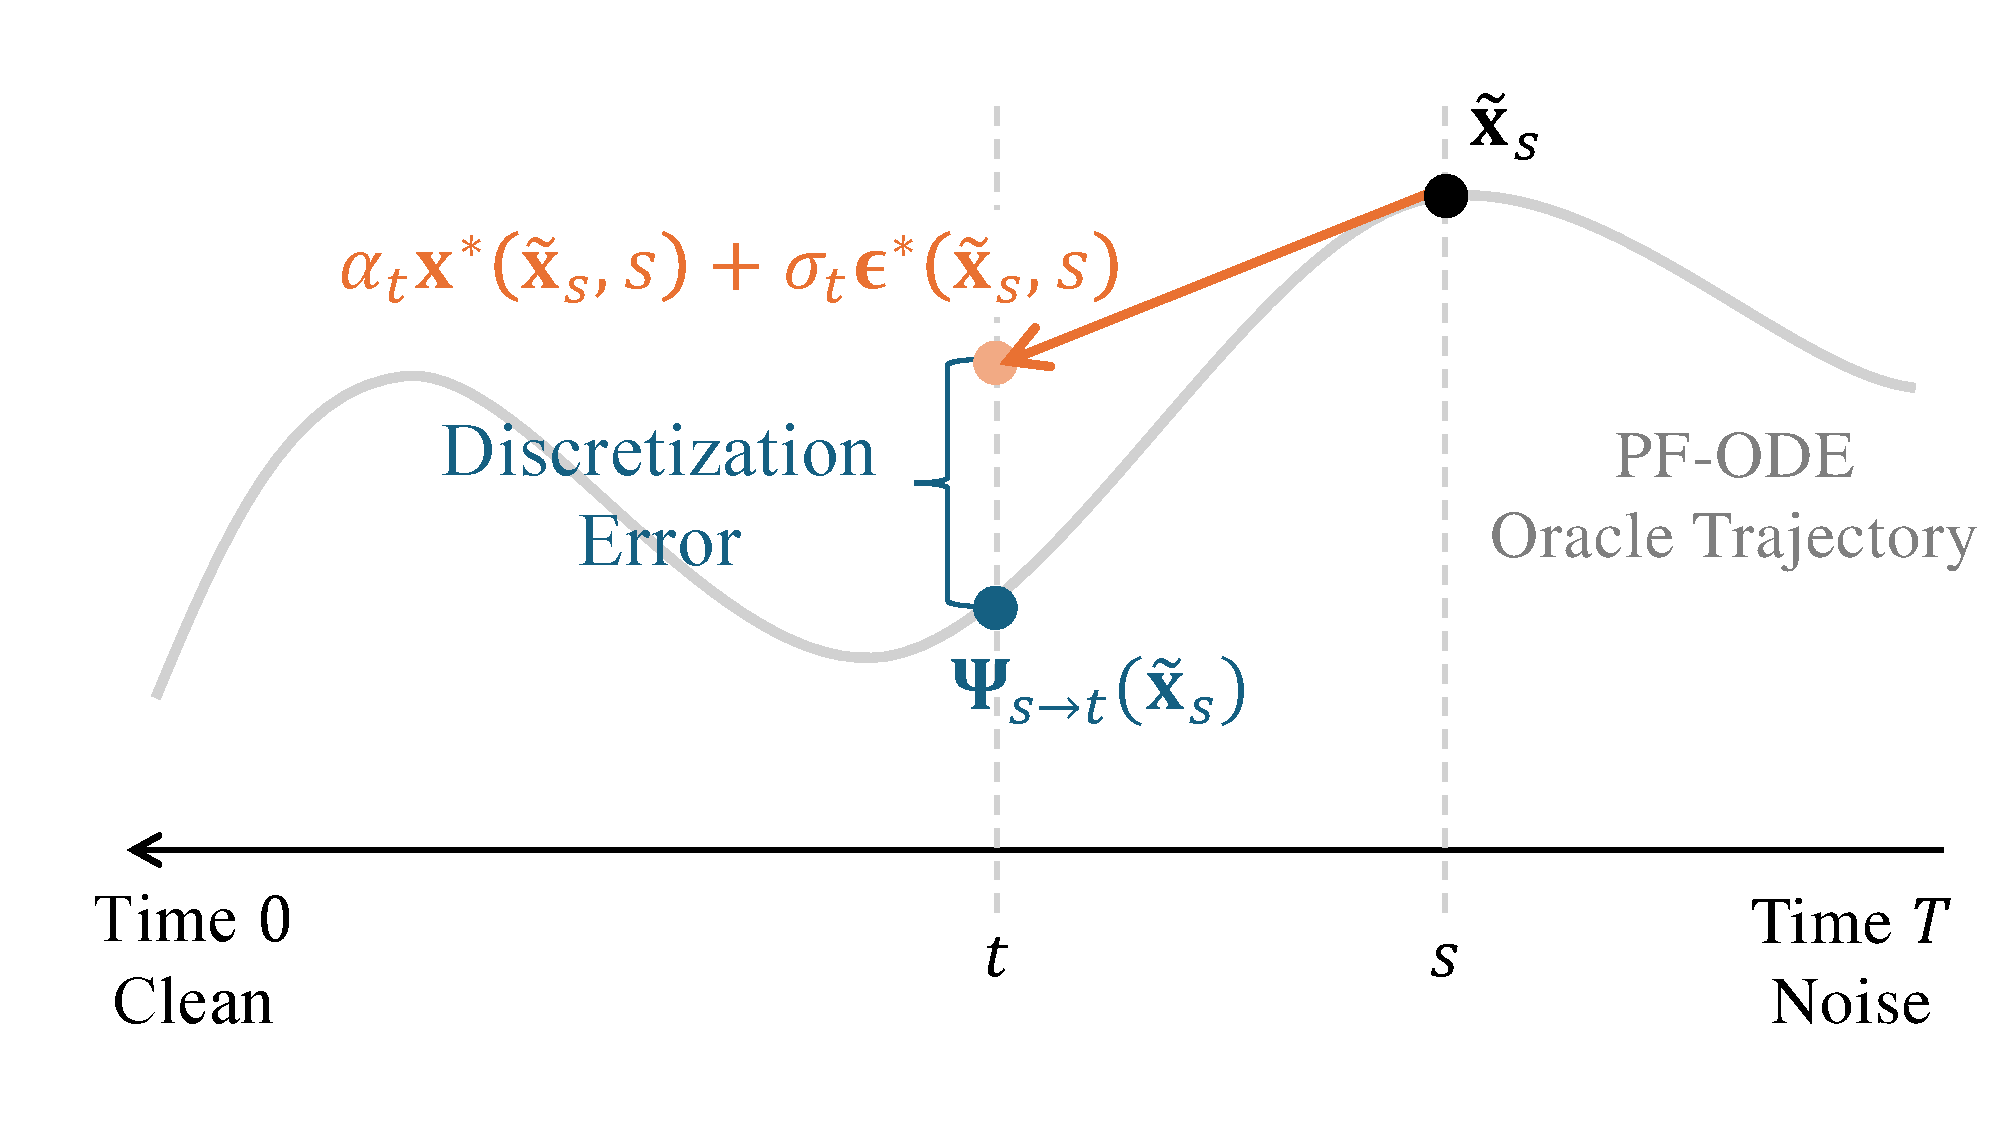
\includegraphics[width=0.86\linewidth]{Images/PartB/Euler.pdf}
    \caption{\textbfs{Finite-step DDIM versus the empirical PF-ODE flow.}
    Starting from $\tilde\rvx_s$, the empirical PF-ODE evolves continuously
    to $\widetilde\bPsi_{s\to t}(\tilde\rvx_s)$, whereas DDIM retains the
    start-time neural prediction over the whole interval while evolving the
    known schedule analytically. Their discrepancy is the one-step
    discretization error in \Cref{eq:ddim-local-defect}.
    \figcredit{Created by the authors.}}
    \label{fig:euler}
\end{figure}



\paragraph{Why Does the Prediction Held Fixed Matter?}
At any fixed state and time, the standard prediction parameterizations are
algebraically equivalent through \Cref{eq:predictions-equivalence}. A
finite-step solver, however, introduces an additional approximation by holding
one chosen prediction fixed over an interval. Such a freezing approximation is
preserved under a change of parameterization only when the converted prediction
also remains constant along the resulting approximate trajectory.

DDIM provides a particularly clean example. Let
\[
\widehat\rvx_0
:=
\rvx_{\bm{\phi}^\times}(\tilde\rvx_s,s),
\qquad
\widehat\beps
:=
\beps_{\bm{\phi}^\times}(\tilde\rvx_s,s),
\]
where, if only one quantity is directly predicted by the model, the other is
defined by the algebraic conversion in \Cref{eq:predictions-equivalence}.
Hence, by construction,
$\tilde\rvx_s=\alpha_s\widehat\rvx_0+\sigma_s\widehat\beps$.

Holding this start-time clean/noise pair fixed defines the DDIM interpolation
over the entire step:
\[
\tilde\rvx_\tau^{\mathrm{DDIM}}
=
\alpha_\tau\widehat\rvx_0
+
\sigma_\tau\widehat\beps,
\qquad
\tau\in[t,s].
\]
This requires no additional model evaluations: once
$(\widehat\rvx_0,\widehat\beps)$ is fixed at time $s$, the schedule
coefficients $(\alpha_\tau,\sigma_\tau)$ are known for every intermediate
$\tau$. At $\tau=s$ the expression recovers the starting state, while at
$\tau=t$ it gives the DDIM update. The intermediate values simply describe
the finite-step trajectory induced by the DDIM approximation.

The special role of noise and clean-data prediction is now immediate. Along
this trajectory,
\[
\frac{
\tilde\rvx_\tau^{\mathrm{DDIM}}
-
\sigma_\tau\widehat\beps
}{
\alpha_\tau
}
=
\widehat\rvx_0,
\qquad
\frac{
\tilde\rvx_\tau^{\mathrm{DDIM}}
-
\alpha_\tau\widehat\rvx_0
}{
\sigma_\tau
}
=
\widehat\beps.
\]
Thus, the algebraically converted clean and noise predictions remain constant
together along the DDIM trajectory. Consequently, holding
$\beps_{\bm{\phi}^\times}(\rvx_\tau,\tau)
\approx\beps_{\bm{\phi}^\times}(\tilde\rvx_s,s)$ or holding
$\rvx_{\bm{\phi}^\times}(\rvx_\tau,\tau)
\approx\rvx_{\bm{\phi}^\times}(\tilde\rvx_s,s)$ leads to the same DDIM
update. In this sense, $\widehat\rvx_0$ and $\widehat\beps$ are the two fixed
components of the DDIM shared-noise path, while
$(\alpha_\tau,\sigma_\tau)$ provide the known time-dependent weights.


However, score and velocity behave differently. DDIM keeps the inferred
clean/noise pair $(\widehat\rvx_0,\widehat\beps)$ fixed, but the score and
velocity obtained from this pair generally change with time.

For example, converting the fixed (at time $s$) noise estimate to score prediction at an
intermediate time $\tau$ gives
\[
\rvs(\tilde\rvx_\tau^{\mathrm{DDIM}},\tau)
=
-\frac{\widehat\beps}{\sigma_\tau}
=
\frac{\sigma_s}{\sigma_\tau}
\rvs_{\bm{\phi}^\times}(\tilde\rvx_s,s).
\]
Thus, even though $\widehat\beps$ is fixed, its corresponding score generally
varies with $\tau$ through the factor $1/\sigma_\tau$. Directly imposing
\[
\rvs_{\bm{\phi}^\times}(\rvx_\tau,\tau)
\approx
\rvs_{\bm{\phi}^\times}(\tilde\rvx_s,s),
\qquad
\tau\in[t,s],
\]
therefore makes a different finite-step approximation and generally yields a
different first-order factored solver. Similarly, the fixed clean/noise pair induces the velocity
\[
\frac{\diff}{\diff\tau}
\tilde\rvx_\tau^{\mathrm{DDIM}}
=
\alpha_\tau'\widehat\rvx_0
+
\sigma_\tau'\widehat\beps.
\]
This velocity generally changes with $\tau$ because the schedule derivatives
$\alpha_\tau'$ and $\sigma_\tau'$ change. Holding the raw velocity prediction
fixed instead,
$\rvv_{\bm{\phi}^\times}(\rvx_\tau,\tau)
\approx
\rvv_{\bm{\phi}^\times}(\tilde\rvx_s,s)$,
gives plain Euler in the original diffusion time; its relation to DDIM is
discussed in \Cref{subsec:ddim-classical-euler}.

\rmkb{
Prediction parameterizations are pointwise algebraically equivalent, but
finite-step freezing need not commute with a time-dependent conversion. DDIM
keeps a consistent start-time clean/noise pair fixed; the corresponding score
and complete velocity generally vary over the step. Hence directly freezing
the raw score or velocity defines a different first-order method. The velocity
case is quantified in \Cref{subsec:ddim-classical-euler}.
}



\subsection{Relation to Euler-Type Methods}
\label{subsec:ddim-classical-euler}


The discussion above shows that DDIM is a first-order method, but its relation
to the classical Euler method requires some care. Once the known diffusion
schedule is separated from the learned prediction, different first-order
schemes arise depending on \emph{what is held fixed over a finite step}.

We compare three one-evaluation constructions:
\begin{enumerate}
    \item \emph{plain Euler}, which holds the complete PF-ODE velocity fixed;
    \item \emph{exponential Euler}, which treats the known linear propagation
    analytically but holds the remaining coefficient-weighted residual fixed;
    \item \emph{DDIM}, which keeps the start-time clean/noise estimates fixed
    while retaining their finite-step evolution under the known diffusion
    schedule.
\end{enumerate}
These distinctions are easiest to see from two equivalent views of the same
DDIM update. The clean/noise form makes its difference from plain Euler
transparent, whereas the factored semilinear form clarifies its relation to
exponential Euler. We then identify the remaining discretization error and
show the precise sense in which DDIM itself can be viewed as an Euler method
after a schedule-aligned change of coordinates.


\paragraph{DDIM versus Plain Euler.}
DDIM and plain Euler use the same start-time model information, but propagate
it differently over a finite step. Plain Euler locally approximates the
complete PF-ODE velocity, whereas DDIM retains the finite-step evolution of
the known diffusion schedule while holding the model prediction fixed.
Consequently, for smooth schedules, the two updates agree to first order and
generally differ by terms of order $\mathcal O((\Delta s)^2)$. We make this
difference explicit below.

Consider one backward step from time $s$ to $t<s$, with
$\Delta s:=s-t>0$, and suppose the start-time clean and noise predictions are
algebraically consistent:
\[
\tilde\rvx_s
=
\alpha_s
\rvx_{\bm{\phi}^\times}(\tilde\rvx_s,s)
+
\sigma_s
\beps_{\bm{\phi}^\times}(\tilde\rvx_s,s).
\]
The corresponding empirical PF-ODE velocity at time $s$ is
\[
\rvv_{\bm{\phi}^\times}(\tilde\rvx_s,s)
=
\alpha_s'
\rvx_{\bm{\phi}^\times}(\tilde\rvx_s,s)
+
\sigma_s'
\beps_{\bm{\phi}^\times}(\tilde\rvx_s,s).
\]
Plain Euler holds this complete velocity fixed over the step, $\tau\in[t,s]$, and gives:
\[
\tilde\rvx_t^{\mathrm{Euler}}
=
\tilde\rvx_s
-
\Delta s\,
\rvv_{\bm{\phi}^\times}(\tilde\rvx_s,s).
\]
By contrast, DDIM keeps the clean/noise-prediction pair at the starting time fixed, while evolving the known schedule coefficients from $(\alpha_s,\sigma_s)$ to $(\alpha_t,\sigma_t)$:
\[
\tilde\rvx_t^{\mathrm{DDIM}}
=
\tilde\rvx_s
+
(\alpha_t-\alpha_s)
\rvx_{\bm{\phi}^\times}(\tilde\rvx_s,s)
+
(\sigma_t-\sigma_s)
\beps_{\bm{\phi}^\times}(\tilde\rvx_s,s).
\]
Their exact finite-step difference is therefore
\begin{align*}
\tilde\rvx_t^{\mathrm{DDIM}}
-
\tilde\rvx_t^{\mathrm{Euler}}
={}&
\left[
\alpha_t-\alpha_s+\Delta s\,\alpha_s'
\right]
\rvx_{\bm{\phi}^\times}(\tilde\rvx_s,s)
+
\left[
\sigma_t-\sigma_s+\Delta s\,\sigma_s'
\right]
\beps_{\bm{\phi}^\times}(\tilde\rvx_s,s).
\end{align*}
For smooth schedules,
\[
\alpha_t-\alpha_s+\Delta s\,\alpha_s'
=
\tfrac{(\Delta s)^2}{2}\alpha_s''
+
\mathcal O((\Delta s)^3), \quad
\sigma_t-\sigma_s+\Delta s\,\sigma_s'
=
\tfrac{(\Delta s)^2}{2}\sigma_s''
+
\mathcal O((\Delta s)^3).
\]
Hence,
\begin{align*}
\tilde\rvx_t^{\mathrm{DDIM}}
-
\tilde\rvx_t^{\mathrm{Euler}}
=
\tfrac{(\Delta s)^2}{2}
\left[
\alpha_s''
\rvx_{\bm{\phi}^\times}(\tilde\rvx_s,s)
+
\sigma_s''
\beps_{\bm{\phi}^\times}(\tilde\rvx_s,s)
\right]
+
\mathcal O((\Delta s)^3).
\end{align*}
Thus, DDIM and plain Euler agree to first order but generally differ over a
finite step. Plain Euler replaces the finite schedule changes
$(\alpha_t-\alpha_s,\sigma_t-\sigma_s)$ by their local linearizations,
whereas DDIM retains the finite schedule evolution analytically.

A useful special case follows immediately. If both $\alpha_\tau$ and
$\sigma_\tau$ are \emph{affine in $\tau$ over $[t,s]$}, then
\[
\alpha_t-\alpha_s=-\Delta s\,\alpha_s',
\qquad
\sigma_t-\sigma_s=-\Delta s\,\sigma_s',
\]
so DDIM and plain Euler coincide exactly. This includes, for example, the
schedules (see also discussion in \Cref{subsec:concept-why-v-affine}) 
\[(\alpha_t,\sigma_t)=(1,t)\quad \text{and}\quad (\alpha_t,\sigma_t)=(1-t,t) .
\]
Thus, the finite-step distinction between the
two methods is driven by the nonlinearity of the known schedule in the
original diffusion time.



\paragraph{DDIM versus Exponential Euler.}
The comparison above used the clean/noise representation to show how DDIM
differs from plain Euler in the original diffusion time. We now return to the
semilinear representation from the prologue to distinguish DDIM from
conventional exponential Euler. The difference is simple: both methods retain
the known linear evolution analytically, but they hold different quantities
fixed inside the remaining integral.

Under noise prediction, the factored PF-ODE in
\Cref{eq:general-semilinear-pfode} has
\[
a(\tau)=f(\tau),
\qquad
b(\tau)=\frac{g^2(\tau)}{2\sigma_\tau},
\qquad
\rmN_{\bm{\phi}^\times}
=
\beps_{\bm{\phi}^\times}.
\]
Its exact variation-of-constants formula contains the model-dependent term
\[
b(\tau)\beps_{\bm{\phi}^\times}(\rvx_\tau,\tau).
\]

Conventional exponential Euler treats this coefficient-weighted quantity as a
single residual and holds the whole residual fixed at the beginning of the
step:
\[
b(\tau)\beps_{\bm{\phi}^\times}(\rvx_\tau,\tau)
\approx
b(s)\beps_{\bm{\phi}^\times}(\tilde\rvx_s,s), \quad\tau\in[t,s]
\]
It therefore gives
\[
\tilde\rvx_t^{\mathrm{ExpEuler}}
=
\mathcal E(s\shortrightarrow t)\tilde\rvx_s
+
b(s)
\left[
\int_s^t
\mathcal E(\tau\shortrightarrow t)
\diff\tau
\right]
\beps_{\bm{\phi}^\times}(\tilde\rvx_s,s).
\]

DDIM uses the finer factorization emphasized in the prologue. Since
$b(\tau)$ is known from the diffusion schedule, it remains inside the
integral; only the neural prediction is held fixed:
\[
\beps_{\bm{\phi}^\times}(\rvx_\tau,\tau)
\approx
\beps_{\bm{\phi}^\times}(\tilde\rvx_s,s).
\]
Hence,
\[
\tilde\rvx_t^{\mathrm{DDIM}}
=
\mathcal E(s\shortrightarrow t)\tilde\rvx_s
+
\left[
\int_s^t
\mathcal E(\tau\shortrightarrow t)b(\tau)
\diff\tau
\right]
\beps_{\bm{\phi}^\times}(\tilde\rvx_s,s).
\]

The finite-step difference between the two updates therefore comes entirely
from the known coefficient $b(\tau)$:
\[
\tilde\rvx_t^{\mathrm{DDIM}}
-
\tilde\rvx_t^{\mathrm{ExpEuler}}
=
\left[
\int_s^t
\mathcal E(\tau\shortrightarrow t)
\bigl(b(\tau)-b(s)\bigr)
\diff\tau
\right]
\beps_{\bm{\phi}^\times}(\tilde\rvx_s,s).
\]
For smooth $b$,
\[
\tilde\rvx_t^{\mathrm{DDIM}}
-
\tilde\rvx_t^{\mathrm{ExpEuler}}
=
\frac{(\Delta s)^2}{2}
b'(s)
\beps_{\bm{\phi}^\times}(\tilde\rvx_s,s)
+
\mathcal O((\Delta s)^3).
\]
Thus, DDIM and conventional exponential Euler agree to first order. The only
difference is that exponential Euler freezes $b(\tau)$ at $b(s)$ together
with the neural prediction, while DDIM keeps the known variation of
$b(\tau)$. Therefore, the two updates coincide exactly whenever $b(\tau)$ is constant
over the step, including the constant-$b$ setting used in the Prologue
example.

Together with the preceding plain-Euler comparison, the three first-order
rules differ only in how much known structure is retained before making the
constant approximation on $\tau\in[t,s]$:
\[
\begin{array}{rcl}
\text{Plain Euler}
&:&
f(\tau)\rvx_\tau+b(\tau)\beps_\tau
\;\approx\;
f(s)\tilde\rvx_s+b(s)\widehat\beps,
\\[4pt]
\text{Exponential Euler}
&:&
b(\tau)\beps_\tau
\;\approx\;
b(s)\widehat\beps,
\\[4pt]
\text{DDIM}
&:&
\beps_\tau
\;\approx\;
\widehat\beps,
\end{array}
\]
where
$\widehat\beps
:=
\beps_{\bm{\phi}^\times}(\tilde\rvx_s,s)$.
All three use the same single neural-network evaluation at the beginning of
the step. Plain Euler approximates the complete velocity; exponential Euler
first retains the known linear propagation; DDIM additionally retains the
known coefficient $b(\tau)$ and approximates only the neural prediction.

This hierarchy concerns which analytically known terms are preserved, rather
than a universal ordering of one-step errors. Its main numerical consequence
is that the remaining approximation in DDIM can be isolated entirely to the
variation of the neural prediction, as we show next.



\paragraph{What Error Does Each Method Still Make?}
The comparisons above describe how the three numerical updates differ from one
another. We now compare each update with the exact empirical PF-ODE flow.
For this local-error analysis, suppose the step starts from an exact empirical
state $\rvx_s$ at time $s$.

For plain Euler, the exact empirical flow can be written in the direct velocity
form as
\[
\widetilde\bPsi_{s\to t}(\rvx_s)
=
\rvx_s
+
\int_s^t
\rvv_{\bm{\phi}^\times}(\rvx_\tau,\tau)
\diff\tau.
\]
Since plain Euler holds the complete velocity fixed at its start-time value,
its exact one-step defect is
\begin{align*}
\widetilde\bPsi_{s\to t}(\rvx_s)
-
\tilde\rvx_t^{\mathrm{Euler}}
=
\int_s^t
\Big[
\rvv_{\bm{\phi}^\times}(\rvx_\tau,\tau)
-
\rvv_{\bm{\phi}^\times}(\rvx_s,s)
\Big]
\diff\tau.
\end{align*}

For exponential Euler, the known linear propagation is already treated
analytically, but the coefficient-weighted residual
$b(\tau)\beps_{\bm{\phi}^\times}(\rvx_\tau,\tau)$ is held fixed. Hence
\begin{align*}
\widetilde\bPsi_{s\to t}(\rvx_s)
-
\tilde\rvx_t^{\mathrm{ExpEuler}}
=
\int_s^t
\mathcal E(\tau\shortrightarrow t)
\Big[
b(\tau)
\beps_{\bm{\phi}^\times}(\rvx_\tau,\tau)
-
b(s)
\beps_{\bm{\phi}^\times}(\rvx_s,s)
\Big]
\diff\tau.
\end{align*}

Finally, DDIM retains both the known linear propagation and the known
coefficient $b(\tau)$, and holds only the neural prediction fixed:
\begin{align}
\label{eq:ddim-local-defect}
\widetilde\bPsi_{s\to t}(\rvx_s)
-
\tilde\rvx_t^{\mathrm{DDIM}}
=
\int_s^t
\mathcal E(\tau\shortrightarrow t)b(\tau)
\Big[
\beps_{\bm{\phi}^\times}(\rvx_\tau,\tau)
-
\beps_{\bm{\phi}^\times}(\rvx_s,s)
\Big]
\diff\tau.
\end{align}

These identities reveal the relevant notion of smoothness for each first-order
scheme. If the corresponding quantity varies slowly along the exact empirical
trajectory, then the one-step approximation is accurate. More precisely,
with $\Delta s:=s-t$, standard smoothness gives
\begin{align*}
\left\|
\widetilde\bPsi_{s\to t}(\rvx_s)
-
\tilde\rvx_t^{\mathrm{Euler}}
\right\|
&\le
\frac{(\Delta s)^2}{2}
\sup_{\tau\in[t,s]}
\left\|
\tfrac{\diff}{\diff\tau}
\rvv_{\bm{\phi}^\times}(\rvx_\tau,\tau)
\right\|,
\\
\left\|
\widetilde\bPsi_{s\to t}(\rvx_s)
-
\tilde\rvx_t^{\mathrm{ExpEuler}}
\right\|
&\le
\frac{(\Delta s)^2}{2}
\sup_{\tau\in[t,s]}
\left|
\mathcal E(\tau\shortrightarrow t)
\right|\cdot
\sup_{\tau\in[t,s]}
\left\|
\tfrac{\diff}{\diff\tau}
\left[
b(\tau)
\beps_{\bm{\phi}^\times}(\rvx_\tau,\tau)
\right]
\right\|,
\\
\left\|
\widetilde\bPsi_{s\to t}(\rvx_s)
-
\tilde\rvx_t^{\mathrm{DDIM}}
\right\|
&\le
\frac{(\Delta s)^2}{2}
\sup_{\tau\in[t,s]}
\left|
\mathcal E(\tau\shortrightarrow t)b(\tau)
\right| \cdot
\sup_{\tau\in[t,s]}
\left\|
\tfrac{\diff}{\diff\tau}
\beps_{\bm{\phi}^\times}(\rvx_\tau,\tau)
\right\|.
\end{align*}

Under the usual smoothness and stability assumptions, all three methods are
\emph{globally first order} and require only one neural-network evaluation per
step. Moreover, each method is exact on a step when the quantity it holds
fixed is in fact constant along the exact empirical trajectory: the complete
PF-ODE velocity for plain Euler, the coefficient-weighted residual
$b(\tau)\beps_{\bm{\phi}^\times}(\rvx_\tau,\tau)$ for exponential Euler, and
the noise prediction
$\beps_{\bm{\phi}^\times}(\rvx_\tau,\tau)$ for DDIM.

Accordingly, there is no universal error ordering among the three methods:
each is most accurate when the quantity it holds fixed varies slowly over the
step. DDIM is particularly well suited to regimes where the neural prediction
changes slowly but the known diffusion schedule changes appreciably, since it
retains the latter analytically. Exploiting more known structure can therefore
reduce discretization error, but does not guarantee a smaller error on every
individual step.


The errors discussed here are numerical discretization errors relative to the
empirical PF-ODE; model mismatch between the empirical and oracle PF-ODEs is
a separate source of error.


\paragraph{A Precise Euler Interpretation of DDIM.}
Although DDIM and plain Euler agree to first order, they generally give
different finite-step updates in the original state $\rvx$ and diffusion time
$t$. There is, however, an exact Euler interpretation after a
schedule-aligned change of both the state and the time coordinate.

Under noise prediction, define
\begin{equation*}
\rvy_t
:=
\frac{\rvx_t}{\alpha_t},
\qquad
\rho_t
:=
\frac{\sigma_t}{\alpha_t}.
\end{equation*}
The two transformations play complementary roles. The state normalization
$\rvx_t\mapsto\rvx_t/\alpha_t$ factors out the known signal scaling
$\alpha_t$, while the new clock
$\rho_t=\sigma_t/\alpha_t$ measures progress by the noise-to-signal ratio
rather than by the original diffusion time.

To see this first at the conditional level, consider a fixed pair
$(\rvx_0,\beps)$ in the Gaussian perturbation path
\[
\rvx_t
=
\alpha_t\rvx_0+\sigma_t\beps,
\qquad
\beps\sim\mathcal N(\mathbf 0,\mathbf I).
\]
Here, $\beps$ is a fixed latent noise realization, not a neural prediction.
The transformed state satisfies
\[
\rvy_t
=
\frac{\rvx_t}{\alpha_t}
=
\rvx_0+\rho_t\beps.
\]
Hence, along this particular conditional path,
\[
\frac{\diff\rvy}{\diff\rho}
=
\beps.
\]
Thus, for fixed $(\rvx_0,\beps)$, the known schedule dependence becomes affine
in the transformed coordinate $\rho$.

The corresponding empirical PF-ODE has the same coordinate structure, but
the fixed latent noise $\beps$ is replaced by the learned, state-dependent
noise prediction. Using \Cref{eq:noise_pf_ode},
\[
\frac{\diff\rvx_t}{\diff t}
=
\frac{\alpha_t'}{\alpha_t}\rvx_t
+
\left(
\sigma_t'
-
\frac{\alpha_t'}{\alpha_t}\sigma_t
\right)
\beps_{\bm{\phi}^\times}(\rvx_t,t),
\]
we obtain
\begin{align}
\frac{\diff\rvy_t}{\diff t}
=
\frac{1}{\alpha_t}
\left(
\frac{\diff\rvx_t}{\diff t}
-
\frac{\alpha_t'}{\alpha_t}\rvx_t
\right)=
\frac{\diff\rho_t}{\diff t}\,
\beps_{\bm{\phi}^\times}(\rvx_t,t).
\label{eq:ddim-coordinate-ode-t}
\end{align}
Hence, on any interval where $\alpha_t>0$ and $\rho_t$ is strictly monotone,
we may use $\rho$ as the time coordinate. Writing $t=t(\rho)$ and defining
the transformed neural field
\[
\bar{\beps}_{\bm{\phi}^\times}(\rvy,\rho)
:=
\beps_{\bm{\phi}^\times}
\bigl(
\alpha_{t(\rho)}\rvy,
t(\rho)
\bigr),
\]
the empirical PF-ODE becomes
\begin{equation}
\label{eq:ddim-coordinate-ode-rho}
\frac{\diff\rvy}{\diff\rho}
=
\bar{\beps}_{\bm{\phi}^\times}(\rvy,\rho).
\end{equation}
The spatial and temporal dependence of the model therefore remains present;
it is simply expressed in the transformed variables $(\rvy,\rho)$.

Explicit Euler applied to \Cref{eq:ddim-coordinate-ode-rho} from
$\rho_s$ to $\rho_t$ gives
\[
\tilde\rvy_t
=
\tilde\rvy_s
+
(\rho_t-\rho_s)
\bar{\beps}_{\bm{\phi}^\times}(\tilde\rvy_s,\rho_s).
\]
Since
\[
\bar{\beps}_{\bm{\phi}^\times}(\tilde\rvy_s,\rho_s)
=
\beps_{\bm{\phi}^\times}(\tilde\rvx_s,s),
\]
substituting
$\rvy=\rvx/\alpha$ and $\rho=\sigma/\alpha$ yields
\[
\tilde\rvx_t
=
\frac{\alpha_t}{\alpha_s}\tilde\rvx_s
+
\alpha_t
\left(
\frac{\sigma_t}{\alpha_t}
-
\frac{\sigma_s}{\alpha_s}
\right)
\beps_{\bm{\phi}^\times}(\tilde\rvx_s,s),
\]
which is exactly the deterministic DDIM update.

\msgu{Coordinate Choice Is Part of the Numerical Method}{}{
An invertible change of state and time coordinates gives an equivalent
representation of the same continuous ODE solution. A finite-step
discretization, however, is generally not invariant to that representation:
``change coordinates and then apply Euler'' need not equal
``apply Euler and then change coordinates''.


The numerical significance is that a suitable coordinate system can absorb
analytically known parts of the dynamics before discretization. In DDIM,
$\rvx/\alpha$ removes the known signal scaling and
$\rho=\sigma/\alpha$ absorbs the corresponding schedule-dependent time
scaling, leaving the transformed neural field
$\bar{\beps}_{\bm{\phi}^\times}(\rvy,\rho)$ as the quantity approximated by
Euler. Thus DDIM generally differs from plain Euler in $(\rvx,t)$, while it is
exactly explicit Euler in the schedule-aligned coordinates
$(\rvy,\rho)$.
}

A dual construction holds under clean-data prediction. Normalizing the state by $\sigma_t$ and using $\alpha_t/\sigma_t$ as the time coordinate gives 
\[
\frac{\diff}{\diff t} \left( \frac{\rvx_t}{\sigma_t} \right) = \frac{\diff}{\diff t} \left( \frac{\alpha_t}{\sigma_t} \right) \rvx_{\bm{\phi}^\times}(\rvx_t,t), 
\] 
so the clean-data form of DDIM is likewise explicit Euler in its corresponding schedule-aligned coordinates.

This \emph{state--time change-of-coordinates viewpoint} also previews the role
of coordinate choice in higher-order diffusion solvers. DPM-Solver, developed
later in \Cref{sec:dpm}, uses the half-log SNR
\[
\lambda_t
:=
\log\frac{\alpha_t}{\sigma_t},
\]
which is directly related to DDIM's Euler clock:
\[
\rho_t
=
\frac{\sigma_t}{\alpha_t}
=
e^{-\lambda_t},
\qquad
\diff\rho
=
-e^{-\lambda}\diff\lambda.
\]
Therefore, the exact transformed equation
\[
\frac{\diff\rvy}{\diff\rho}
=
\bar{\beps}_{\bm{\phi}^\times}(\rvy,\rho)
\]
can equivalently be integrated as
\[
\rvy_t
=
\rvy_s
-
\int_{\lambda_s}^{\lambda_t}
e^{-\lambda}
\hat{\beps}_{\bm{\phi}^\times}
(\hat\rvx_\lambda,\lambda)
\diff\lambda,
\]
with the usual $\lambda$-parameterized model notation introduced later in
\Cref{sec:dpm}.

At first order, holding the neural prediction fixed while retaining the known
change-of-variable weight gives the same finite-step update, so
DPM-Solver-1 is exactly DDIM. Beyond first order, however, the coordinate in
which the state--time-dependent neural prediction is approximated becomes part
of the numerical method. DPM-Solver uses $\lambda$ because it yields an
exponentially weighted integral with convenient higher-order expansions.



\subsection{(Optional) The Original Variational Perspective on DDIM}\label{subsec:ddim}

The PF-ODE perspective above explains deterministic DDIM as a numerical
solver. Historically, however, DDIM was introduced from the variational
viewpoint of DDPM. Its starting question is different:
\emph{does the denoising objective uniquely determine how noisy states at
different times must be coupled?}

\paragraph{Revisiting DDPM's Variational View.}
Recall that DDPM introduces a fixed Markovian inference process whose
one-time perturbation marginals take the Gaussian form
\[
p_t(\rvx_t|\rvx_0)
=
\mathcal N
\bigl(
\rvx_t;
\alpha_t\rvx_0,
\sigma_t^2\rmI
\bigr).
\]
The corresponding variational derivation involves tractable conditionals
such as
$p(\rvx_t|\rvx_s,\rvx_0)$ for $t<s$, while the learned reverse model used
for generation cannot condition directly on the unknown clean sample
$\rvx_0$ and instead relies on the diffusion-model prediction.

The key observation behind DDIM concerns the denoising objective. We recall that a noise-prediction DDPM loss can be written as
\[
\E_t
\E_{\rvx_0,\beps}
\left[
\left\|
\beps_{\bm{\phi}}
\bigl(
\alpha_t\rvx_0+\sigma_t\beps,t
\bigr)
-
\beps
\right\|_2^2
\right],
\]
which depends on the inference process through the one-time marginals
$p_t(\rvx_t|\rvx_0)$, rather than through the full joint coupling of
$\rvx_1,\ldots,\rvx_T$ conditioned on $\rvx_0$.


\paragraph{Original DDIM Motivation.}
The central observation behind DDIM is that the denoising training objective
does not uniquely determine how noisy states at different times are coupled.
For a fixed clean sample $\rvx_0$, the usual denoising surrogate is determined
by the one-time perturbation marginals
$p_t(\rvx_t|\rvx_0)$, whereas many different joint processes across time can
share exactly the same marginals. DDIM exploits this freedom: it preserves
the perturbation marginals used during training, while changing the coupling
between different noise levels.

Concretely, for any $t<s$, consider a conditional transition
${\color{orange}\pi(\rvx_t|\rvx_s,\rvx_0)}$. We require it to be
\emph{one-step marginally consistent}:
\begin{mdframed}
\begin{align}
\label{eq:ddim-reverse-kernel-def}
\int
{\color{orange}\pi(\rvx_t|\rvx_s,\rvx_0)}
\,p_s(\rvx_s|\rvx_0)
\diff\rvx_s
=
p_t(\rvx_t|\rvx_0).
\end{align}
\end{mdframed}
In words, if
$\rvx_s\sim p_s(\cdot|\rvx_0)$, then applying the chosen transition once
produces
$\rvx_t\sim p_t(\cdot|\rvx_0)$. Hence, the marginal distribution at each
noise level is preserved even though the dependence between
$\rvx_s$ and $\rvx_t$ may be changed.

The Bayesian reverse posterior induced by the original Markovian DDPM
forward process is one valid choice of such a transition,\footnote{For the
Markov forward process,
$\rvx_0\to\rvx_t\to\rvx_s$ with $t<s$, the conditional posterior
$p(\rvx_t|\rvx_s,\rvx_0)$ satisfies
\[
p_t(\rvx_t|\rvx_0)
=
\int
p(\rvx_t|\rvx_s,\rvx_0)
\,p_s(\rvx_s|\rvx_0)
\diff\rvx_s
\]
by the law of total probability.}
but it is not uniquely determined by the marginals. DDIM instead allows
other marginal-consistent couplings, including transitions directly between
widely separated noise levels. This is the probabilistic reason that the
same trained denoiser can be reused on a coarser sampling grid with skipped
intermediate times.

\paragraph{Derivation of Discrete-Time DDIM.}
We now make the coupling freedom above explicit for the Gaussian perturbation
model
\[
p_t(\rvx_t|\rvx_0)
:=
\mathcal{N}
\bigl(
\rvx_t;
\alpha_t\rvx_0,
\sigma_t^2\mathbf{I}
\bigr),
\qquad
\rvx_0\sim p_{\mathrm{data}}.
\]
The goal is to construct, for any $t<s$, a conditional transition
${\color{orange}\pi(\rvx_t|\rvx_s,\rvx_0)}$ that satisfies the
marginal-consistency condition in \Cref{eq:ddim-reverse-kernel-def}, without
requiring it to coincide with the Bayesian posterior associated with the
original Markov forward process.

A natural choice is the Gaussian family
\begin{align}
\label{eq:ddim-reverse-kernel-param}
{\color{orange}\pi(\rvx_t|\rvx_s,\rvx_0)}
=
\mathcal{N}
\bigl(
\rvx_t;\,
a_{t,s}\rvx_0+b_{t,s}\rvx_s,\,
c_{t,s}^2\mathbf{I}
\bigr),
\end{align}
where $(a_{t,s},b_{t,s},c_{t,s})$ determine how the state at time $s$,
the clean sample, and newly injected noise are combined.

To impose marginal consistency, first draw
\[
\rvx_s
=
\alpha_s\rvx_0+\sigma_s\beps',
\qquad
\beps'\sim\mathcal{N}(\mathbf{0},\mathbf{I}),
\]
and then draw $\rvx_t$ from
\Cref{eq:ddim-reverse-kernel-param}. Equivalently,
\begin{align}
\label{eq:ddim-derivation}
\begin{aligned}
\rvx_t
&=
a_{t,s}\rvx_0
+
b_{t,s}\rvx_s
+
c_{t,s}\beps
\\
&=
a_{t,s}\rvx_0
+
b_{t,s}
\bigl(
\alpha_s\rvx_0+\sigma_s\beps'
\bigr)
+
c_{t,s}\beps
\\
&=
\bigl(
a_{t,s}+b_{t,s}\alpha_s
\bigr)\rvx_0
+
\sqrt{
b_{t,s}^2\sigma_s^2+c_{t,s}^2
}\,
\beps'',
\end{aligned}
\end{align}
where $\beps$ and $\beps'$ are independent standard Gaussian variables, and
$\beps''$ is a standard Gaussian representing their normalized linear
combination.

For the resulting marginal to equal the prescribed perturbation marginal $\rvx_t
\sim
p_t(\rvx_t|\rvx_0)
=
\mathcal{N}
\bigl(
\rvx_t;
\alpha_t\rvx_0,
\sigma_t^2\mathbf{I}
\bigr)$, the means and variances must agree. Therefore,
\begin{align*}
\alpha_t
&=
a_{t,s}+b_{t,s}\alpha_s,
\\
\sigma_t^2
&=
b_{t,s}^2\sigma_s^2+c_{t,s}^2.
\end{align*}

The important point is that these are only two constraints on the three
coefficients $(a_{t,s},b_{t,s},c_{t,s})$. Hence, the prescribed marginals do
\emph{not} determine a unique transition between $s$ and $t$. We may choose
$c_{t,s}$ as a free parameter, with
$0\leq c_{t,s}\leq\sigma_t$, and solve for the remaining coefficients.
Choosing the nonnegative branch gives
\begin{align}
\label{eq:ddim-coefficients}
b_{t,s}
&=
\frac{
\sqrt{\sigma_t^2-c_{t,s}^2}
}{
\sigma_s
},
\qquad
a_{t,s}
=
\alpha_t-\alpha_s b_{t,s}.
\end{align}
The nonnegative choice of $b_{t,s}$ gives the standard DDIM coupling.

Substituting \Cref{eq:ddim-coefficients} into
\Cref{eq:ddim-reverse-kernel-param} yields
\begin{align}
\label{eq:ddim-reverse-kernel-result}
{\color{orange}\pi(\rvx_t|\rvx_s,\rvx_0)}
=
\mathcal{N}
\left(
\rvx_t;\,
\alpha_t\rvx_0
+
\frac{
\sqrt{\sigma_t^2-c_{t,s}^2}
}{
\sigma_s
}
\bigl(
\rvx_s-\alpha_s\rvx_0
\bigr),
\,
c_{t,s}^2\mathbf{I}
\right).
\end{align}

This expression makes the coupling freedom explicit. The term
$\rvx_s-\alpha_s\rvx_0$ is the noise component already present in
$\rvx_s$, while $c_{t,s}$ controls how much \emph{new} Gaussian noise is
introduced in the transition from $s$ to $t$. Varying $c_{t,s}$ therefore
changes the coupling between the two noise levels while preserving the same
target marginal $p_t(\rvx_t|\rvx_0)$.

\rmkb{
The chosen transition
${\color{orange}\pi(\rvx_t|\rvx_s,\rvx_0)}$
is generally different from the Bayesian posterior associated with the
original Markov forward process. That posterior is recovered by one
particular choice of $c_{t,s}$, discussed below. Other choices define
different marginal-consistent couplings, including the deterministic DDIM
coupling obtained when $c_{t,s}=0$.
}


\paragraph{DDIM Sampler (Step $s\to t$).}
The marginal-consistent kernel
${\color{orange}\pi(\rvx_t|\rvx_s,\rvx_0)}$ in
\Cref{eq:ddim-reverse-kernel-result} still conditions on the unknown clean
sample $\rvx_0$. During generation, DDIM replaces $\rvx_0$ by the clean-data
estimate obtained from the pre-trained diffusion model. Under
$\beps$-prediction, we define
\[
\rvx_{\bm{\phi}^\times}(\rvx_s,s)
:=
\frac{
\rvx_s
-
\sigma_s\beps_{\bm{\phi}^\times}(\rvx_s,s)
}{
\alpha_s
},
\]
and use the plug-in transition
\[
p_{\bm{\phi}^\times}(\rvx_t|\rvx_s)
:=
{\color{orange}\pi
\bigl(
\rvx_t
\,\big|\,
\rvx_s,
\rvx_{\bm{\phi}^\times}(\rvx_s,s)
\bigr)}.
\]
Substituting this estimate into
\Cref{eq:ddim-reverse-kernel-result} yields
\begin{mdframed}
\[
\rvx_t
=
\frac{\alpha_t}{\alpha_s}\rvx_s
+
\left(
\sqrt{\sigma_t^2-c_{t,s}^2}
-
\frac{\alpha_t}{\alpha_s}\sigma_s
\right)
\beps_{\bm{\phi}^\times}(\rvx_s,s)
+
c_{t,s}\beps_t,
\qquad
\beps_t\sim\mathcal{N}(\mathbf{0},\mathbf{I}).
\]
\end{mdframed}
Thus, the model prediction determines the estimated clean/noise content
carried from $s$ to $t$, while the free coefficient
$c_{t,s}\in[0,\sigma_t]$ controls how much \emph{new} Gaussian noise is
injected during the step.

To interpret this degree of freedom, it is useful to compare with the
original Markov forward process. For $t<s$, define
\[
\alpha_{s|t}
:=
\frac{\alpha_s}{\alpha_t},
\qquad
\sigma_{s|t}^2
:=
\sigma_s^2-\alpha_{s|t}^2\sigma_t^2,
\]
so that
\[
p(\rvx_s|\rvx_t)
=
\mathcal{N}
\bigl(
\rvx_s;
\alpha_{s|t}\rvx_t,
\sigma_{s|t}^2\mathbf I
\bigr).
\]
Gaussian conditioning gives the corresponding posterior variance
\[
\operatorname{Var}
\bigl(
\rvx_t|\rvx_s,\rvx_0
\bigr)
=
\frac{\sigma_t^2}{\sigma_s^2}
\sigma_{s|t}^2\mathbf I.
\]
This identifies the DDPM posterior as one particular member of the
marginal-consistent family above and makes the role of $c_{t,s}$ explicit:

\begin{itemize}
\item \textbfs{DDPM Step (Posterior Variance).}
Choosing
\[
c_{t,s}
=
\frac{\sigma_t}{\sigma_s}\sigma_{s|t}
\]
matches the posterior variance of the original Markov forward process.
Together with the nonnegative branch in
\Cref{eq:ddim-coefficients}, the conditional kernel
${\color{orange}\pi(\rvx_t|\rvx_s,\rvx_0)}$ then coincides with the
Bayesian posterior $p(\rvx_t|\rvx_s,\rvx_0)$ of that process.

\item \textbfs{Deterministic DDIM ($\eta=0$).}
At the opposite extreme, setting $c_{t,s}=0$ removes all newly injected
noise. The practical update becomes
\[
\rvx_t
=
\frac{\alpha_t}{\alpha_s}\rvx_s
+
\left(
\sigma_t
-
\frac{\alpha_t}{\alpha_s}\sigma_s
\right)
\beps_{\bm{\phi}^\times}(\rvx_s,s),
\]
which is exactly the deterministic DDIM update derived earlier from the
PF-ODE.

At the conditional level, its shared-noise interpretation is especially
simple: if
$\rvx_s=\alpha_s\rvx_0+\sigma_s\beps$, then the deterministic transition
gives
\[
\rvx_t
=
\alpha_t\rvx_0+\sigma_t\beps.
\]
Thus, no new noise is introduced; the same pair $(\rvx_0,\beps)$ is carried
across the step while only the known schedule coefficients change.

\item \textbfs{Interpolation.}
More generally, define
\begin{align}
\label{eq:eta-ddim}
c_{t,s}
=
\eta\,
\frac{\sigma_t}{\sigma_s}\,
\sigma_{s|t},
\qquad
\eta\in[0,1].
\end{align}
The parameter $\eta$ continuously controls the stochasticity of the
transition: $\eta=0$ gives deterministic DDIM, whereas $\eta=1$ matches the
posterior variance of the corresponding DDPM Markov transition.
\end{itemize}

Hence, the DDIM family separates two ingredients that are fixed differently:
the perturbation marginals are kept unchanged, while the coupling between
successive noise levels can be varied through $c_{t,s}$. Deterministic DDIM
corresponds to preserving the existing shared noise across the step, whereas
the DDPM posterior choice injects the amount of additional randomness
prescribed by the original Markov forward process.

\paragraph{Connection to Conditional Flow Matching.}
The deterministic DDIM construction above also provides a simple connection
to conditional flow matching (CFM) in \Cref{sec:flow-matching-framework}. The key is to distinguish two objects
associated with the same conditional Gaussian path: its \emph{finite-time
map} and its \emph{instantaneous velocity}. DDIM is related to the former,
whereas CFM is built from the latter.

Condition on a clean sample $\rvx_0$ and consider the shared-noise path
\[
\rvx_\tau
=
\alpha_\tau\rvx_0
+
\sigma_\tau\beps.
\]
For fixed $(\rvx_0,\beps)$, this is an exact conditional trajectory through
the Gaussian perturbation marginals
$p_\tau(\rvx_\tau|\rvx_0)$.

\textbfs{Finite-Time View: the Conditional DDIM Map.}
Suppose the trajectory is at $\rvx_s$ at time $s$. Since the same
$\beps$ is retained, eliminating it from
$\rvx_s=\alpha_s\rvx_0+\sigma_s\beps$ gives the exact conditional map
\[
\bPsi_{s\to t}(\rvx_s|\rvx_0)
=
\frac{\sigma_t}{\sigma_s}\rvx_s
+
\left(
\alpha_t
-
\alpha_s\frac{\sigma_t}{\sigma_s}
\right)\rvx_0.
\]
This map is exact \emph{conditioned on $\rvx_0$}. It is not yet the practical
DDIM sampler, because $\rvx_0$ is unknown during generation. Replacing
$\rvx_0$ by its start-time model prediction gives precisely the deterministic
DDIM update derived above.

\textbfs{Infinitesimal-Time View: the CFM Conditional Velocity.}
Instead of asking where the conditional path moves over a finite interval,
we may ask for its instantaneous direction. Differentiating
$\rvx_t=\alpha_t\rvx_0+\sigma_t\beps$ gives
\[
\frac{\diff\rvx_t}{\diff t}
=
\alpha_t'\rvx_0+\sigma_t'\beps.
\]
Using
\[
\beps
=
\frac{\rvx-\alpha_t\rvx_0}{\sigma_t},
\]
the same velocity can be written as a function of the current state:
\[
\rvv_t^*(\rvx|\rvx_0)
=
\frac{\sigma_t'}{\sigma_t}\rvx
+
\left(
\alpha_t'
-
\alpha_t\frac{\sigma_t'}{\sigma_t}
\right)\rvx_0.
\]
This is the conditional velocity associated with the Gaussian probability
path in conditional flow matching.

CFM then connects this conditional velocity to the marginal dynamics by
averaging over the posterior uncertainty about $\rvx_0$ at the current
state:
\begin{align*}
\rvv^*(\rvx,t)
&:=
\E_{\rvx_0\sim p(\rvx_0|\rvx_t=\rvx)}
\left[
\rvv_t^*(\rvx|\rvx_0)
\right]
\\
&=
\frac{\sigma_t'}{\sigma_t}\rvx
+
\left(
\alpha_t'
-
\alpha_t\frac{\sigma_t'}{\sigma_t}
\right)
\rvx^*(\rvx,t)
\\
&=
\alpha_t'\rvx^*(\rvx,t)
+
\sigma_t'\beps^*(\rvx,t),
\end{align*}
where we used
\[
\rvx^*(\rvx,t)
=
\E[\rvx_0|\rvx_t=\rvx],
\qquad
\rvx
=
\alpha_t\rvx^*(\rvx,t)
+
\sigma_t\beps^*(\rvx,t).
\]
The resulting $\rvv^*(\rvx,t)$ is exactly the oracle marginal PF-ODE
velocity.

\msgu{DDIM and CFM}{}{
The same conditional Gaussian path gives two views:
DDIM uses its finite-time map after replacing the unknown $\rvx_0$ by a
model prediction, while CFM uses its instantaneous conditional velocity.
Posterior averaging the latter gives the marginal PF-ODE velocity.
}

This connection is exact at the level of the conditional path and its
instantaneous velocity. It does \emph{not} imply that a finite DDIM step is
the exact marginal PF-ODE flow: DDIM keeps the prediction inferred at the
beginning of the step fixed, whereas the exact marginal PF-ODE velocity
changes continuously with the evolving state.


\clearpage
\newpage

\section{\texorpdfstring{DEIS}{DEIS}}\label{sec:exponential}

In the factored exponential-integrator formula
(\Cref{eq:variation_of_constants}),
\[
\int_s^t
\frac{g^2(\tau)}{2\sigma_\tau}\,
\mathcal E(\tau\shortrightarrow t)\,
\beps_{\bm{\phi}^\times}(\rvx_\tau,\tau)
\diff\tau,
\]
all schedule-dependent factors are known; the only unknown quantity along the
trajectory is the neural prediction
$\beps_{\bm{\phi}^\times}(\rvx_\tau,\tau)$. DDIM makes the simplest
first-order approximation by holding this prediction fixed at the beginning of
the step,
\[
\beps_{\bm{\phi}^\times}(\rvx_\tau,\tau)
\approx
\beps_{\bm{\phi}^\times}(\rvx_s,s),
\qquad
\tau\in[t,s].
\]
This approximation can become inaccurate over larger steps when the neural
prediction varies appreciably along the trajectory.

DEIS~\citep{zhang2022fast} improves on this idea without introducing
additional model evaluations within the current step. Inspired by classical
multistep methods such as Adams--Bashforth
(see \Cref{app:de-solver-examples}), it reuses model predictions from previous
completed steps as \emph{anchors} and fits a polynomial that extrapolates
their recent variation into the next step. The polynomial then replaces the
unknown neural prediction inside the integral, while the known
schedule-dependent weight
$\tfrac{g^2(\tau)}{2\sigma_\tau}
\mathcal E(\tau\shortrightarrow t)$
is retained analytically. Thus, DEIS extends the constant approximation of
DDIM to a higher-order multistep polynomial approximation.

From the classical numerical viewpoint, DEIS is therefore an
Adams--Bashforth-type multistep method within the factored
exponential-integrator framework: previous neural evaluations provide the
higher-order information, while the known diffusion dynamics are retained in
the weighted integral.

We first review the polynomial extrapolation used to construct this
approximation in \Cref{subsec:poly-extrapolation}, then derive the resulting
DEIS update in \Cref{subsec:deis-lagrange}. Finally,
\Cref{sec:ddim-deis} shows that the constant, degree-zero case recovers DDIM.

\subsection{Background: Polynomial Extrapolation}
\label{subsec:poly-extrapolation}

Before deriving DEIS, we briefly review the polynomial construction it uses
to reuse previous model evaluations. The idea is simple: first fit a
polynomial through several known values, and then evaluate that polynomial
beyond the most recent anchor to predict how the quantity may continue to
change. Thus, the polynomial is an \emph{interpolant} at the known anchors
and acts as an \emph{extrapolant} over the next solver step.

\paragraph{From Anchors to a Polynomial Extrapolant.}
Suppose a time-varying quantity is known at $n{+}1$ distinct times,
\[
(\tau_0,\rmY_0),\;
(\tau_1,\rmY_1),\;
\ldots,\;
(\tau_n,\rmY_n),
\qquad
\tau_0<\tau_1<\cdots<\tau_n,
\]
where each $\rmY_j$ may be vector-valued. We would like to construct the
simplest smooth curve that exactly matches these observed values and can then
be continued beyond the most recent anchor. The unique polynomial of degree at
most $n$ passing through all anchors is the \emph{Lagrange interpolant}
\[
P_n(\tau)
=
\sum_{j=0}^{n}
\ell_j(\tau)\,\rmY_j,
\]
with basis functions
\[
\ell_j(\tau)
:=
\prod_{\substack{k=0\\k\neq j}}^{n}
\frac{\tau-\tau_k}{\tau_j-\tau_k}.
\]
The construction of $\ell_j$ is simple: every factor makes it vanish at one
of the other anchors, while the denominator normalizes its value to $1$ at
$\tau_j$. Hence,
\[
\ell_j(\tau_k)=\delta_{jk},
\]
and therefore
\[
P_n(\tau_j)=\rmY_j,
\qquad
j=0,\ldots,n.
\]
Moreover,
\[
\sum_{j=0}^{n}\ell_j(\tau)=1.
\]
Thus, $P_n(\tau)$ is a time-dependent linear combination of the observed
anchors: at each anchor time it reproduces exactly the corresponding value,
while between or beyond the anchors the polynomial combines them to describe
the local trend suggested by their variation. In DEIS, we will use this same
curve beyond the most recent anchor, turning the interpolant into an
\emph{extrapolant} for the next solver step.

The lowest-order cases illustrate the construction:

\exm{}{
\noindent\textbfs{$n=0$ (Constant).}
With one anchor, the polynomial simply keeps the most recent value fixed:
\[
P_0(\tau)=\rmY_0.
\]

\medskip
\noindent\textbfs{$n=1$ (Linear).}
With two anchors, the polynomial is the straight line joining them:
\[
P_1(\tau)
=
\frac{\tau-\tau_1}{\tau_0-\tau_1}\rmY_0
+
\frac{\tau-\tau_0}{\tau_1-\tau_0}\rmY_1.
\]

\medskip
\noindent\textbfs{$n=2$ (Quadratic).}
With three anchors, the interpolant becomes
\[
P_2(\tau)
=
\ell_0(\tau)\rmY_0
+
\ell_1(\tau)\rmY_1
+
\ell_2(\tau)\rmY_2,
\]
which can additionally capture local curvature in the observed values.
}

In DEIS, the anchors will be neural predictions from previous completed
sampling steps. The polynomial matches those stored predictions exactly and
is then extrapolated beyond the most recent anchor over the next reverse-time
interval.



\subsection{DEIS: Lagrange Polynomial Approximation of the PF-ODE Integral}
\label{subsec:deis-lagrange}

Let $n \ge 0$ be the chosen polynomial degree. At step $i$, DEIS approximates
the unknown map
$\tau \mapsto \beps_{\bphi^\times}(\rvx_\tau,\tau)$ over the next
reverse-time interval $[t_i,t_{i-1}]$ using a degree-$n$ Lagrange polynomial
constructed from past model outputs. This polynomial is then substituted into
the exponential--integrator update (\Cref{eq:variation_of_constants}) to
obtain $\tilde{\rvx}_{t_i}$. The intuition is that, instead of holding the
neural prediction constant as in DDIM, DEIS uses its recent history to capture
how it is changing over time.

\begin{figure}[th!]
    \centering
    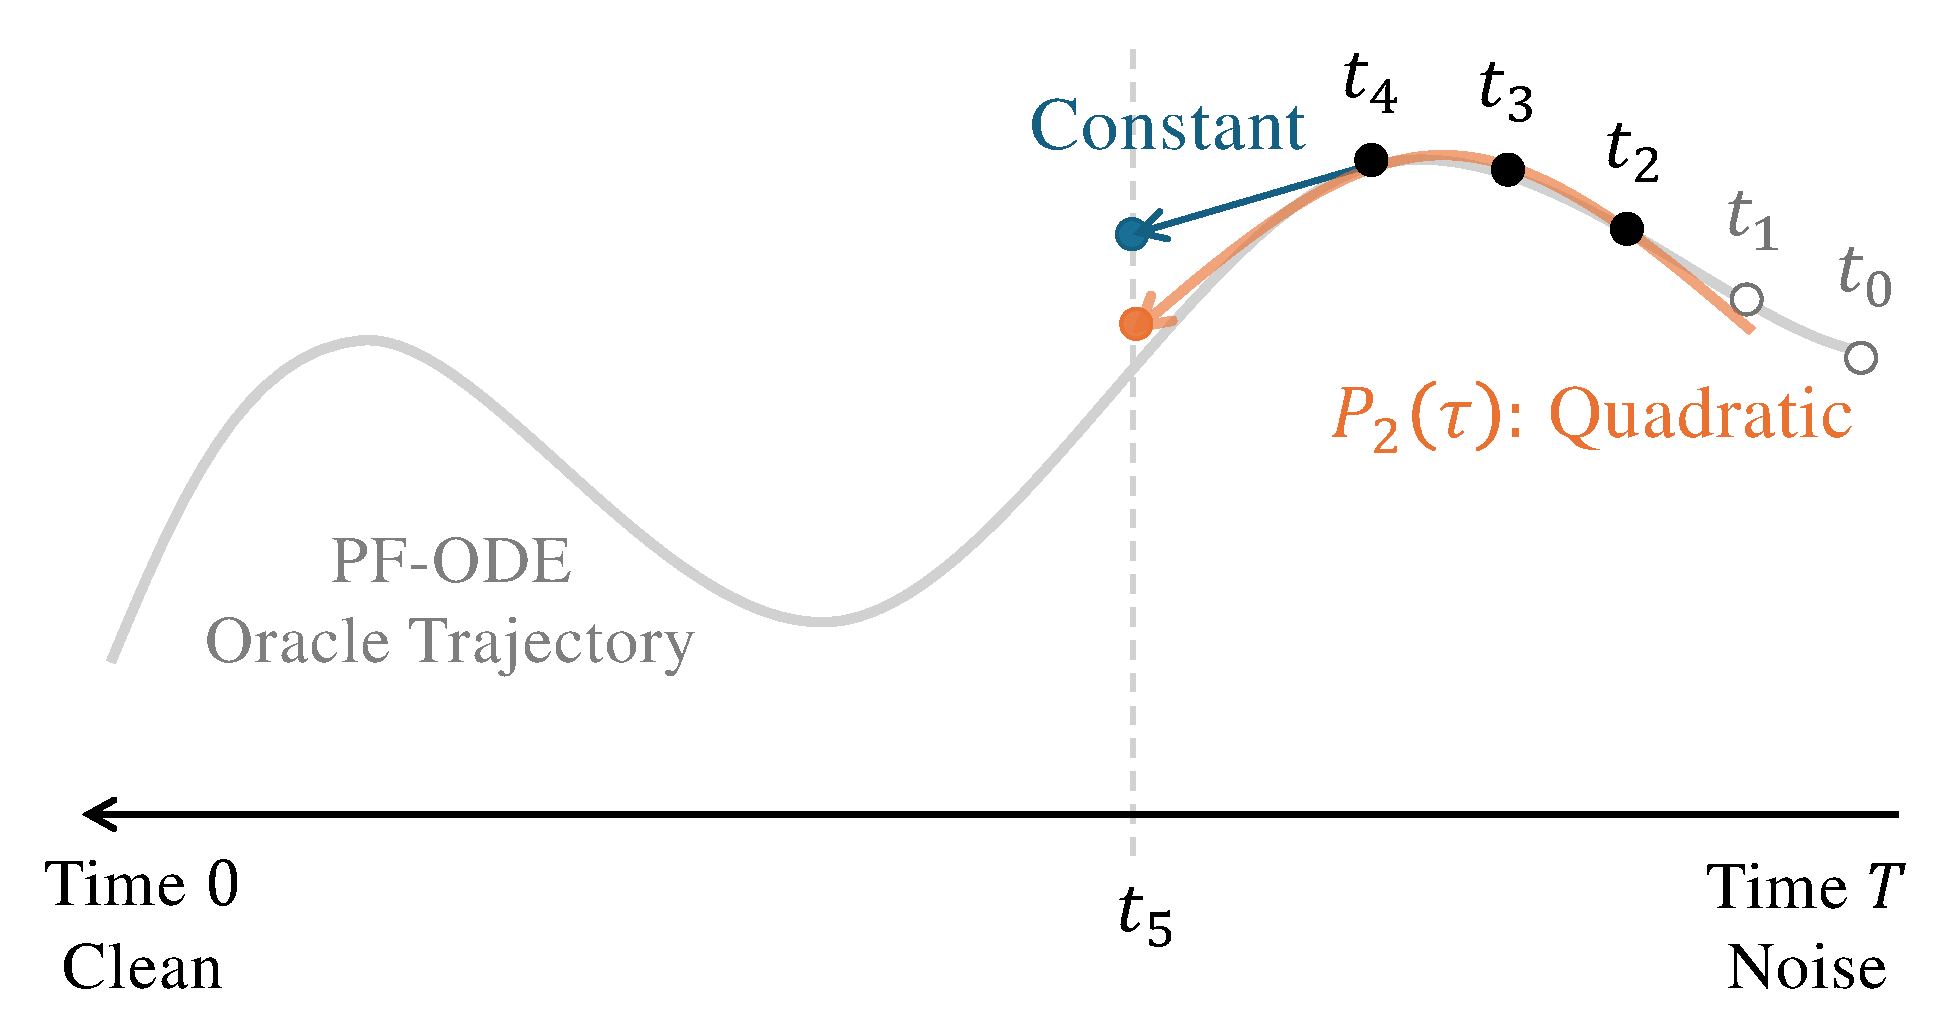
\includegraphics[width=0.85\linewidth]{Images/PartC/DEIS.pdf}
    \caption{\textbfs{Illustration of DEIS as a multistep method.} With three past anchors at
$t_2,t_3,t_4$, DEIS builds a quadratic curve through the model outputs
and extrapolates it over the step from
$t_4$ to $t_5$. The extrapolating polynomial is then integrated against the
known diffusion-dependent weight, capturing variation of the neural prediction
that is neglected by the constant approximation used by DDIM.
\figcredit{Created by the authors.}}
    \label{fig:deis_lagrange}
\end{figure}

A degree-$n$ update needs $n{+}1$ anchors. When they are available
(\emph{sufficient history}, $i \ge n{+}1$), we use the full degree-$n$
scheme. During the initial steps (\emph{insufficient history}, $i \le n$),
we use the highest feasible degree, $i{-}1$, and increase it as more anchors
become available. We treat these two cases below.


\paragraph{Case I: $i = n+1,\dots,M$ (Sufficient History).}
With sufficient history, DEIS reuses the last $n{+}1$ model evaluations as
anchors,
\[
(\tau_j,\rmY_j) := \bigl(t_{i-1-j}, \bm{\epsilon}_{\bm{\phi}^\times}(\tilde{\rvx}_{t_{i-1-j}},t_{i-1-j})\bigr),
\quad j=0,\dots,n.
\]
Viewing
$\tau\mapsto\bm{\epsilon}_{\bm{\phi}^\times}(\rvx_\tau,\tau)$
as a smooth function along the trajectory, we construct the degree-$n$
Lagrange polynomial
\[
P_n(\tau)
= 
\sum_{j=0}^{n}
\underbrace{\Bigl[\prod_{\substack{k=0\\k\neq j}}^{n}
\frac{\tau - t_{i-1-k}}{\,t_{i-1-j} - t_{i-1-k}\,}\Bigr]}_{=:~\ell_j^{(i)}(\tau)}
\bm{\epsilon}_{\bm{\phi}^\times}\bigl(\tilde{\mathbf x}_{t_{i-1-j}}, t_{i-1-j}\bigr)
\]
which by construction satisfies $P_n(\tau_j)=\rmY_j$ for each anchor:
\[
P_n\bigl(\tau_j\bigr)
= \rmY_j =
\bm{\epsilon}_{\bm{\phi}^\times}\bigl(\tilde{\mathbf x}_{t_{i-1-j}}, t_{i-1-j}\bigr),
\quad
 j=0,\ldots,n.
\]
Each $\ell_j^{(i)}$ satisfies
\[
\ell_j^{(i)}\bigl(t_{i-1-m}\bigr)
=
\begin{cases}
1,&m=j,\\
0,&m\neq j.
\end{cases}
\]

The polynomial is then extrapolated beyond the most recent anchor
$t_{i-1}$ over the new step:
\[
\bm{\epsilon}_{\bm{\phi}^\times}(\rvx_\tau,\tau) \approx
P_n(\tau)=\sum_{j=0}^{n}\ell_j^{(i)}(\tau) 
\bm{\epsilon}_{\bm{\phi}^\times}\bigl(\tilde{\rvx}_{t_{i-1-j}}, t_{i-1-j}\bigr), 
\quad \tau \in [t_i,t_{i-1}].
\]
We then substitute $P_n(\tau)$ for
$\beps_{\bm{\phi}^\times}(\rvx_\tau,\tau)$ in the
exponential--integrator formula (\Cref{eq:variation_of_constants}):
\begin{align*}
\int_{t_{i-1}}^{t_i}
\frac{g^2(\tau)}{2\sigma_\tau}
\mathcal{E}(\tau\to t_i)
\beps_{\bm{\phi}^\times}(\rvx_\tau,\tau)\diff\tau
&\approx
\sum_{j=0}^{n}
\underbrace{
\int_{t_{i-1}}^{t_i}
\frac{g^2(\tau)}{2\sigma_\tau}
\mathcal{E}(\tau\to t_i)
\ell_j^{(i)}(\tau)\diff\tau
}_{=:~C_{i,j}}
\\
&\qquad\cdot
\beps_{\bm{\phi}^\times}
(\tilde\rvx_{t_{i-1-j}},t_{i-1-j}).
\end{align*}
The coefficients
\[
C_{i,j}
:=
\frac{1}{2}
\int_{t_{i-1}}^{t_i}
\frac{g^2(\tau)}{\sigma_\tau}
\mathcal{E}(\tau\to t_i)
\ell_j^{(i)}(\tau)\diff\tau
\]
depend only on the noise schedule and the chosen time grid and can therefore
be precomputed. For schedules admitting suitable antiderivatives, these
coefficients are available in closed form; otherwise they can be evaluated
numerically to high accuracy.

Integrating the linear part exactly with
$\mathcal{E}(t_{i-1}\to t_i)$ gives the \emph{AB-DEIS-$n$} update
\[
\tilde\rvx_{t_i}
=
\mathcal{E}(t_{i-1}\to t_i)\tilde\rvx_{t_{i-1}}
+
\sum_{j=0}^{n}
C_{i,j}
\beps_{\bm{\phi}^\times}
(\tilde\rvx_{t_{i-1-j}},t_{i-1-j}).
\]
For the local truncation statements below, let $h$ denote a characteristic
local step size and assume neighboring step ratios remain bounded. Under
standard smoothness assumptions on the model prediction along the empirical
trajectory and regularity of the schedule-dependent weight, the full-history
degree-$n$ construction has formal order $n+1$, with one-step local defect
$\mathcal O(h^{n+2})$.


\paragraph{Case II: $i=1,\dots,n$ (Insufficient History).}
During the initial steps, only $i$ past model evaluations are available.
We therefore use all available anchors and set the polynomial degree to
$i{-}1$:
\[
P_{i-1}(\tau)
=
\sum_{j=0}^{i-1}
\ell_j^{(i)}(\tau) 
\bm{\epsilon}_{\bm{\phi}^\times}\bigl(\tilde{\mathbf x}_{t_{i-1-j}},  t_{i-1-j}\bigr),
\]
where $\ell_j^{(i)}$ is the Lagrange basis of degree $i{-}1$ built on the nodes at time
$\{t_{i-1}, t_{i-2},\ldots,t_{0}\}$. This matches all available anchors and
transitions into the full-history formula once $i\ge n{+}1$.

This is the standard warm-start situation for a multistep method. The first
step uses a constant approximation, the second uses a linear extrapolation,
the third uses a quadratic extrapolation, and so on, until the target degree
$n$ becomes available.


\exm{Special Cases of Lagrange Polynomials}{
\noindent \textbfs{Degree $0$ (one anchor):}
\[
P_0(\tau) = \bm{\epsilon}_{\bm{\phi}^\times}(\tilde\rvx_{t_{i-1}}, t_{i-1}).
\]
This holds the neural prediction fixed at its start-of-step value, exactly as
in the first-order DDIM approximation.

\medskip
\noindent \textbfs{Degree $1$ (two anchors):} the Lagrange polynomial is a linear map passing through the two pre-specified anchors.
\[
P_1(\tau)
= 
\underbrace{\frac{\tau - t_{i-2}}{t_{i-1} - t_{i-2}}}_{\displaystyle \ell_{i-1}(\tau)}
\,\bm{\epsilon}_{\bm{\phi}^\times}(\tilde\rvx_{t_{i-1}}, t_{i-1})
 + 
\underbrace{\frac{\tau - t_{i-1}}{t_{i-2} - t_{i-1}}}_{\displaystyle \ell_{i-2}(\tau)}
\,\bm{\epsilon}_{\bm{\phi}^\times}(\tilde\rvx_{t_{i-2}}, t_{i-2}).
\]
Here $\ell_{i-1}(\tau)$ and $\ell_{i-2}(\tau)$ are the Lagrange basis weights.
They satisfy the interpolation conditions
$P_1(t_{i-1})=\bm{\epsilon}_{\bm{\phi}^\times}(\tilde\rvx_{t_{i-1}}, t_{i-1})$ and
$P_1(t_{i-2})=\bm{\epsilon}_{\bm{\phi}^\times}(\tilde\rvx_{t_{i-2}}, t_{i-2})$,
with
$\ell_{i-1}(\tau)+\ell_{i-2}(\tau)=1$. 
}

\paragraph{Summary of AB-DEIS-$n$ Update.}
Combining the sufficient-history and warm-start cases gives the
\emph{AB-DEIS-$n$} update\footnote{``AB'' refers to the Adams--Bashforth
multistep principle, here applied within the exponential-integrator
formulation~\citep{hochbruck2010exponential}.} Here, $n$ is the target
polynomial degree, using up to $n{+}1$ past evaluations:
\begin{mdframed}
\begin{align*}
\tilde\rvx_{t_i}
= \mathcal{E}(t_{i-1} \to t_i)\,\tilde\rvx_{t_{i-1}}
+ \sum_{j=0}^{\min\{n,\, i-1\}} C_{i,j}\,\beps_{\bm{\phi}^\times}(\tilde\rvx_{t_{i-1-j}},\,t_{i-1-j}),
\end{align*}
with coefficients
\begin{align*}
C_{i,j}
:= \frac{1}{2} \int_{t_{i-1}}^{t_i}
\frac{g^2(\tau)}{\sigma_\tau}\,\mathcal{E}(\tau \to t_i)\,
\Bigg[\prod_{\substack{k=0\\k\neq j}}^{\min\{n,\, i-1\}}
\frac{\tau - t_{i-1-k}}{\,t_{i-1-j} - t_{i-1-k}\,}\Bigg]\,d\tau.
\end{align*}
\end{mdframed}

When $i\ge n{+}1$ (sufficient history), $\min\{n,\,i-1\}=n$, and the
full-history degree-$n$ step has one-step local truncation error
$\mathcal O(h^{n+2})$ under the assumptions above, corresponding
to a method of order $n+1$.

During warm start ($i\le n$), the degree is $i-1$, so the
one-step local truncation error is $\mathcal O(h^{i+1})$, and the corresponding
step is formally of order $i$. Thus, the order increases from $1$ at the first
step and reaches the full order $n+1$ once $n+1$ anchors are available.
As with standard multistep methods, lower-order warm-start steps do not by
themselves establish a global order-$(n+1)$ guarantee; such a guarantee also
requires stability and starting values of sufficient accuracy.

Very large $n$ can degrade numerical behavior because high-degree
extrapolation becomes increasingly sensitive to the spacing of the anchors,
errors in the stored model predictions, and stability considerations.
Relatively small polynomial degrees are therefore preferred in practice.

As we will see in the following subsection, the special case $n{=}0$ reduces
exactly to deterministic DDIM, i.e., the first-order factored
exponential-integrator update.
\subsection{DDIM = AB-DEIS-0}
\label{sec:ddim-deis}

The connection to DDIM becomes immediate at degree $n=0$. In this case, the
Lagrange polynomial is constant, so DEIS uses only the most recent model
prediction throughout the next step. The corresponding coefficient simplifies
to
\[
C_{i0} = \frac{1}{2} \int_{t_{i-1}}^{t_{i}} \frac{g^2(\tau)}{\sigma_\tau} \mathcal{E}(\tau \shortrightarrow t_i)   \mathrm{d}\tau.
\]
Substituting into the update formula yields the zeroth-order AB-DEIS scheme:
\begin{align}\label{eq:deis-0}
  \tilde\rvx_{t_{i}} &=  \mathcal{E}(t_{i-1} \shortrightarrow t_{i})\tilde\rvx_{t_{i-1}} + C_{i0} \bm{\epsilon}_{\bm{\phi}^\times}(\tilde\rvx_{t_{i-1}}, t_{i-1})\nonumber\\
  &=e^{\int_{t_{i-1}}^{t_{i}}f(u)\diff u} \tilde\rvx_{t_{i-1}} + \Big( \int_{t_{i-1}}^{t_{i}} \frac{g^2(\tau)}{2\sigma_\tau} e^{\int_{\tau}^{t_{i}}f(u)\diff u}   \mathrm{d}\tau
\Big) \bm{\epsilon}_{\bm{\phi}^\times}(\tilde\rvx_{t_{i-1}}, t_{i-1}).  
\end{align}
This is exactly the same first-order factored approximation used by
deterministic DDIM: the neural prediction is held fixed at
$t_{i-1}$, while the known integrating factor and schedule-dependent
coefficient remain inside the integral and are propagated over the full step.
Hence, AB-DEIS-0 and DDIM are not merely first-order equivalent; they give
the same finite-step update.

\proppnp{DDIM = AB-DEIS-0}{ddim-deis}{\Cref{eq:deis-0} is identical to the DDIM update in \Cref{eq:ddim-euler}.}

This also clarifies the role of DEIS in the solver hierarchy. We remark that the index
``$0$'' refers to the \emph{polynomial degree}, not the numerical order:
AB-DEIS-0 is still a first-order method. Higher-degree DEIS keeps the same
analytic treatment of the known diffusion dynamics but replaces this constant
prediction by polynomial extrapolation from additional past model evaluations.
Thus, DDIM is the degree-zero base case from which the DEIS multistep
construction naturally extends.

Later, in \Cref{subsec:dpm-solver++-multi}, we will encounter another route to
a multistep diffusion solver; that is, DPM-Solver\texttt{++}(2M). It starts from a local
Taylor expansion of the data prediction in log-SNR time and recycles previous
model evaluations through a backward finite difference to estimate the required
derivative. Although its representation and derivation differ from those of
DEIS, both methods use past model evaluations to capture the variation of the
neural prediction without introducing additional within-step stages. We return
to this connection in \Cref{subsec:dpm-deis}, where we compare the two
constructions more explicitly.
    
\clearpage
\newpage



\section{\texorpdfstring{DPM-Solver}{DPM-Solver}}\label{sec:dpm}

DPM-Solver~\citep{lu2022dpm} develops higher-order solvers for the empirical
PF-ODE by exploiting the same diffusion-specific structure that appeared in
our discussion of DDIM. The central goal is to obtain accurate samples using
far fewer neural-network evaluations than a first-order sampler. The original
DPM-Solver focuses on noise prediction and constructs first-, second-, and
third-order single-step solvers; later extensions, including
DPM-Solver\texttt{++}~\citep{lu2022dpm2} and
DPM-Solver-v3~\citep{zheng2023dpm}, further develop this family.

\paragraph{High-Level Idea of DPM-Solver.}
The DDIM discussion in \Cref{sec:revisit-ddim} showed that, under
$\beps$-prediction, a first-order update can be obtained by retaining the
known diffusion schedule analytically while holding the neural prediction
fixed over each step,
\[
\beps_{\bm{\phi}^\times}(\rvx_\tau,\tau)
\approx
\beps_{\bm{\phi}^\times}(\tilde\rvx_s,s).
\]
DPM-Solver~\citep{lu2022dpm} builds naturally on this idea: rather than
treating the neural prediction as constant, it seeks higher-order
approximations of how the prediction varies along the trajectory. Like DEIS,
it starts from the semilinear $\beps$-prediction form of the PF-ODE,
\begin{align}
\label{eq:noise-alpha-sigma}
\frac{\diff \rvx_t}{\diff t}
=
\frac{\alpha_t'}{\alpha_t}\rvx_t
-
\sigma_t
\left(
\frac{\alpha_t'}{\alpha_t}
-
\frac{\sigma_t'}{\sigma_t}
\right)
\beps_{\bphi^\times}(\rvx_t,t),
\end{align}
and its variation-of-constants representation introduced in the Prologue.
Its key additional ingredient is to reparameterize time by the
\emph{half-log signal-to-noise ratio}, following the log-SNR
parameterization of VDM~\citep{kingma2021variational},
\begin{align}
\label{eq:lambda}
\lambda_t
:=
\log\frac{\alpha_t}{\sigma_t}.
\end{align}
This coordinate is directly related to DDIM's schedule-aligned clock
$\rho_t=\sigma_t/\alpha_t$ (discussed around \Cref{eq:ddim-coordinate-ode-t}) through $\rho_t=e^{-\lambda_t}$, and turns the
remaining model-dependent term into a particularly convenient exponentially
weighted integral. Local Taylor approximations of the neural prediction in
$\lambda$ can then be integrated analytically, providing a systematic route
from the first-order DDIM update to higher-order diffusion solvers.


\subsection{DPM-Solver's Insight: Time Reparameterization via Log-SNR}
\label{subsec:dpm-method}   

We now make the log-SNR reparameterization in \Cref{eq:lambda} precise and
derive the corresponding PF-ODE representation.

\paragraph{Change-of-Variable to Log-SNR in PF-ODE.}
Suppose that $\alpha_t>0$, $\sigma_t>0$, and the log-SNR coordinate
$\lambda_t$ in \Cref{eq:lambda} is strictly monotone on the interval of
interest. It then admits an inverse function $t_\lambda(\cdot)$ satisfying
\[
t=t_\lambda(\lambda(t)).
\]
For schedules with $\sigma_0=0$, one has $\lambda_t\to+\infty$ as
$t\to0$, so formulas involving the endpoint $t=0$ are understood through
the corresponding limit or through a small positive terminal time in a
numerical implementation.

We then express the state, schedule, and neural prediction in the
$\lambda$-coordinate. A hat ($\hat{\cdot}$) together with $\lambda$ indicates that the corresponding quantity is
viewed in this reparameterized time coordinate. More precisely, define
\begin{align}
\begin{aligned}
\label{eq:change-of-var-x-epsilon}
\hat{\rvx}_{\lambda}
&:=
\rvx_{t_\lambda(\lambda)},
\\
\alpha_\lambda
&:=
\alpha_{t_\lambda(\lambda)},
\qquad
\sigma_\lambda
:=
\sigma_{t_\lambda(\lambda)},
\\
\hat{\bm{\epsilon}}_{\bm{\phi}^\times}(\rvx,\lambda)
&:=
\bm{\epsilon}_{\bm{\phi}^\times}
\bigl(
\rvx,
t_\lambda(\lambda)
\bigr).
\end{aligned}
\end{align}
Hence, along the empirical PF-ODE trajectory,
\[
\hat{\bm{\epsilon}}_{\bm{\phi}^\times}
(\hat\rvx_\lambda,\lambda)
=
\bm{\epsilon}_{\bm{\phi}^\times}
\bigl(
\rvx_{t_\lambda(\lambda)},
t_\lambda(\lambda)
\bigr).
\]
Since
\[
\frac{\diff\lambda_t}{\diff t}
=
\frac{\alpha_t'}{\alpha_t}
-
\frac{\sigma_t'}{\sigma_t},
\]
the PF-ODE in \Cref{eq:noise-alpha-sigma} can be written as
\[
\frac{\diff\rvx_t}{\diff t}
=
\frac{\diff\log\alpha_t}{\diff t}\rvx_t
-
\sigma_t
\frac{\diff\lambda_t}{\diff t}
\bm{\epsilon}_{\bm{\phi}^\times}(\rvx_t,t).
\]
Applying the chain rule,
\[
\frac{\diff\rvx_t}{\diff t}
=
\frac{\diff\hat\rvx_\lambda}{\diff\lambda}
\frac{\diff\lambda_t}{\diff t},
\qquad
\frac{\diff\log\alpha_t}{\diff t}
=
\frac{\diff\log\alpha_\lambda}{\diff\lambda}
\frac{\diff\lambda_t}{\diff t},
\]
gives the PF-ODE in log-SNR time:
\begin{mdframed}
\begin{align}
\label{eq:diffusion_ode_lambda_eps}
\frac{\diff\hat{\rvx}_\lambda}{\diff\lambda}
=
\frac{\diff\log\alpha_\lambda}{\diff\lambda}
\hat{\rvx}_\lambda
-
\sigma_\lambda
\hat{\bm{\epsilon}}_{\bm{\phi}^\times}
(\hat{\rvx}_\lambda,\lambda).
\end{align}
\end{mdframed}

Applying the same exponential-integrator (variation-of-constants) technique
to \Cref{eq:diffusion_ode_lambda_eps} gives the following exact solution.

\proppp{Exponentially Weighted Exact Solution}{exp-wgt-exact-sol}{
Given an initial value $\rvx_s$ at time $s>0$, the exact empirical PF-ODE
solution $\widetilde\bPsi_{s\to t}(\rvx_s)$ at time $t\in(0,s]$ can be
re-expressed as
\begin{equation}
\label{eq:analytic_solution}
\widetilde\bPsi_{s\to t}(\rvx_s)
=
\frac{\alpha_t}{\alpha_s}\rvx_s
-
\alpha_t
\int_{\lambda_s}^{\lambda_t}
e^{-\lambda}
\hat{\bm{\epsilon}}_{\bm{\phi}^\times}
(\hat\rvx_\lambda,\lambda)
\diff\lambda.
\end{equation}
When the endpoint satisfies $\sigma_0=0$, the case $t=0$ is understood
through the corresponding limit.
}{
From \Cref{eq:diffusion_ode_lambda_eps}, the integrating factor associated
with the linear term satisfies
\[
\exp\left(
\int_{\lambda_s}^{\lambda_t}
\frac{\diff\log\alpha_\lambda}{\diff\lambda}
\diff\lambda
\right)
=
\frac{\alpha_t}{\alpha_s}.
\]
Therefore, the variation-of-constants formula gives
\begin{align*}
\widetilde\bPsi_{s\to t}(\rvx_s)
&=
\frac{\alpha_t}{\alpha_s}\rvx_s
-
\int_{\lambda_s}^{\lambda_t}
\frac{\alpha_t}{\alpha_\lambda}
\sigma_\lambda
\hat{\bm{\epsilon}}_{\bm{\phi}^\times}
(\hat\rvx_\lambda,\lambda)
\diff\lambda
\\
&=
\frac{\alpha_t}{\alpha_s}\rvx_s
-
\alpha_t
\int_{\lambda_s}^{\lambda_t}
e^{-\lambda}
\hat{\bm{\epsilon}}_{\bm{\phi}^\times}
(\hat\rvx_\lambda,\lambda)
\diff\lambda,
\end{align*}
where the last equality follows from
$\sigma_\lambda/\alpha_\lambda=e^{-\lambda}$.
}

The key numerical consequence is now explicit. In $\lambda$-time, the only
model-dependent quantity in the exact solution appears inside
\[
\int_{\lambda_s}^{\lambda_t}
e^{-\lambda}
\hat{\bm{\epsilon}}_{\bm{\phi}^\times}
(\hat\rvx_\lambda,\lambda)\diff\lambda.
\]
When the model output is locally approximated by a Taylor polynomial in
$\lambda$, the resulting exponentially weighted polynomial terms can be
integrated in closed form, yielding explicit higher-order update
coefficients. Thus, as in the factored viewpoint of the Prologue, the known
schedule dependence is retained analytically while the approximation is
concentrated on the neural prediction.

\paragraph{Intuition of Why Reparameterize Time?}
For strictly monotone $\lambda(t)$, a local first-order change of variables gives
\[
|\Delta t|
\approx
\frac{|\Delta\lambda|}{|\lambda'(t)|}.
\]
Thus, if the numerical grid uses a fixed step size $|\Delta\lambda|$, the
induced step in $t$ is smaller where $|\lambda'(t)|$ is larger
(i.e., where $\lambda$ changes rapidly with $t$), and larger where
$|\lambda'(t)|$ is smaller.

The reparameterization itself does not alter the PF-ODE solution path; it only
changes how the same path is parameterized:
\[
\frac{\diff \hat\rvx_\lambda}{\diff \lambda}
=
\frac{1}{\lambda'(t)}
\frac{\diff \rvx_t}{\diff t}.
\]
Hence, where $|\lambda'(t)|$ is large, the same change of the trajectory with
respect to $t$ is represented over a larger range of $\lambda$.

More importantly, $\lambda(t)$ measures progress through the diffusion process
directly in terms of the relative balance between signal and noise. A fixed
$\Delta\lambda$ corresponds to a fixed multiplicative change in
$\alpha_t/\sigma_t$, or equivalently to a fixed additive change in log-SNR,
whereas the same $\Delta t$ may correspond to very different changes in
corruption level at different times. Therefore, choosing numerical nodes
uniformly in $\lambda$ provides a natural way to redistribute resolution along
the diffusion trajectory. The precise induced spacing in the original time
variable $t$ depends on the chosen noise schedule. Two simple examples
illustrate this effect:

\begin{itemize}
\item \textbfs{$(\alpha_t,\sigma_t)=(1-t,t)$.}
This corresponds to the linear interpolation commonly used in flow matching.
Then
\[
\lambda(t)
=
\log\frac{1-t}{t},
\qquad
\lambda'(t)
=
-\frac{1}{t(1-t)},
\]
so locally
\[
|\Delta t|
\approx
|\Delta\lambda|\,t(1-t).
\]
Hence, a uniform grid in $\lambda$ induces very small steps in $t$ near both
endpoints $t\to0$ and $t\to1$, and larger steps around the middle of the
trajectory.

\item \textbfs{$(\alpha_t,\sigma_t)=(1,t)$.}
This corresponds to the EDM parameterization~\citep{karras2022elucidating}
when the independent variable $t$ is taken directly as the noise level
$\sigma_t$. Then
\[
\lambda(t)
=
\log\frac{1}{t},
\qquad
\lambda'(t)
=
-\frac{1}{t},
\]
and therefore
\[
|\Delta t|
\approx
|\Delta\lambda|\,t.
\]
In fact, uniform spacing in $\lambda$ implies
\[
t=e^{-\lambda},
\]
so the corresponding noise levels are geometrically spaced. Thus, the grid
contains finer absolute spacing at small noise levels (high SNR) and coarser
absolute spacing at large noise levels (low SNR).
\end{itemize}



\subsection{Estimating the Integral with Taylor Expansion}\label{subsec:dpm-method-2} 
DEIS and DPM-Solver exploit the same factored principle but obtain
higher-order information in different ways. DEIS reuses predictions from
previous completed steps to extrapolate the neural prediction over the next
interval. DPM-Solver instead works in the log-SNR coordinate $\lambda$ and
uses a local Taylor expansion of the neural prediction, with the required
higher-order information obtained from additional evaluations within the
current step. We now derive this single-step construction.

From \Cref{eq:analytic_solution}, the exact empirical PF-ODE flow initialized
at the current numerical state $\tilde\rvx_s$ is
\begin{equation}
\label{eqn:analytic_solution_each_step}
\widetilde\bPsi_{s\to t}(\tilde\rvx_s)
=
\frac{\alpha_t}{\alpha_s}\tilde\rvx_s
-
\alpha_t
\int_{\lambda_s}^{\lambda_t}
e^{-\lambda}
\hat{\bm{\epsilon}}_{\bm{\phi}^\times}
(\hat\rvx_\lambda,\lambda)
\diff\lambda,
\end{equation}
where
$\hat\rvx_{\lambda_s}=\tilde\rvx_s$ and
$\hat\rvx_\lambda$ denotes the corresponding exact empirical PF-ODE
trajectory over the current step. Therefore, after the known
schedule-dependent factors have been handled analytically, the remaining
numerical problem is to approximate
\[
\lambda
\longmapsto
\hat{\bm{\epsilon}}_{\bm{\phi}^\times}
(\hat\rvx_\lambda,\lambda)
\]
inside the weighted integral.

For $n\geq1$, we expand this neural prediction about $\lambda_s$:
\begin{equation*}
\hat{\bm{\epsilon}}_{\bm{\phi}^\times}
(\hat\rvx_\lambda,\lambda)
=
\sum_{k=0}^{n-1}
\frac{(\lambda-\lambda_s)^k}{k!}
\hat{\bm{\epsilon}}_{\bm{\phi}^\times}^{(k)}
(\hat\rvx_{\lambda_s},\lambda_s)
+
\mathcal O\bigl((\lambda-\lambda_s)^n\bigr),
\end{equation*}
where
\[
\hat{\bm{\epsilon}}_{\bm{\phi}^\times}^{(k)}
(\hat\rvx_\lambda,\lambda)
:=
\frac{\diff^k}{\diff\lambda^k}
\hat{\bm{\epsilon}}_{\bm{\phi}^\times}
(\hat\rvx_\lambda,\lambda)
\]
denotes the $k$-th \emph{total derivative along the empirical PF-ODE
trajectory}. In particular,
\[
\frac{\diff}{\diff\lambda}
\hat{\bm{\epsilon}}_{\bm{\phi}^\times}
(\hat\rvx_\lambda,\lambda)
=
\frac{\partial}{\partial\lambda}
\hat{\bm{\epsilon}}_{\bm{\phi}^\times}
(\hat\rvx_\lambda,\lambda)
+
J_{\rvx}
\hat{\bm{\epsilon}}_{\bm{\phi}^\times}
(\hat\rvx_\lambda,\lambda)
\frac{\diff\hat\rvx_\lambda}{\diff\lambda},
\]
so the derivative includes both the explicit dependence on $\lambda$ and the
dependence through the evolving state.

Substituting the Taylor expansion into
\Cref{eqn:analytic_solution_each_step} gives
\begin{mdframed}
\begin{equation}
\label{eq:k-th-expansion}
\widetilde\bPsi_{s\to t}(\tilde\rvx_s)
=
\frac{\alpha_t}{\alpha_s}\tilde\rvx_s
-
\alpha_t
\sum_{k=0}^{n-1}
{\color{cyan}
\hat{\bm{\epsilon}}_{\bm{\phi}^\times}^{(k)}
(\hat\rvx_{\lambda_s},\lambda_s)}
\,{\color{orange}C_k}
+
\mathcal O(h^{n+1}),
\end{equation}
where
\[
h:=\lambda_t-\lambda_s,
\qquad
{\color{orange}C_k}
:=
\int_{\lambda_s}^{\lambda_t}
e^{-\lambda}
\frac{(\lambda-\lambda_s)^k}{k!}
\diff\lambda.
\]
The coefficients ${\color{orange}C_k}$ depend only on the log-SNR interval
and can be evaluated analytically.
\end{mdframed}

If the required trajectory derivatives were available, dropping the
$\mathcal O(h^{n+1})$ remainder would give the corresponding formal
$n$-th order update. DPM-Solver avoids explicitly differentiating the neural
network by approximating these derivatives from additional model evaluations,
as described in the next subsection.

\exm{DPM-Solver-1}{
For $n=1$, the exact empirical flow satisfies
\[
\widetilde\bPsi_{s\to t}(\tilde\rvx_s)
=
\frac{\alpha_t}{\alpha_s}\tilde\rvx_s
-
\sigma_t
\left(e^h-1\right)
\bm{\epsilon}_{\bm{\phi}^\times}(\tilde\rvx_s,s)
+
\mathcal O(h^2).
\]
Dropping the $\mathcal O(h^2)$ remainder defines
DPM-Solver-1:
\begin{align}
\label{eq:dpm-1}
\tilde\rvx_t^{\mathrm{DPM\text{-}Solver\text{-}1}}
:=
\frac{\alpha_t}{\alpha_s}\tilde\rvx_s
-
\sigma_t
\left(e^h-1\right)
\bm{\epsilon}_{\bm{\phi}^\times}(\tilde\rvx_s,s).
\end{align}
This finite-step update is exactly the deterministic DDIM update, as shown
in \Cref{subsec:ddim=dpm-solver-1}.
}

DPM-Solver-$n$ with $n \geq 2$ requires evaluating the $k^{\text{th}}$-derivative {\color{cyan}$\hat{\bm{\epsilon}}_{\bm{\phi}^\times}^{(k)}(\hat\rvx_\lambda, \lambda)$} for $k \leq n-1$. However, directly computing higher-order derivatives is computationally expensive in practice. \citet{lu2022dpm} also propose efficient approximation methods for these derivatives, which will be detailed in the next subsection.

 
\subsection{Implementation of DPM-Solver-$n$}\label{subsec:dpm-n-method} 

\paragraph{DPM-Solver-$n$ with $n \geq 2$.}
In practice, implementing a higher-order DPM-Solver-$n$ entails the following:
\begin{itemize}
    \item Precomputing the coefficients ${\color{orange}C_k}$;
    \item Approximating the $k^{\text{th}}$ derivative {\color{cyan}$\hat{\bm{\epsilon}}_{\bm{\phi}^\times}^{(k)}(\hat\rvx_\lambda,\lambda)$} for $k \leq n-1$ to circumvent the costly computation of exact higher-order derivatives—a challenge well-studied in the ODE literature~\citep{hochbruck2005explicit,luan2021efficient}. One common strategy is finite difference approximation.
\end{itemize}

We now elaborate on the first two points.


\subparagraph{Precomputing ${\color{orange}C_k}$.}
Let $s$ and $t$ denote the start and end times, respectively, and define
$h:=\lambda_t-\lambda_s$. The Taylor expansion of the exact empirical
PF-ODE flow takes the form
\begin{equation}
\label{eq:analytic_expansion}
\widetilde\bPsi_{s\to t}(\rvx_s)
=
\frac{\alpha_t}{\alpha_s}\rvx_s
-
\sigma_t
\sum_{k=0}^{n-1}
h^{k+1}
\varphi_{k+1}(h)
\hat{\bm{\epsilon}}_{\bm{\phi}^\times}^{(k)}
(\hat\rvx_{\lambda_s},\lambda_s)
+
\mathcal O(h^{n+1}),
\end{equation}
where, for $m\geq1$,
\[
\varphi_m(h)
:=
\frac{
e^h-\sum_{j=0}^{m-1}\frac{h^j}{j!}
}{
h^m
},
\qquad
\varphi_m(0):=\frac{1}{m!}.
\]
For the first three cases,
\begin{align*}
\varphi_1(h)
&=
\frac{e^h-1}{h},
&
\varphi_2(h)
&=
\frac{e^h-h-1}{h^2},
&
\varphi_3(h)
&=
\frac{e^h-\frac{h^2}{2}-h-1}{h^3}.
\end{align*}

\exm{Third-Order Expansion with Exact Derivatives}{
For $n=3$, \Cref{eq:analytic_expansion} becomes
\begin{equation}
\label{eq:example-dpm-solver-3-exact}
\begin{aligned}
\widetilde\bPsi_{s\to t}(\rvx_s)
=
\frac{\alpha_t}{\alpha_s}\rvx_s
&-
\sigma_t
\left(e^h-1\right)
\hat{\bm{\epsilon}}_{\bm{\phi}^\times}
(\hat\rvx_{\lambda_s},\lambda_s)
\\
&-
\sigma_t
\left(e^h-h-1\right)
\hat{\bm{\epsilon}}_{\bm{\phi}^\times}^{(1)}
(\hat\rvx_{\lambda_s},\lambda_s)
\\
&-
\sigma_t
\left(
e^h-\frac{h^2}{2}-h-1
\right)
\hat{\bm{\epsilon}}_{\bm{\phi}^\times}^{(2)}
(\hat\rvx_{\lambda_s},\lambda_s)
+
\mathcal O(h^4).
\end{aligned}
\end{equation}
}



\subparagraph{Approximating {\color{cyan}$\hat{\bm{\epsilon}}_{\bm{\phi}^\times}^{(k)}(\hat\rvx_\lambda,\lambda)$} for $k \leq n-1$.}
For $n \geq 2$, following the standard approach of single-step ODE
solvers~\citep{atkinson2009numerical}, \citet{lu2022dpm} use additional model
evaluations within the current step to approximate the higher-order
derivatives. We illustrate this idea for $n=2$.

Let $\gamma\in(0,1]$ specify a stage point in the log-SNR interval
$[\lambda_s,\lambda_t]$. Given an estimate $\tilde\rvx_s$ at $s$, define
\[
s^{\mathrm{mid}}
=
t_\lambda\left(\lambda_s+\gamma h\right),
\qquad
h:=\lambda_t-\lambda_s.
\]
For $\gamma\in(0,1)$ this is an interior point, while $\gamma=1$ corresponds
to the endpoint $t$. We first use a DPM-Solver-1 step to predict the state at
this stage:
\[
\rvx^{\mathrm{mid}}
=
\frac{\alpha_{s^{\mathrm{mid}}}}{\alpha_s}\tilde\rvx_s
-
\sigma_{s^{\mathrm{mid}}}
\left(e^{\gamma h}-1\right)
\bm{\epsilon}_{\bm{\phi}^\times}(\tilde\rvx_s,s).
\]
The difference between the model predictions at the starting and stage points
then provides a finite-difference approximation of the first total derivative
along the trajectory:
\[
\hat{\bm{\epsilon}}_{\bm{\phi}^\times}^{(1)}
(\hat\rvx_{\lambda_s},\lambda_s)
\approx
\frac{
\bm{\epsilon}_{\bm{\phi}^\times}
(\rvx^{\mathrm{mid}},s^{\mathrm{mid}})
-
\bm{\epsilon}_{\bm{\phi}^\times}
(\tilde\rvx_s,s)
}{
\gamma h
}.
\]
Substituting this approximation into the second-order expansion gives
\begin{align}
\label{eq:dpm-solver-2-app}
\begin{aligned}
\widetilde\bPsi_{s\to t}(\tilde\rvx_s)
=
\frac{\alpha_t}{\alpha_s}\tilde\rvx_s
&-
\sigma_t
\left(e^h-1\right)
\bm{\epsilon}_{\bm{\phi}^\times}(\tilde\rvx_s,s)
\\
&-
\frac{\sigma_t}{\gamma h}
\left(e^h-h-1\right)
\left[
\bm{\epsilon}_{\bm{\phi}^\times}
(\rvx^{\mathrm{mid}},s^{\mathrm{mid}})
-
\bm{\epsilon}_{\bm{\phi}^\times}
(\tilde\rvx_s,s)
\right]
+
\mathcal O(h^3).
\end{aligned}
\end{align}
Thus, dropping the $\mathcal O(h^3)$ remainder yields a second-order
single-step update.

For the midpoint choice $\gamma=\tfrac12$, DPM-Solver-2 admits the simpler
two-stage form in \Cref{alg:dpm-solver-2}. This update differs from
\Cref{eq:dpm-solver-2-app} only by $\mathcal O(h^3)$ and therefore has the
same second-order accuracy.
\begin{algorithm}[H]
    \centering
    \caption{DPM-Solver-2 (with $\gamma=\tfrac12$).}
    \label{alg:dpm-solver-2}
    \begin{algorithmic}[1]
    \Require initial value $\rvx_T$, time steps $\{t_i\}_{i=0}^M$, model ${\bm{\epsilon}}_{\bm{\phi}^\times}$
        \State $\tilde\rvx_{t_0}\gets\rvx_T$
        \For{$i\gets 1$ to $M$}
        \State $h_i \gets \lambda_{t_i}-\lambda_{t_{i-1}}$
        \State $s_i^{\mathrm{mid}}
        \gets
        t_\lambda\left(
        \tfrac{\lambda_{t_{i-1}}+\lambda_{t_i}}{2}
        \right)$
        \State
        $\rvx_i^{\mathrm{mid}}
        \gets
        \tfrac{\alpha_{s_i^{\mathrm{mid}}}}{\alpha_{t_{i-1}}}
        \tilde\rvx_{t_{i-1}}
        -
        \sigma_{s_i^{\mathrm{mid}}}
        \left(e^{h_i/2}-1\right)
        {\bm{\epsilon}}_{\bm{\phi}^\times}
        (\tilde\rvx_{t_{i-1}},t_{i-1})$
        \State
        $\tilde\rvx_{t_i}
        \gets
        \tfrac{\alpha_{t_i}}{\alpha_{t_{i-1}}}
        \tilde\rvx_{t_{i-1}}
        -
        \sigma_{t_i}
        \left(e^{h_i}-1\right)
        {\bm{\epsilon}}_{\bm{\phi}^\times}
        (\rvx_i^{\mathrm{mid}},s_i^{\mathrm{mid}})$
        \EndFor
        \State \Return $\tilde\rvx_{t_M}$
    \end{algorithmic}
\end{algorithm}

\rmkb{
The finite difference above approximates the \emph{total} $\lambda$-derivative
of the neural prediction along the empirical PF-ODE trajectory. Under standard
smoothness assumptions,
\[
\frac{
\bm{\epsilon}_{\bm{\phi}^\times}
(\rvx^{\mathrm{mid}},s^{\mathrm{mid}})
-
\bm{\epsilon}_{\bm{\phi}^\times}
(\tilde\rvx_s,s)
}{
\gamma h
}
=
\hat{\bm{\epsilon}}_{\bm{\phi}^\times}^{(1)}
(\hat\rvx_{\lambda_s},\lambda_s)
+
\mathcal O(h).
\]
Here, the intermediate state is itself obtained by a first-order
DPM-Solver-1 step, whose stage error is $\mathcal O(h^2)$; under smoothness
of the model, this does not change the $\mathcal O(h)$ accuracy of the
difference quotient.

In \Cref{eq:dpm-solver-2-app}, this derivative approximation is multiplied by
\[
e^h-h-1=\mathcal O(h^2),
\]
so its induced error is $\mathcal O(h^3)$. Hence, the resulting method is
second-order accurate for any fixed $\gamma\in(0,1]$.

This single-step construction uses two model evaluations: one at
$(\tilde\rvx_s,s)$ and one at the predicted stage
$(\rvx^{\mathrm{mid}},s^{\mathrm{mid}})$. The choice of $\gamma$ does not
change the formal second-order accuracy, but it changes the stage location
and the error constant. In particular, $\gamma=\tfrac12$ places the second
evaluation at the midpoint of the log-SNR interval, giving the commonly used
midpoint version of DPM-Solver-2.
}

\paragraph{Implementation Detail: Selection of Sampling Timesteps.}
Since DPM-Solver constructs its local high-order approximation in log-SNR time
$\lambda$, a natural choice is to place the numerical nodes uniformly in
$\lambda$. For a finite terminal time $t_M>0$, this gives
\[
\lambda_{t_i}
=
\lambda_{t_0}
+
\frac{i}{M}
\left(
\lambda_{t_M}-\lambda_{t_0}
\right),
\qquad
i=0,\ldots,M.
\]
If $\sigma_0=0$, then $\lambda_0=+\infty$, so in practice one instead uses a
finite terminal log-SNR corresponding to a small positive time, with the
endpoint handled by the corresponding limiting or final denoising step.


Although the derivation is carried out in $\lambda$-space, the pre-trained
model and schedule $(\alpha_t,\sigma_t)$ are usually parameterized by the
original diffusion time $t$. During sampling, each selected log-SNR node is
therefore mapped back through
\[
t_i=t_\lambda(\lambda_{t_i})
\]
whenever the model is evaluated or the schedule coefficients are required;
see, for example, \Cref{alg:dpm-solver-2}. Thus, $\lambda$ serves as the
numerical integration coordinate, while the sampler continues to evaluate
the original pre-trained diffusion model at its corresponding time labels.



\subsection{DDIM $=$ DPM-Solver-1}
\label{subsec:ddim=dpm-solver-1}

The first-order DPM-Solver recovers DDIM exactly. Both methods start from an
exact integral representation of the same noise-prediction PF-ODE and make
the same approximation over one step:
\[
\beps_{\bm{\phi}^\times}(\rvx_\tau,\tau)
\approx
\beps_{\bm{\phi}^\times}(\tilde\rvx_s,s).
\]
The remaining schedule-dependent terms are then integrated analytically.
DDIM applies this construction directly in the schedule-aligned form derived
earlier, whereas DPM-Solver first rewrites the integral using the log-SNR
coordinate
\[
\lambda_t
=
\log\frac{\alpha_t}{\sigma_t}.
\]
At first order, this change of numerical clock does not alter the constant
approximation of the model prediction. Consequently, the two derivations
produce exactly the same finite-step update.

\proppp{DDIM is DPM-Solver-1}{ddim-dpm}{
For a fixed diffusion schedule $(\alpha_t,\sigma_t)$, the deterministic DDIM
update in \Cref{eq:ddim-euler} is identical to the DPM-Solver-1 update in
\Cref{eq:dpm-1}.
}{
By the definition of $\lambda$,
\[
\frac{\sigma_s}{\alpha_s}
=
e^{-\lambda_s},
\qquad
\frac{\sigma_t}{\alpha_t}
=
e^{-\lambda_t}.
\]
Let
\[
h
=
\lambda_t-\lambda_s.
\]
Then
\[
e^h
=
\frac{\alpha_t/\sigma_t}{\alpha_s/\sigma_s}
=
\frac{\alpha_t\sigma_s}{\sigma_t\alpha_s},
\]
and therefore
\[
-\sigma_t(e^h-1)
=
\sigma_t
-
\frac{\alpha_t}{\alpha_s}\sigma_s
=
\alpha_t
\left(
\frac{\sigma_t}{\alpha_t}
-
\frac{\sigma_s}{\alpha_s}
\right).
\]
Substituting this identity into the DPM-Solver-1 update gives
\[
\tilde\rvx_t
=
\frac{\alpha_t}{\alpha_s}\tilde\rvx_s
+
\alpha_t
\left(
\frac{\sigma_t}{\alpha_t}
-
\frac{\sigma_s}{\alpha_s}
\right)
\beps_{\bm{\phi}^\times}(\tilde\rvx_s,s),
\]
which is exactly the deterministic DDIM update in
\Cref{eq:ddim-euler}.
}

Thus, DPM-Solver-1 and DDIM are two derivations of the same first-order
finite-step update. The log-SNR coordinate becomes consequential beyond first
order: higher-order DPM-Solvers use it to approximate how the noise prediction
changes along the trajectory, rather than treating that prediction as constant
over the whole step.


\subsection{Relation of DPM-Solver to Runge-Kutta-Type Solvers}
\label{subsec:dpm-rk}

DPM-Solver-1 is exactly the DDIM update
(\Cref{subsec:ddim=dpm-solver-1}), so its first-order behavior is already
understood. The higher-order question is how DPM-Solver improves this
one-evaluation update.

The connection is to Runge-Kutta (RK) methods. Euler uses only the vector
field at the beginning of a step, whereas RK methods obtain additional
information through \emph{stages}, i.e., evaluations at states and times
generated within the current step; see \Cref{app:de-solver-examples}.
Higher-order DPM-Solvers follow the same principle: instead of holding one
neural prediction fixed over the whole step, they introduce additional
within-step model evaluations to capture its variation. The diffusion-specific
difference is that the known schedule-dependent factors are retained
analytically, while the staged approximation is applied only to the learned
prediction.

\paragraph{DPM-Solver-2 versus Plain Midpoint RK2.}
We first compare DPM-Solver-2 with classical midpoint RK2 applied directly to
the complete noise-prediction PF-ODE in log-SNR time from
\Cref{eq:diffusion_ode_lambda_eps}. For brevity, denote its complete
right-hand side by $\rmF(\hat\rvx_\lambda,\lambda)$.

For the midpoint choice $\gamma=\tfrac12$, let
\[
\lambda_{\mathrm{mid}}
:=
\lambda_{s^{\mathrm{mid}}}
=
\lambda_s+\frac{h}{2},
\qquad
\alpha_{\mathrm{mid}}
:=
\alpha_{s^{\mathrm{mid}}},
\qquad
\sigma_{\mathrm{mid}}
:=
\sigma_{s^{\mathrm{mid}}},
\]
and abbreviate
\[
\hat\beps_s
:=
\hat\beps_{\bm{\phi}^\times}(\tilde\rvx_s,\lambda_s)
=
\beps_{\bm{\phi}^\times}(\tilde\rvx_s,s).
\]

Classical midpoint RK2 gives
\[
\rvx_{\mathrm{mid}}^{\mathrm{RK}}
=
\tilde\rvx_s
+
\frac{h}{2}
\rmF(\tilde\rvx_s,\lambda_s),
\]
followed by
\[
\tilde\rvx_t^{\mathrm{RK2}}
=
\tilde\rvx_s
+
h\,
\rmF
\left(
\rvx_{\mathrm{mid}}^{\mathrm{RK}},
\lambda_{\mathrm{mid}}
\right).
\]
Thus, plain RK2 applies its two-stage construction to the complete PF-ODE
velocity, including both the known schedule-dependent terms and the neural
prediction.

By contrast, midpoint DPM-Solver-2 in \Cref{alg:dpm-solver-2} first constructs
the stage
\[
\rvx_{\mathrm{mid}}^{\mathrm{DPM2}}
=
\frac{\alpha_{\mathrm{mid}}}{\alpha_s}\tilde\rvx_s
-
\sigma_{\mathrm{mid}}
\left(
e^{h/2}-1
\right)
\hat\beps_s.
\]
Denoting the corresponding midpoint prediction by
\[
\hat\beps_{\mathrm{mid}}^{\mathrm{DPM2}}
:=
\hat\beps_{\bm{\phi}^\times}
\left(
\rvx_{\mathrm{mid}}^{\mathrm{DPM2}},
\lambda_{\mathrm{mid}}
\right),
\]
the full update is
\[
\tilde\rvx_t^{\mathrm{DPM2}}
=
\frac{\alpha_t}{\alpha_s}\tilde\rvx_s
-
\sigma_t
\left(
e^h-1
\right)
\hat\beps_{\mathrm{mid}}^{\mathrm{DPM2}}.
\]

The structural difference is immediate. Plain midpoint RK2 discretizes the
complete PF-ODE velocity, whereas DPM-Solver-2 retains the known
diffusion-dependent evolution analytically and uses its two model evaluations
only to approximate the variation of the noise prediction.

Under standard smoothness assumptions, both are second-order methods for the
same empirical PF-ODE in $\lambda$-time. Their intermediate states generally
differ by $\mathcal O(h^2)$, and their complete one-step updates therefore
satisfy
\[
\tilde\rvx_t^{\mathrm{DPM2}}
-
\tilde\rvx_t^{\mathrm{RK2}}
=
\mathcal O(h^3).
\]
Thus, DPM-Solver-2 follows the same two-stage midpoint principle as classical
RK2, while exploiting the known diffusion structure before applying the
numerical approximation.

\paragraph{DPM-Solver-2 versus Exponential Midpoint RK2.}
A closer comparison keeps the semilinear decomposition in
\Cref{eq:diffusion_ode_lambda_eps} explicit and treats its known linear part
analytically. The corresponding \emph{exponential midpoint RK2} construction
first takes an exponential-Euler stage to the midpoint:
\[
\rvx_{\mathrm{mid}}^{\mathrm{ExpRK}}
=
\frac{\alpha_{\mathrm{mid}}}{\alpha_s}\tilde\rvx_s
-
\alpha_{\mathrm{mid}}\sigma_s
\left[
\int_{\lambda_s}^{\lambda_{\mathrm{mid}}}
\frac{1}{\alpha_\lambda}\diff\lambda
\right]
\hat\beps_s.
\]
After evaluating
\[
\hat\beps_{\mathrm{mid}}^{\mathrm{ExpRK}}
:=
\hat\beps_{\bm{\phi}^\times}
\left(
\rvx_{\mathrm{mid}}^{\mathrm{ExpRK}},
\lambda_{\mathrm{mid}}
\right),
\]
the full exponential-midpoint update is
\[
\tilde\rvx_t^{\mathrm{ExpRK2}}
=
\frac{\alpha_t}{\alpha_s}\tilde\rvx_s
-
\alpha_t\sigma_{\mathrm{mid}}
\left[
\int_{\lambda_s}^{\lambda_t}
\frac{1}{\alpha_\lambda}\diff\lambda
\right]
\hat\beps_{\mathrm{mid}}^{\mathrm{ExpRK}}.
\]
When the linear coefficient is constant, these integral coefficients reduce
to the usual $\varphi_1$ coefficients of explicit exponential midpoint RK2.

DPM-Solver-2 uses the same midpoint staging principle, but exploits the finer
noise-prediction factorization
\[
-\sigma_\lambda
\hat\beps_{\bm{\phi}^\times}(\hat\rvx_\lambda,\lambda).
\]
Since $\sigma_\lambda$ is also known from the diffusion schedule,
DPM-Solver-2 retains it inside the integral and stages only the neural
prediction. Its midpoint and full-step coefficients are therefore
\[
\alpha_{\mathrm{mid}}
\int_{\lambda_s}^{\lambda_{\mathrm{mid}}}
\frac{\sigma_\lambda}{\alpha_\lambda}\diff\lambda
=
\sigma_{\mathrm{mid}}
\left(e^{h/2}-1\right),
\quad \text{and}\quad
\alpha_t
\int_{\lambda_s}^{\lambda_t}
\frac{\sigma_\lambda}{\alpha_\lambda}\diff\lambda
=
\sigma_t
\left(e^h-1\right),
\]
respectively, recovering the update in \Cref{alg:dpm-solver-2}.

Hence, the three constructions differ in what is approximated by the RK
stages:
\[
\begin{array}{rl}
\text{\textbfs{Plain RK2:} }
&
\text{stage the complete PF-ODE velocity},
\\[4pt]

\textbf{\textbfs{ExpRK2:} }
&
\begin{aligned}[t]
&\text{propagate the linear part exactly;}\\
&\text{stage the coefficient-weighted residual }
\sigma_\lambda\hat\beps_{\bm{\phi}^\times},
\end{aligned}
\\[6pt]

\text{\textbfs{DPM-Solver-2:} }
&
\text{also retain }\sigma_\lambda\text{ analytically and stage only }
\hat\beps_{\bm{\phi}^\times}.
\end{array}
\]

The exponential-RK and DPM midpoint stages differ by
\[
\rvx_{\mathrm{mid}}^{\mathrm{DPM2}}
-
\rvx_{\mathrm{mid}}^{\mathrm{ExpRK}}
=
-
\alpha_{\mathrm{mid}}
\left[
\int_{\lambda_s}^{\lambda_{\mathrm{mid}}}
\frac{\sigma_\lambda-\sigma_s}{\alpha_\lambda}
\diff\lambda
\right]
\hat\beps_s
=
\mathcal O(h^2).
\]
For the complete step, a Taylor expansion about
$\lambda_{\mathrm{mid}}$ gives
\[
\int_{\lambda_s}^{\lambda_t}
\frac{\sigma_\lambda-\sigma_{\mathrm{mid}}}{\alpha_\lambda}
\diff\lambda
=
\mathcal O(h^3),
\]
while smoothness of the neural prediction gives
\[
\hat\beps_{\mathrm{mid}}^{\mathrm{DPM2}}
-
\hat\beps_{\mathrm{mid}}^{\mathrm{ExpRK}}
=
\mathcal O(h^2).
\]
Consequently,
\[
\tilde\rvx_t^{\mathrm{DPM2}}
-
\tilde\rvx_t^{\mathrm{ExpRK2}}
=
\mathcal O(h^3).
\]
Thus, DPM-Solver-2 and exponential midpoint RK2 agree through second order,
but DPM-Solver-2 retains one additional analytically known quantity,
$\sigma_\lambda$, inside the weighted integral.


\rmkb{
The discussion above concerns the noise-prediction formulation in which
DPM-Solver is derived. If a pre-trained model uses another prediction
parameterization, its output may be converted pointwise to noise prediction
through \Cref{eq:predictions-equivalence} at each stage. Just like the DDIM-case in \Cref{subsec:ddim-classical-euler}, this should not be
confused with directly applying a classical RK method to the raw prediction
field: pointwise conversion and finite-step discretization are separate
operations.
}

\msgu{DPM-Solver and Runge--Kutta Methods}{}{
DPM-Solver combines the within-step staging principle of Runge--Kutta
methods with the analytic treatment of known diffusion dynamics.
DPM-Solver-1 is exactly DDIM, while higher-order DPM-Solvers use additional
within-step evaluations to capture the variation of the neural prediction.
The connection to classical RK methods is structural rather than an equality
of finite-step formulas: DPM-Solver retains the known diffusion-dependent
weights analytically before approximating the learned prediction.
}


\clearpage
\newpage

\section{\texorpdfstring{DPM-Solver\texttt{++}}{DPM-Solver\texttt{++}}}\label{sec:dpm++}


\subsection{From DPM-Solver to DPM-Solver\texttt{++} for Guided Sampling}

DPM-Solver\texttt{++}~\citep{lu2022dpm2} was developed to improve
high-order sampling under strong guidance. In this regime, two practical
difficulties arise. First, large guidance scales can amplify the model output
and its derivatives, narrowing the convergence region of high-order solvers
and requiring smaller numerical steps. Second, the guided prediction may
drive the final solution outside the range represented by the training data,
leading to the train--test mismatch discussed in
\Cref{ch:guidance}.

DPM-Solver\texttt{++} addresses these issues in two complementary ways. It
reformulates the diffusion ODE using data prediction, for which data-space
corrections such as dynamic thresholding can be applied, and it develops a
multistep variant that reuses previous model evaluations to obtain smaller
effective step sizes under a fixed NFE budget. We first derive the
data-prediction formulation and then introduce its single-step and multistep
second-order solvers.


\subsection{DPM-Solver\texttt{++}'s Methodology}

DPM-Solver\texttt{++} keeps the log-SNR coordinate $\lambda$ introduced for
DPM-Solver, but expresses the empirical PF-ODE through data prediction rather
than noise prediction. Recall from \Cref{eq:predictions-equivalence} that
\[
\beps_{\bm{\phi}^\times}(\rvx_t,t)
=
\frac{
\rvx_t-\alpha_t\rvx_{\bm{\phi}^\times}(\rvx_t,t)
}{
\sigma_t
}.
\]
Substituting this relation into the noise-prediction exact solution in
\Cref{eq:analytic_solution} gives the equivalent data-prediction form
\begin{equation}
\label{eq:dpmpp-data-exact}
\widetilde\bPsi_{s\to t}(\rvx_s)
=
\frac{\sigma_t}{\sigma_s}\rvx_s
+
\sigma_t
\int_{\lambda_s}^{\lambda_t}
e^\lambda
\hat{\rvx}_{\bm{\phi}^\times}
(\hat\rvx_\lambda,\lambda)
\diff\lambda,
\end{equation}
where, following \Cref{eq:change-of-var-x-epsilon}, we define the
$\lambda$-parameterized data-prediction field by
\[
\hat{\rvx}_{\bm{\phi}^\times}
(\rvx,\lambda)
:=
\rvx_{\bm{\phi}^\times}
\bigl(
\rvx,
t_\lambda(\lambda)
\bigr).
\]
Hence, along the empirical PF-ODE trajectory,
\[
\hat{\rvx}_{\bm{\phi}^\times}
(\hat\rvx_\lambda,\lambda)
=
\rvx_{\bm{\phi}^\times}
\bigl(
\rvx_{t_\lambda(\lambda)},
t_\lambda(\lambda)
\bigr).
\]

Thus, the structure is exactly dual to DPM-Solver: the known
schedule-dependent evolution is handled analytically, while the only
model-dependent quantity inside the remaining integral is now the data
prediction. DPM-Solver\texttt{++} develops two second-order realizations of
this exact form:

\begin{itemize}
    \item \textbfs{Single-Step Solver, DPM-Solver\texttt{++}(2S).}
    Use an additional model evaluation at an intermediate stage within the
    current step, analogous to the staged construction of DPM-Solver-2.

    \item \textbfs{Multistep Solver, DPM-Solver\texttt{++}(2M).}
    Reuse data predictions from the previous two completed steps. After the
    warm start, only one new model evaluation is required per step.
\end{itemize}

\rmkb{
Without thresholding, converting a model output to data prediction is a
pointwise algebraic re-expression of the same empirical PF-ODE. The numerical
method can nevertheless change because the finite-step approximation is now
applied to the data prediction rather than to the noise prediction. If
thresholding is used, it is an additional modification of the model output
and should be viewed separately from the numerical-order analysis below.
}

\subsection{DPM-Solver\texttt{++} Single-Step by Taylor Expansion}
\label{subsec:dpm-solver++-single}

Following the DPM-Solver construction in \Cref{subsec:dpm-method-2},
DPM-Solver\texttt{++} approximates the data prediction along the empirical
trajectory by a local Taylor expansion in log-SNR time. For $k\geq0$, denote
its $k$-th total derivative along the empirical PF-ODE trajectory by
\[
\hat{\rvx}_{\bm{\phi}^\times}^{(k)}
(\hat\rvx_\lambda,\lambda)
:=
\frac{\diff^k}{\diff\lambda^k}
\hat{\rvx}_{\bm{\phi}^\times}
(\hat\rvx_\lambda,\lambda).
\]

For one step from $t_{i-1}$ to $t_i$, let $h_i
:=
\lambda_{t_i}-\lambda_{t_{i-1}}
>0$. A Taylor expansion about $\lambda_{t_{i-1}}$ gives
\[
\hat{\rvx}_{\bm{\phi}^\times}
(\hat\rvx_\lambda,\lambda)
=
\sum_{k=0}^{n-1}
\frac{
(\lambda-\lambda_{t_{i-1}})^k
}{
k!
}
\hat{\rvx}_{\bm{\phi}^\times}^{(k)}
\bigl(
\hat\rvx_{\lambda_{t_{i-1}}},
\lambda_{t_{i-1}}
\bigr)
+
\mathcal O
\bigl(
(\lambda-\lambda_{t_{i-1}})^n
\bigr).
\]
Substituting this expansion into \Cref{eq:dpmpp-data-exact} yields
\begin{align}
\label{eq:dpmpp-taylor-expansion}
\widetilde\bPsi_{t_{i-1}\to t_i}
(\tilde\rvx_{t_{i-1}})
=
\frac{\sigma_{t_i}}{\sigma_{t_{i-1}}}
\tilde\rvx_{t_{i-1}}
+
\alpha_{t_i}
\sum_{k=0}^{n-1}
h_i^{k+1}
\varphi_{k+1}(-h_i)
\hat{\rvx}_{\bm{\phi}^\times}^{(k)}
\bigl(
\hat\rvx_{\lambda_{t_{i-1}}},
\lambda_{t_{i-1}}
\bigr)
+
\mathcal O(h_i^{n+1}),
\end{align}
where $\varphi_m$ is defined in \Cref{eq:analytic_expansion}. Here we used
\[
\int_{\lambda_{t_{i-1}}}^{\lambda_{t_i}}
e^\lambda
\frac{
(\lambda-\lambda_{t_{i-1}})^k
}{
k!
}
\diff\lambda
=
e^{\lambda_{t_i}}
h_i^{k+1}
\varphi_{k+1}(-h_i),
\]
together with
$\sigma_{t_i}e^{\lambda_{t_i}}=\alpha_{t_i}$.

For $n=1$, dropping the $\mathcal O(h_i^2)$ remainder gives
\[
\tilde\rvx_{t_i}
=
\frac{\sigma_{t_i}}{\sigma_{t_{i-1}}}
\tilde\rvx_{t_{i-1}}
+
\alpha_{t_i}
\left(
1-e^{-h_i}
\right)
\rmD_{i-1},
\qquad
\rmD_{i-1}
:=
\rvx_{\bm{\phi}^\times}
(\tilde\rvx_{t_{i-1}},t_{i-1}),
\]
which is exactly the deterministic DDIM update in data-prediction form.

For $n=2$, the first total derivative is approximated using an additional
within-step stage. For the midpoint choice, define
\[
s_i^{\mathrm{mid}}
:=
t_\lambda
\left(
\lambda_{t_{i-1}}+\frac{h_i}{2}
\right).
\]
A first-order DPM-Solver\texttt{++} step predicts the midpoint state
\[
\rvu_i
=
\frac{
\sigma_{s_i^{\mathrm{mid}}}
}{
\sigma_{t_{i-1}}
}
\tilde\rvx_{t_{i-1}}
+
\alpha_{s_i^{\mathrm{mid}}}
\left(
1-e^{-h_i/2}
\right)
\rmD_{i-1},
\]
at which we evaluate
\[
\rmD_i^{\mathrm{mid}}
:=
\rvx_{\bm{\phi}^\times}
(\rvu_i,s_i^{\mathrm{mid}}).
\]
The midpoint DPM-Solver\texttt{++}(2S) update then takes the particularly
simple form
\[
\tilde\rvx_{t_i}
=
\frac{\sigma_{t_i}}{\sigma_{t_{i-1}}}
\tilde\rvx_{t_{i-1}}
+
\alpha_{t_i}
\left(
1-e^{-h_i}
\right)
\rmD_i^{\mathrm{mid}}.
\]
As with midpoint DPM-Solver-2, this simplified two-stage update differs from
the direct second-order Taylor/finite-difference construction only by
$\mathcal O(h_i^3)$ and therefore retains second-order accuracy.

This yields the single-step DPM-Solver\texttt{++} construction. When $n=1$,
it reduces exactly to the deterministic DDIM update in data-prediction form.
When $n=2$, approximating the first total $\lambda$-derivative using an
additional within-step model evaluation gives
\emph{DPM-Solver\texttt{++}(2S)}, the data-prediction counterpart of
DPM-Solver-2 in \Cref{alg:dpm-solver-2}. Its midpoint implementation is
summarized in \Cref{alg:dpmpp-2s-mid}.
\begin{algorithm}[H]
    \centering
    \caption{DPM-Solver\texttt{++}(2S): a midpoint special case.}
    \label{alg:dpmpp-2s-mid}
    \begin{algorithmic}[1]
    \Require initial value $\rvx_T$, time steps $\{t_i\}_{i=0}^M$,
    data-prediction model $\rvx_{\bphi^\times}$

    \State $\tilde\rvx_{t_0}\gets\rvx_T$
    \State $\lambda_{t_i}\gets\log(\alpha_{t_i}/\sigma_{t_i})$
    for $i=0,\ldots,M$
    \State
    $\rmD_0
    \gets
    \rvx_{\bphi^\times}(\tilde\rvx_{t_0},t_0)$
    \Comment{cache start prediction}

    \For{$i\gets1$ \textbf{to} $M$}
        \State
        $h_i
        \gets
        \lambda_{t_i}-\lambda_{t_{i-1}}$

        \State
        $s_i^{\mathrm{mid}}
        \gets
        t_\lambda
        \left(
        \tfrac{\lambda_{t_{i-1}}+\lambda_{t_i}}{2}
        \right)$

        \State
        $\rvu_i
        \gets
        \tfrac{\sigma_{s_i^{\mathrm{mid}}}}{\sigma_{t_{i-1}}}
        \tilde\rvx_{t_{i-1}}
        +
        \alpha_{s_i^{\mathrm{mid}}}
        \left(
        1-e^{-h_i/2}
        \right)
        \rmD_{i-1}$
        \Comment{predict midpoint stage}

        \State
        $\rmD_i^{\mathrm{mid}}
        \gets
        \rvx_{\bphi^\times}
        (\rvu_i,s_i^{\mathrm{mid}})$
        \Comment{evaluate at midpoint}

        \State
        $\tilde\rvx_{t_i}
        \gets
        \tfrac{\sigma_{t_i}}{\sigma_{t_{i-1}}}
        \tilde\rvx_{t_{i-1}}
        +
        \alpha_{t_i}
        \left(
        1-e^{-h_i}
        \right)
        \rmD_i^{\mathrm{mid}}$

        \If{$i<M$}
            \State
            $\rmD_i
            \gets
            \rvx_{\bphi^\times}
            (\tilde\rvx_{t_i},t_i)$
            \Comment{cache for next step}
        \EndIf
    \EndFor

    \State \Return $\tilde\rvx_{t_M}$
    \end{algorithmic}
\end{algorithm}


\subsection{DPM-Solver\texttt{++} Multistep by Recycling History}
\label{subsec:dpm-solver++-multi}

DPM-Solver\texttt{++}(2S) obtains second-order information by introducing an
additional model evaluation \emph{within the current step}.
DPM-Solver\texttt{++}(2M) takes a different route: it reuses model
predictions from previous completed steps to estimate the same local
variation. After initialization, this requires only one new model evaluation
per step, allowing more, and hence smaller, numerical steps under the same
NFE budget. This is particularly useful under strong guidance, where large
steps can reduce numerical stability.

The idea is simple. Recall that the second-order expansion in
\Cref{eq:dpmpp-taylor-expansion} requires both the current data prediction
and its first total derivative with respect to $\lambda$. The single-step
method estimates this derivative using a new within-step stage; the multistep
method instead estimates it from the recent history of model predictions.

For the first step, no such history is available, so we initialize with the
first-order data-prediction update
\[
\tilde\rvx_{t_1}
=
\frac{\sigma_{t_1}}{\sigma_{t_0}}
\tilde\rvx_{t_0}
+
\alpha_{t_1}
\left(
1-e^{-h_1}
\right)
\rmD_0,
\qquad
\rmD_0
:=
\rvx_{\bm{\phi}^\times}
(\tilde\rvx_{t_0},t_0).
\]
This is exactly the deterministic DDIM update in data-prediction form.

Once two completed-step predictions are available, for $i\geq2$ define
\[
\rmD_{i-1}
:=
\rvx_{\bm{\phi}^\times}
(\tilde\rvx_{t_{i-1}},t_{i-1}),
\qquad
\rmD_{i-2}
:=
\rvx_{\bm{\phi}^\times}
(\tilde\rvx_{t_{i-2}},t_{i-2}).
\]
Keeping the first two terms of
\Cref{eq:dpmpp-taylor-expansion} gives
\begin{align*}
\widetilde\bPsi_{t_{i-1}\to t_i}
(\tilde\rvx_{t_{i-1}})
=
\frac{\sigma_{t_i}}{\sigma_{t_{i-1}}}
\tilde\rvx_{t_{i-1}}
&+
\alpha_{t_i}
\left(
1-e^{-h_i}
\right)
\rmD_{i-1}
\\
&+
\alpha_{t_i}
\left(
h_i-1+e^{-h_i}
\right)
\hat{\rvx}_{\bm{\phi}^\times}^{(1)}
\bigl(
\hat\rvx_{\lambda_{t_{i-1}}},
\lambda_{t_{i-1}}
\bigr)
+
\mathcal O(h_i^3).
\end{align*}
Thus, the only additional quantity needed for a second-order update is the
first total $\lambda$-derivative of the data prediction.

Instead of evaluating the model at a new intermediate stage,
DPM-Solver\texttt{++}(2M) estimates this derivative from the previous
completed step:
\[
\hat{\rvx}_{\bm{\phi}^\times}^{(1)}
\bigl(
\hat\rvx_{\lambda_{t_{i-1}}},
\lambda_{t_{i-1}}
\bigr)
\approx
\frac{
\rmD_{i-1}-\rmD_{i-2}
}{
h_{i-1}
}.
\]
Under standard smoothness assumptions, this backward difference has error
$\mathcal O(h_{i-1})$. Substituting it into the second-order expansion and
collecting the two prediction terms gives
\[
\tilde\rvx_{t_i}^{\mathrm{poly}}
=
\frac{\sigma_{t_i}}{\sigma_{t_{i-1}}}
\tilde\rvx_{t_{i-1}}
+
\alpha_{t_i}
\left(
1-e^{-h_i}
\right)
\rmD_i^{\mathrm{poly}},
\]
where
\[
\rmD_i^{\mathrm{poly}}
:=
\rmD_{i-1}
+
\frac{\beta(h_i)}{h_{i-1}}
\left(
\rmD_{i-1}-\rmD_{i-2}
\right),
\qquad
\beta(h)
:=
\frac{
h-1+e^{-h}
}{
1-e^{-h}
}.
\]
When consecutive step ratios remain bounded, this weighted multistep update
has one-step local defect $\mathcal O(h_i^3)$.

\paragraph{The Practical DPM-Solver\texttt{++}(2M) Update.}
The expression above is already a valid second-order multistep construction.
DPM-Solver\texttt{++}(2M) uses a slightly simpler coefficient that preserves
the same order. Since
\[
\beta(h)
=
\frac{h}{2}
+
\frac{h^2}{12}
+
\mathcal O(h^3),
\]
define the step ratio
\[
r_i
:=
\frac{h_i}{h_{i-1}}
\]
and replace $\rmD_i^{\mathrm{poly}}$ by
\[
\rmD_i^{\mathrm{sim}}
:=
\rmD_{i-1}
+
\frac{r_i}{2}
\left(
\rmD_{i-1}-\rmD_{i-2}
\right).
\]
Equivalently,
\[
\rmD_i^{\mathrm{sim}}
=
\left(
1+\frac{r_i}{2}
\right)\rmD_{i-1}
-
\frac{r_i}{2}\rmD_{i-2}.
\]
The interpretation is straightforward: the two most recent model predictions
tell us the local direction in which the data prediction is changing, and
$\rmD_i^{\mathrm{sim}}$ extrapolates that trend into the current step.

Under the same smoothness and bounded-step-ratio assumptions,
\[
\rmD_i^{\mathrm{poly}}
-
\rmD_i^{\mathrm{sim}}
=
\mathcal O(h_i^2).
\]
Since
\[
\alpha_{t_i}
\left(
1-e^{-h_i}
\right)
=
\mathcal O(h_i),
\]
this simplification changes the state update only by
$\mathcal O(h_i^3)$. Hence, it preserves second-order accuracy, giving the
practical DPM-Solver\texttt{++}(2M) update
\begin{mdframed}
\[
\tilde\rvx_{t_i}
=
\frac{\sigma_{t_i}}{\sigma_{t_{i-1}}}
\tilde\rvx_{t_{i-1}}
+
\alpha_{t_i}
\left(
1-e^{-h_i}
\right)
\rmD_i^{\mathrm{sim}}.
\]
\end{mdframed}

After computing $\tilde\rvx_{t_i}$, the model is evaluated once at the new
state,
\[
\rmD_i
=
\rvx_{\bm{\phi}^\times}
(\tilde\rvx_{t_i},t_i),
\]
and this prediction is cached for the next step. Thus, after the warm start,
each DPM-Solver\texttt{++}(2M) step requires only one new model evaluation.

\rmkb{
For uniform log-SNR steps, $r_i=1$, so
\[
\rmD_i^{\mathrm{sim}}
=
\frac{3}{2}\rmD_{i-1}
-
\frac{1}{2}\rmD_{i-2}.
\]
The coefficients $(\frac32,-\frac12)$ are the familiar AB2 extrapolation
weights for the \emph{model prediction}. The complete
DPM-Solver\texttt{++}(2M) update is nevertheless not plain AB2: the known
diffusion-dependent factor
$\alpha_{t_i}(1-e^{-h_i})$ is retained analytically.
}

The complete warm-start and two-step procedure is summarized in
\Cref{alg:dpmpp-2m}. The key distinction from
DPM-Solver\texttt{++}(2S) is where the second-order information comes from:
2S obtains it from an additional stage within the current step, whereas 2M
recycles model evaluations from previous completed steps.


\begin{algorithm}[H]
    \centering
    \caption{DPM-Solver\texttt{++}(2M).}
    \label{alg:dpmpp-2m}
    \begin{algorithmic}[1]
    \Require initial value $\rvx_T$, time steps $\{t_i\}_{i=0}^M$,
    data-prediction model $\rvx_{\bphi^\times}$

    \State $\tilde\rvx_{t_0}\gets\rvx_T$
    \State $\lambda_{t_i}\gets\log(\alpha_{t_i}/\sigma_{t_i})$
    for $i=0,\ldots,M$
    \State
    $\rmD_0
    \gets
    \rvx_{\bphi^\times}
    (\tilde\rvx_{t_0},t_0)$
    \Comment{cache start prediction}

    \Statex
    \noindent\textbfs{Case I. Warm start ($i=1$)}

    \State
    $h_1
    \gets
    \lambda_{t_1}-\lambda_{t_0}$

    \State
    $\tilde\rvx_{t_1}
    \gets
    \tfrac{\sigma_{t_1}}{\sigma_{t_0}}
    \tilde\rvx_{t_0}
    +
    \alpha_{t_1}
    \left(
    1-e^{-h_1}
    \right)
    \rmD_0$
    \Comment{DDIM in data prediction}

    \If{$M>1$}
        \State
        $\rmD_1
        \gets
        \rvx_{\bphi^\times}
        (\tilde\rvx_{t_1},t_1)$
        \Comment{cache for multistep update}
    \EndIf

    \Statex
    \noindent\textbfs{Case II. Two-step multistep update ($i\geq2$)}

    \For{$i\gets2$ \textbf{to} $M$}
        \State
        $h_i
        \gets
        \lambda_{t_i}-\lambda_{t_{i-1}}$

        \State
        $r_i
        \gets
        h_i/h_{i-1}$
        \Comment{step ratio}

        \State
        $\rmD_i^{\mathrm{sim}}
        \gets
        \left(
        1+\tfrac12 r_i
        \right)
        \rmD_{i-1}
        -
        \tfrac12 r_i
        \rmD_{i-2}$

        \State
        $\tilde\rvx_{t_i}
        \gets
        \tfrac{\sigma_{t_i}}{\sigma_{t_{i-1}}}
        \tilde\rvx_{t_{i-1}}
        +
        \alpha_{t_i}
        \left(
        1-e^{-h_i}
        \right)
        \rmD_i^{\mathrm{sim}}$

        \If{$i<M$}
            \State
            $\rmD_i
            \gets
            \rvx_{\bphi^\times}
            (\tilde\rvx_{t_i},t_i)$
            \Comment{one new model call; cache for next step}
        \EndIf
    \EndFor

    \State \Return $\tilde\rvx_{t_M}$
    \end{algorithmic}
\end{algorithm}

\subsection{Relation of DPM-Solver\texttt{++}(2M) to DEIS}
\label{subsec:dpm-deis}

DPM-Solver\texttt{++}(2M) and DEIS use the same basic multistep idea:
reuse model predictions from previous completed steps to approximate how the
neural prediction changes over the next interval, while keeping the known
diffusion-dependent weights analytic. The difference is the representation in
which this idea is applied. DEIS was formulated earlier using noise prediction
in the original diffusion time, whereas DPM-Solver\texttt{++}(2M) uses data
prediction in log-SNR time.

To expose the connection directly, we can apply the DEIS polynomial
extrapolation principle to the exact data-prediction integral underlying
DPM-Solver\texttt{++}. Recall that
\[
\widetilde\bPsi_{t_{i-1}\to t_i}
(\tilde\rvx_{t_{i-1}})
=
\frac{\sigma_{t_i}}{\sigma_{t_{i-1}}}
\tilde\rvx_{t_{i-1}}
+
\sigma_{t_i}
\int_{\lambda_{t_{i-1}}}^{\lambda_{t_i}}
e^\lambda
\hat{\rvx}_{\bm{\phi}^\times}
(\hat\rvx_\lambda,\lambda)
\diff\lambda.
\]
The known weight $e^\lambda$ is already handled analytically. The only
quantity that must be approximated over the step is therefore the data
prediction
\[
\lambda
\longmapsto
\hat{\rvx}_{\bm{\phi}^\times}
(\hat\rvx_\lambda,\lambda).
\]

Using the two most recent cached predictions
$\rmD_{i-2}$ and $\rmD_{i-1}$, the simplest nonconstant approximation is the
unique affine polynomial through these two anchors. In Lagrange form,
\[
P_1(\lambda)
=
\frac{
\lambda-\lambda_{t_{i-2}}
}{
h_{i-1}
}
\rmD_{i-1}
-
\frac{
\lambda-\lambda_{t_{i-1}}
}{
h_{i-1}
}
\rmD_{i-2}.
\]
The same polynomial can be written more transparently around the most recent
anchor as
\[
P_1(\lambda)
=
\rmD_{i-1}
+
\frac{
\lambda-\lambda_{t_{i-1}}
}{
h_{i-1}
}
\left(
\rmD_{i-1}-\rmD_{i-2}
\right).
\]
The first expression is the Lagrange form, while the second is the
backward-Newton form of the \emph{same} affine polynomial. Thus, Lagrange
interpolation and backward differences are not different numerical
approximations here; they are simply two representations of the same
two-anchor extrapolant.

Applying this extrapolant inside the DPM-Solver\texttt{++} integral gives
\[
\tilde\rvx_{t_i}^{\mathrm{poly}}
=
\frac{\sigma_{t_i}}{\sigma_{t_{i-1}}}
\tilde\rvx_{t_{i-1}}
+
\sigma_{t_i}
\int_{\lambda_{t_{i-1}}}^{\lambda_{t_i}}
e^\lambda
P_1(\lambda)
\diff\lambda.
\]
Because the weight $e^\lambda$ is known, the two required moments can be
evaluated exactly:
\[
\sigma_{t_i}
\int_{\lambda_{t_{i-1}}}^{\lambda_{t_i}}
e^\lambda\diff\lambda
=
\alpha_{t_i}
\left(
1-e^{-h_i}
\right),
\]
and
\[
\sigma_{t_i}
\int_{\lambda_{t_{i-1}}}^{\lambda_{t_i}}
e^\lambda
\left(
\lambda-\lambda_{t_{i-1}}
\right)
\diff\lambda
=
\alpha_{t_i}
\left(
h_i-1+e^{-h_i}
\right).
\]
Substituting these coefficients yields
\begin{align*}
\tilde\rvx_{t_i}^{\mathrm{poly}}
=
\frac{\sigma_{t_i}}{\sigma_{t_{i-1}}}
\tilde\rvx_{t_{i-1}}
&+
\alpha_{t_i}
\left(
1-e^{-h_i}
\right)
\rmD_{i-1}
\\
&+
\alpha_{t_i}
\left(
h_i-1+e^{-h_i}
\right)
\frac{
\rmD_{i-1}-\rmD_{i-2}
}{
h_{i-1}
}.
\end{align*}
Equivalently,
\[
\tilde\rvx_{t_i}^{\mathrm{poly}}
=
\frac{\sigma_{t_i}}{\sigma_{t_{i-1}}}
\tilde\rvx_{t_{i-1}}
+
\alpha_{t_i}
\left(
1-e^{-h_i}
\right)
\rmD_i^{\mathrm{poly}},
\]
where $\rmD_i^{\mathrm{poly}}$ is defined in
\Cref{subsec:dpm-solver++-multi}.

This shows the precise connection to DEIS. Before the practical coefficient
simplification, the DPM-Solver\texttt{++} second-order multistep update is
exactly what one obtains by applying the degree-one DEIS extrapolation
principle to the data-prediction/log-SNR integral. In this sense, it is the
data-prediction/log-SNR analogue of AB-DEIS-1.

The practical DPM-Solver\texttt{++}(2M) update further simplifies this
coefficient using the leading-order expansion
\[
\beta(h_i)
=
\frac{h_i}{2}
+
\mathcal O(h_i^2),
\]
which gives
\[
\frac{\beta(h_i)}{h_{i-1}}
=
\frac{h_i}{2h_{i-1}}
+
\mathcal O\left(
\frac{h_i^2}{h_{i-1}}
\right).
\]
Accordingly, DPM-Solver\texttt{++}(2M) replaces
$\beta(h_i)/h_{i-1}$ by $h_i/(2h_{i-1})$ in the effective prediction.
Since
\[
\rmD_{i-1}-\rmD_{i-2}
=
\mathcal O(h_{i-1}),
\]
this changes the effective prediction by
\[
\mathcal O\left(
\frac{h_i^2}{h_{i-1}}
\right)
\mathcal O(h_{i-1})
=
\mathcal O(h_i^2).
\]
The coefficient multiplying the effective prediction in the state update is
$\alpha_{t_i}(1-e^{-h_i})=\mathcal O(h_i)$, so the resulting change in the
state update is only $\mathcal O(h_i^3)$. Therefore,
DPM-Solver\texttt{++}(2M) and the degree-one weighted-polynomial update are
generally different finite-step formulas, but they agree through second
order.

This also highlights why the connection to DEIS is specific to
DPM-Solver\texttt{++}(2M): 2M obtains its additional second-order information
by extrapolating previous completed-step predictions, whereas
DPM-Solver\texttt{++}(2S) obtains it from a new intermediate stage within the
current step.

The complete DPM-Solver\texttt{++}(2M) procedure, including its first-order
warm start and the caching of one new data prediction after each step, is
summarized in \Cref{alg:dpmpp-2m}.


\subsection{Closing Remark}
Although our main discussion has focused on DPM-Solver and
DPM-Solver\texttt{++}, it is useful to briefly place them in a broader
context. DPM-Solver is derived in the noise-prediction formulation, whereas
DPM-Solver\texttt{++} reformulates the solver using data prediction, which
can behave more favorably under strong CFG. DPM-Solver-v3~\citep{zheng2023dpm}
takes this idea further by introducing a more general model representation
whose coefficients are chosen using precomputed model statistics to reduce
local discretization error. In this sense, it makes the representation itself
part of the numerical solver design.

Another related direction is the predictor--corrector framework. In the Score
SDE framework (see \Cref{ch:score-sde}), a \emph{predictor} advances the
sample using a numerical step of the reverse-time dynamics, while a
\emph{corrector}, typically a Langevin-type update at the same noise level,
further refines the sample using the score (see \Cref{sec:SMLD}). This
predict--then--refine pattern also has a classical numerical analogue. For
example, Heun's method first predicts an endpoint with Euler and then improves
the numerical update using an averaged slope. Methods such as
UniPC~\citep{zhao2023unipc} develop predictor--corrector constructions
specifically for diffusion sampling. We do not pursue these extensions here,
but they illustrate the same broader theme of this chapter: effective
diffusion solvers combine classical numerical ideas with structure specific
to the diffusion PF-ODE.




\clearpage
\newpage




\section{\texorpdfstring{(Optional) ParaDiGMs}{(Optional) ParaDiGMs}}\label{sec:picard}


%------------------ Figure 2 (two TikZ panels, centered; smaller square nodes) ------------------
\begin{figure}[th!]
  \centering
  % Shared TikZ styles (scoped to this figure)
  \tikzset{
    >={Stealth},
    state/.style={
      rectangle,
      rounded corners=3pt,
      draw=black,
      fill=gray!10,
      minimum size=9mm,       % <<< smaller square nodes
      inner sep=0.3pt,
      outer sep=0pt,
      align=center,
      text height=1.6ex,      % freeze vertical metrics so subscripts don't grow the box
      text depth=.25ex
    }
  }

  %---------- (a) Sequential sampling ----------
  \subcaptionbox{Sequential sampling by time-stepping estimation
      in generation process.\label{fig:chaingraph}}%
      [.485\textwidth][c]{%
        \begin{adjustbox}{max width=\linewidth,center}
          \begin{tikzpicture}[->,thick,font=\small, x=1.4cm, y=1.4cm]
            \useasboundingbox (-0.35,-0.9) rectangle (3.55,0.9);
            \node[state] (x0) at (0,0)   {$\rvx_T$};
            \node[state] (x1) at (1,0)   {$\rvx_{T-1}$};
            \node[state] (x2) at (2,0)   {$\rvx_{T-2}$};
            \node[state] (xT) at (3.2,0) {$\rvx_0$};
            \node at ($(x2)!0.5!(xT)$) {$\dots$};
            \draw (x0) -- (x1);
            \draw (x1) -- (x2);
          \end{tikzpicture}
        \end{adjustbox}
        \vspace{0.36cm}
      }
  \hfill
  %---------- (b) Picard iterations ----------
  \subcaptionbox{Picard iterations with skip dependencies.\label{fig:connectedgraph}}%
      [.485\textwidth][c]{%
        \begin{adjustbox}{max width=\linewidth,center}
          \begin{tikzpicture}[->,thick,font=\small, x=1.4cm, y=1.4cm]
            \useasboundingbox (-0.35,-2.3) rectangle (3.55,0.9);
            \node[state] (x0k)  at (0,0)   {$\rvx_T^{k}$};
            \node[state] (x1k)  at (1,0)   {$\rvx_{T-1}^{k}$};
            \node[state] (x2k)  at (2,0)   {$\rvx_{T-2}^{k}$};
            \node[state] (xTk)  at (3.2,0) {$\rvx_0^{k}$};
            \node[state] (x0kp) at (0,-1.6)   {$\rvx_T^{k+1}$};
            \node[state] (x1kp) at (1,-1.6)   {$\rvx_{T-1}^{k+1}$};
            \node[state] (x2kp) at (2,-1.6)   {$\rvx_{T-2}^{k+1}$};
            \node[state] (xTkp) at (3.2,-1.6) {$\rvx_0^{k+1}$};
            \node at ($(x2k)!0.5!(xTk)$) {$\dots$};
            \node at ($(x2kp)!0.5!(xTkp)$) {$\dots$};
            \draw (x0k) -- (x1kp);
            \draw (x0k) -- (x2kp);
            \draw (x0k) -- (xTkp);
            \draw (x1k) -- (x2kp);
            \draw (x1k) -- (xTkp);
            \draw (x2k) -- (xTkp);
          \end{tikzpicture}
        \end{adjustbox}
      }

  \vspace{-0.4em}
  \caption{\textbfs{Comparisons of two computation graphs.}
Left: conventional time-stepping ODE solving, where the solution is propagated sequentially across time. 
Right: Picard iteration, which enables parallel computation by updating all time nodes simultaneously using the results from the previous iteration, thereby avoiding the strictly sequential nature of time-stepping.
\figcredit{Adapted from \citet{shih2023parallel}.}
}
\end{figure}



\subsection{From Time-Stepping to Time-Parallel Solver}

In the previous sections, we focused on the time–stepping approach, which estimates the trajectory by evolving from the prior time $T$ toward an arbitrary $t\in[0,T]$. 
Let 
\[
\rvv_{\bphi^\times}(\rvx,t):=\rvf(\rvx, t) - \frac{1}{2}g^2(t) \rvs_{\bphi^\times}(\rvx,t)
\]
denote the empirical PF–ODE drift from a pre-trained diffusion model. The exact evolution from $T$ to any intermediate time $t$ is:
\begin{equation}\label{eq:picard_T_to_t}
    \widetilde\bPsi_{T\to t}\big(\rvx(T)\big)
    =
    \rvx(T)
    + \int_{T}^{t}\rvv_{\bphi^\times}\big(\rvx(\tau),\tau\big)\diff\tau,
    \quad \rvx(T)\sim p_{\mathrm{prior}}.
\end{equation}
Time–stepping schemes approximate this integral using discrete updates based on past timesteps.  

In this section, we turn to the \emph{time–parallel} approach, exemplified by \emph{ParaDiGMS}, which builds on classical Picard iteration to enable parallel integration across time. The key idea behind ParaDiGMS is to \emph{trade computational resources for faster simulation}.




\subsection{Methodology of ParaDiGMS}


\paragraph{From Trajectories to Picard Iteration as a Fixed-Point Update.}
Fix the initial state of reverse-time sampling,
\[
\rvx_T\sim p_{\mathrm{prior}}.
\]
The integral expression in \Cref{eq:picard_T_to_t} can be viewed as a map
that takes an entire candidate trajectory and produces an updated one.
Formally, given any path $\{\rvy(\tau)\}_{\tau\in[0,T]}$, define
\[
(\mathcal{L}[\rvy(\cdot)])(t)
=
\rvx_T
+
\int_T^t
\rvv_{\bphi^\times}\big(\rvy(\tau),\tau\big)\diff\tau,
\qquad
t\in[0,T].
\]
That is, $\mathcal{L}$ keeps the initial state $\rvx_T$ fixed and updates
the rest of the trajectory using the velocity evaluated along the candidate
path.

A solution trajectory $\rvx^*(\cdot)$ of the empirical PF-ODE with
$\rvx^*(T)=\rvx_T$ is precisely a \emph{fixed point} of this map:
\[
\rvx^*(t)
=
\mathcal{L}[\rvx^*(\cdot)](t)
=
\rvx_T
+
\int_T^t
\rvv_{\bphi^\times}\big(\rvx^*(\tau),\tau\big)\diff\tau.
\]
Thus, instead of constructing the trajectory strictly one time step after
another, we may search for an entire trajectory that is consistent with this
integral equation.

Starting from an initial guess $\rvx^{(0)}(\cdot)$ satisfying
$\rvx^{(0)}(T)=\rvx_T$, for example the constant path
$\rvx^{(0)}(t)\equiv\rvx_T$, Picard iteration repeatedly applies this map:
\begin{align}\label{eq:picard_iter_T_to_t}
\rvx^{(k+1)}(t)
=
\mathcal{L}[\rvx^{(k)}(\cdot)](t)
=
\rvx_T
+
\int_T^t
\rvv_{\bphi^\times}
\big(\rvx^{(k)}(\tau),\tau\big)\diff\tau,
\end{align}
with $k=0,1,2,\ldots$. Each iteration evaluates the velocity along the previous trajectory and uses
these evaluations to update the trajectory at all time points.

\paragraph{Discrete Picard on a $T$ to $0$ Grid.}
To turn \Cref{eq:picard_iter_T_to_t} into a practical algorithm, we place a
uniform, decreasing grid on $[0,T]$ by choosing a step count $M$, setting
$\Delta t := T/M$, and defining
\[
t_j := T - j \Delta t,
\quad j=0,1,\ldots,M,
\]
so $t_0=T$ and $t_M=0$. Denote sampled iterates by
\[
\rvx^{(k)}_j := \rvx^{(k)}(t_j).
\]
Because the grid runs reversely in time, the
integral from $T$ to $t_j$ has negative orientation. Approximating it by
left endpoints on the partition $\{[t_{i+1},t_i]\}_{i=0}^{j-1}$ gives
\[
\int_{T}^{t_j}\rvv_{\bphi^\times}(\rvx^{(k)}(\tau), \tau) \diff\tau
 \approx 
- \Delta t \sum_{i=0}^{j-1} \rvv_{\bphi^\times}\big(\rvx^{(k)}_{i}, t_i\big),
\]
since each small integral over $[t_{i+1},t_i]$ equals
$- \int_{t_i}^{t_{i+1}} \cdot\diff\tau$. Substituting this approximation
into \Cref{eq:picard_iter_T_to_t} yields the discrete Picard update
\begin{equation}\label{eq:discrete_picard_decreasing}
\rvx^{(k+1)}_j
=
\rvx_T
-
\Delta t
\underbrace{
\sum_{i=0}^{j-1}
\rvv_{\bphi^\times}
\big(\rvx^{(k)}_i,t_i\big)
}_{\substack{\text{cumulative sum}\\\text{of drifts}}},
\qquad
j=1,\ldots,M.
\end{equation}
This scheme is simple and parallel-friendly: each drift evaluation
$\rvv_{\bphi^\times} \big(\rvx^{(k)}_i,t_i\big)$ depends only on the previous
iterate at the same time node $t_i$, so all $i=0,\dots,j - 1$
evaluations can be computed independently across the grid. The integral is then
recovered by a cumulative sum, performed either serially or via a parallel
\emph{prefix-sum (scan/sliding windows)}.


\paragraph{Sliding Windows and Parallel Evaluation.}
\begin{figure}[th!]
    \centering
    \begin{minipage}[t]{0.30\textwidth}
        \centering
        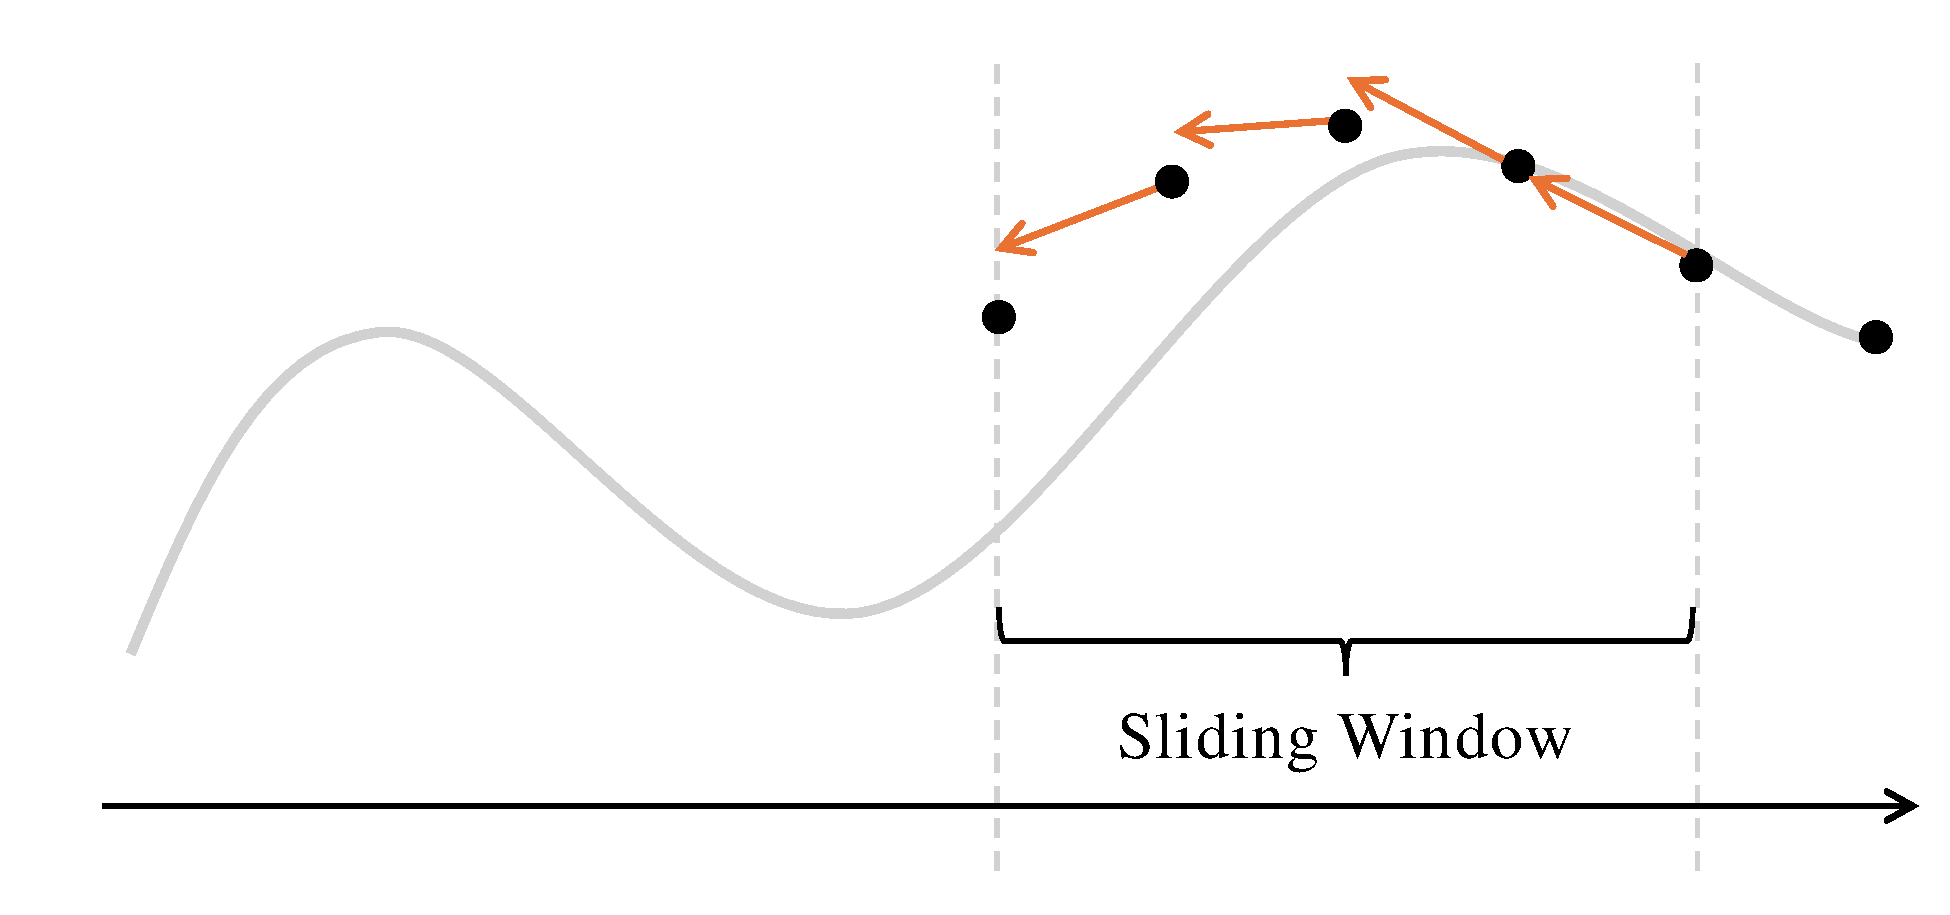
\includegraphics[width=\linewidth]{Images/PartC/paradigm-1.pdf}
        \caption{Compute the drift of $\rvx^{(k)}_{\ell:\ell+p}$ on a batch window of size $p=4$, in parallel}
        \label{fig:picard_1}
    \end{minipage}%
    \hspace{0.03\textwidth} % To maintain the space between the images
    \begin{minipage}[t]{0.30\textwidth}
        \centering
        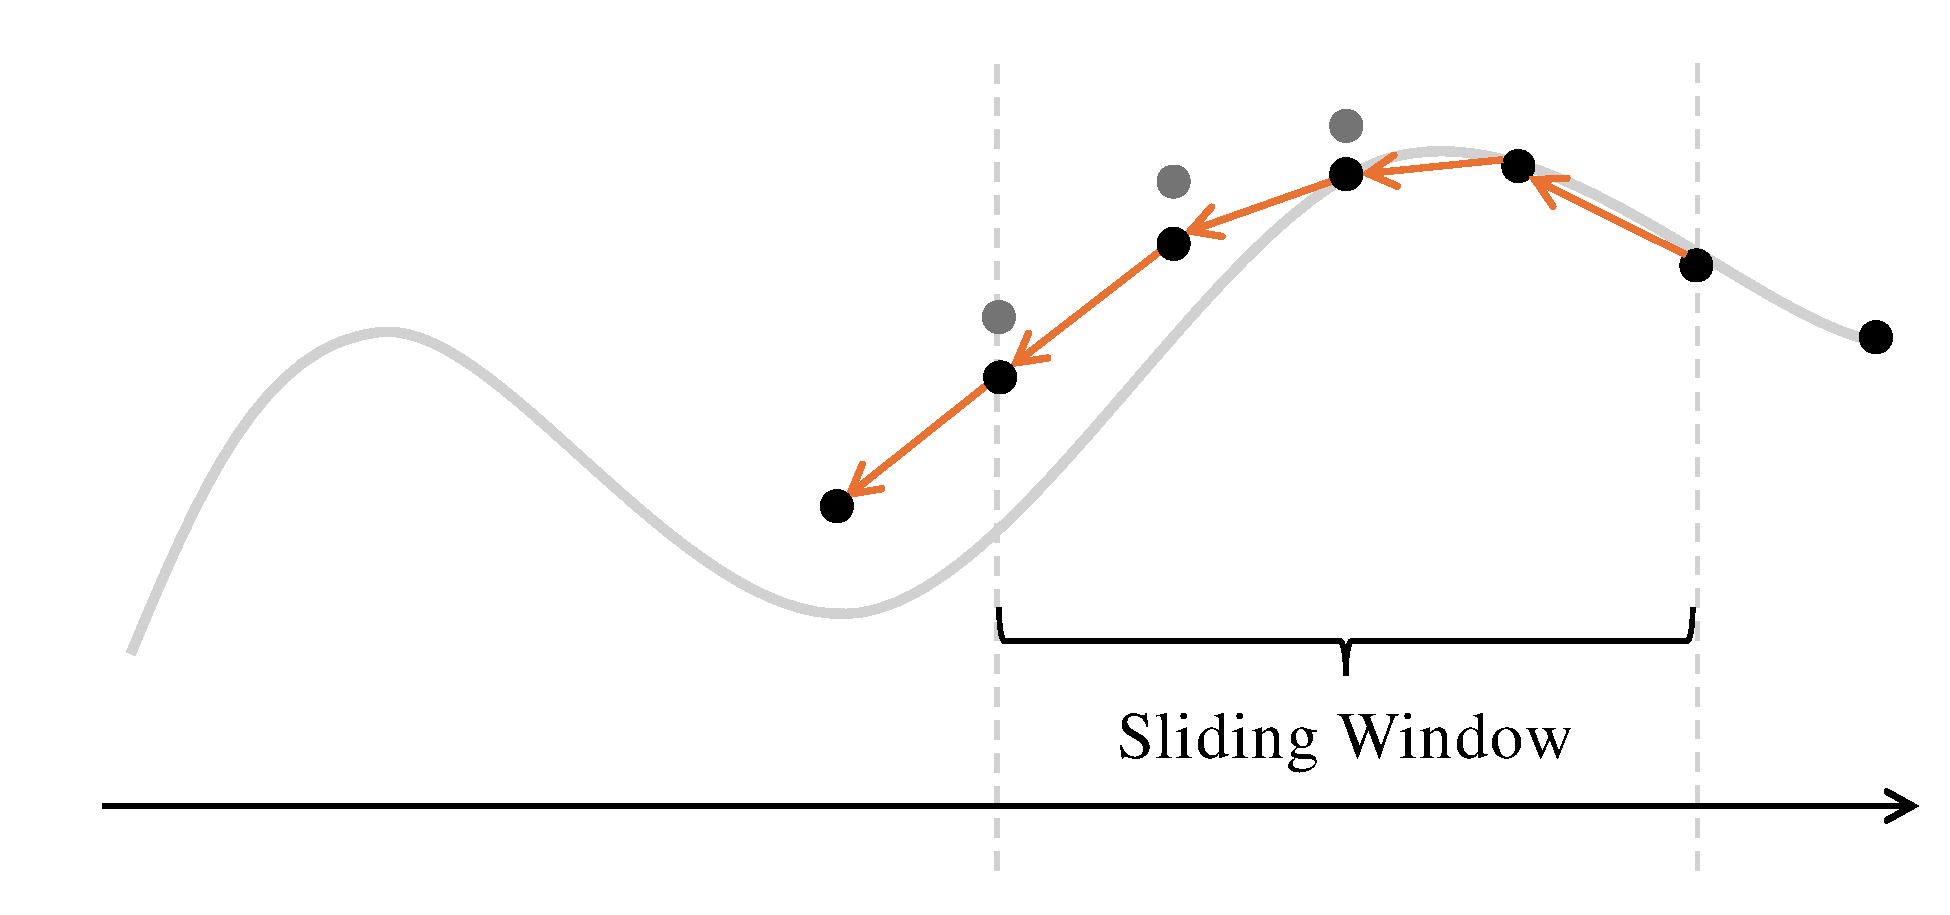
\includegraphics[width=\linewidth]{Images/PartC/paradigm-2.pdf}
        \caption{Update the values to $\rvx^{(k+1)}_{\ell:\ell+p}$ using the cumulative drift of points in the window}
        \label{fig:picard_2}
    \end{minipage}%
    \hspace{0.03\textwidth} % To maintain the space between the images
    \begin{minipage}[t]{0.30\textwidth}
        \centering
        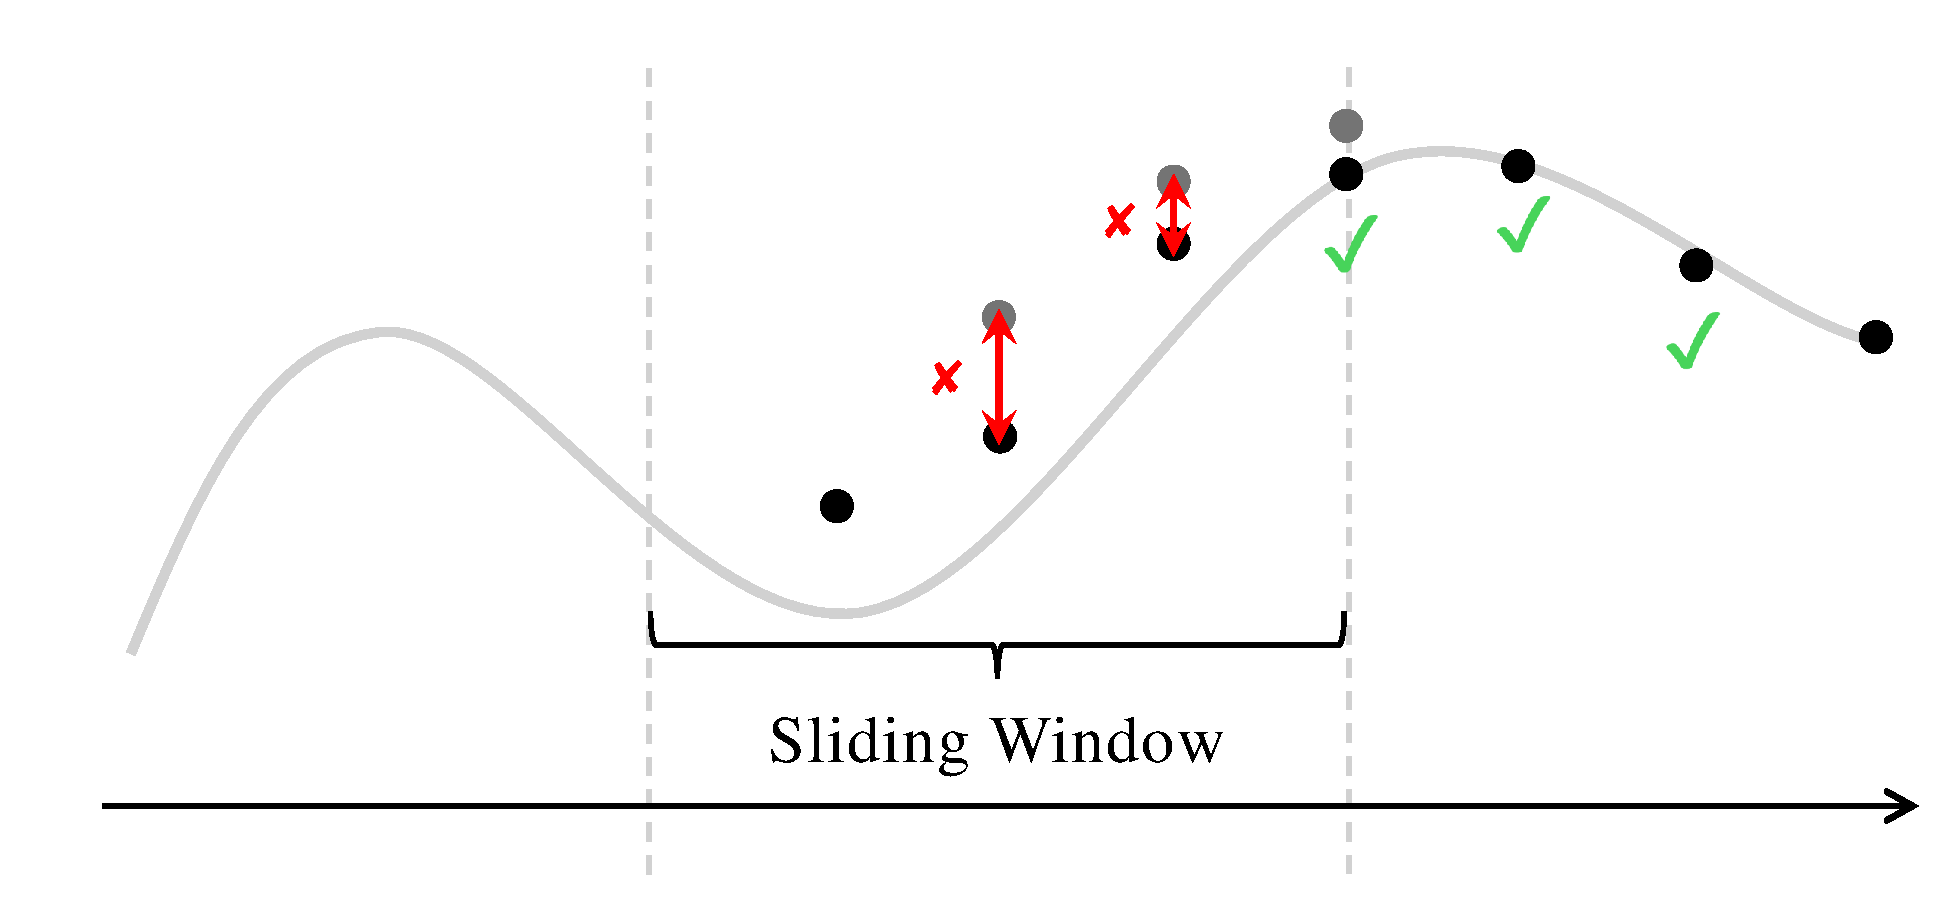
\includegraphics[width=\linewidth]{Images/PartC/paradigm-3.pdf}
        \caption{Determine how far to slide the window forward, based on the error $\lVert \rvx^{(k+1)}_i - \rvx^{(k)}_i \rVert^2$.}
        \label{fig:picard_3}
    \end{minipage}
    % \caption{During iteration $k$, ParaDiGMS processes a batch window of size $p$ spanning timesteps $[t,t+p)$ \textit{in parallel}. The new values at a point $\rvx^{(k+1)}_{t+j}$ are updated based on the value  $\rvx^{(k)}_j$ at the left end of the window, plus the cumulative drift  $1/T \sum_{i=t}^{t+j-1} \mathbf{F}_{\bm{\phi}^\times}(\rvx^{(k)}_{i}, i/T)$  of points within the window. We then slide the window forward until the error exceeds our tolerance, and repeat for the next iteration.}
    \figcredit{Adapted from \citet{shih2023parallel}.}
    \label{fig:picard}
\end{figure}


The discrete Picard update \Cref{eq:discrete_picard_decreasing} expresses
each $\rvx^{(k+1)}_j$ as the fixed initial value $\rvx_T$ minus a cumulative
sum of drifts. To limit memory and exploit parallel hardware, it is convenient
to apply the same idea locally on short, sliding blocks of indices.

Fix a window length $p$ and a left index $\ell$; the window then covers
$j=\ell,\ldots,\ell+p$ with $t_\ell>t_{\ell+1}>\cdots>t_{\ell+p}$. During
iteration $k$:

\subparagraph{Step 1. Parallel Drift Evaluation on the Window.}
Compute, in parallel and using only the previous iterate,
\[
\rvv_{\bphi^\times} \big(\rvx^{(k)}_{\ell+i}, t_{\ell+i}\big),
\quad i=0,1,\ldots,p-1.
\]
These are the $p$ local increments needed to advance from the left edge
$t_\ell$ across the window.

\subparagraph{Step 2. Left–Anchored Cumulative Updates.}
Form the windowed updates by anchoring at $j=\ell$ and accumulating the drift across subintervals:
\begin{equation}\label{eq:window_update}
\rvx^{(k+1)}_{\ell+j+1}
 = 
\rvx^{(k)}_{\ell}
 - \Delta t \sum_{i=0}^{j}
\rvv_{\bphi^\times} \big(\rvx^{(k)}_{\ell+i}, t_{\ell+i}\big),
\quad j=0,1,\ldots,p-1.
\end{equation}
This is the local, windowed counterpart of
\Cref{eq:discrete_picard_decreasing}, with the current left-boundary value
$\rvx^{(k)}_\ell$ serving as the anchor for the window. The minus sign
reflects the decreasing time direction. The inner sum is a prefix sum over
the windowed drifts, so all partial sums can be produced efficiently on
parallel hardware.

\subparagraph{Step 3. Progress Control and Window Advance.}
Having formed the left–anchored cumulative updates on the current window (Step~2),
we now decide how far to slide that window. We measure local convergence
by the pointwise Picard change
\[
\mathtt{error}_j
:=
\big\|\rvx^{(k+1)}_{\ell+j}-\rvx^{(k)}_{\ell+j}\big\|^2,
\quad j=1,\ldots,p-1,
\]
and compare it against prescribed tolerances $\mathtt{tol}_{\ell+j}$. That is, $\mathtt{error}_j$ measures how much the iterate at node $\ell+j$ changed during the last Picard
update. If this number is small, it indicates local agreement between the two
successive approximations and hence local convergence of the fixed-point
iteration at that node. If it is large, that node has not settled yet and needs
more Picard smoothing.


The \emph{stride} is chosen as the first index in the window that fails this
test (or the full window length $p$ if none fail):
\[
\mathtt{stride}
:=
\min\Big(\,\{\,j\ge 1:\ \mathtt{error}_j>\mathtt{tol}_{\ell+j}\,\}\ \cup\ \{p\}\Big).
\]
We then slide the window by setting $\ell \leftarrow \ell+\mathtt{stride}$.  In words: we accept all nodes from the left edge up to (but not including) the
first one that has not converged; if all nodes have converged, we accept the
entire window. We then slide the window by that many accepted nodes,
$\ell \leftarrow \ell+\mathtt{stride}$, and continue. This advances by at
most the window length $p$, never skipping any node that has not met its
tolerance. If sliding would overrun the grid end $M$, we truncate the window to
$p \leftarrow \min\{p,\,M-\ell\}$ and proceed.



When the window moves forward it uncovers new time nodes that
have no values yet. To start Picard iteration there, we simply copy the value
from the left boundary of the window and use it as an initial guess. This
``constant extrapolation'' is cheap and stable, and will be corrected by later
updates. If desired, one can replace it by more accurate guesses, such as linear
or polynomial extrapolations from past points.

This completes the procedure of ParaDiGMS. We summarize the algorithm in \Cref{alg:paradigms}.


\begin{algorithm}[t]
  \caption{ParaDiGMS with Sliding Windows}
  \label{alg:paradigms}
  \begin{algorithmic}[1]
    \Require Drift $\rvv_{\bphi^\times}(\rvx,t)$; $\{t_j\}_{j=0}^{M}$; window length $p$; $\{\mathtt{tol}_j\}_{j=1}^{M}$
    \Ensure Approximate trajectory $\{\rvx^{(k)}_j\}_{j=0}^{M}$ with $\rvx^{(k)}_M$ at $t=0$
    \State $k \gets 0$, $\ell \gets 0$ 
    \State Sample $\rvx^{(0)}_0 \sim p_{\mathrm{prior}}$; set $\rvx^{(0)}_j \gets \rvx^{(0)}_0$ for $j=1,\ldots,\min(p,M)$  \Statex \Comment{constant extrapolation}
    \While{$\ell < M$}
      \State $J \gets \min(p,  M-\ell)$   \Comment{current window length}
      \State \textbfs{Step 1: Parallel} 
      \State For $i=0,\ldots,J-1$: $g_i \gets \rvv_{\bphi^\times} \big(\rvx^{(k)}_{\ell+i},\, t_{\ell+i}\big)$ 
      \Statex \Comment{drifts from previous iterate (Picard freezing)}
      \State Compute prefix sums $S_j \gets \sum_{i=0}^{j} g_i$ for $j=0,\ldots,J-1$ 
      \Statex \Comment{scan over windowed drifts}
      \State \textbfs{Step 2: Cumulative Updates} 
      \State For $j=0,\ldots,J-1$: $\displaystyle \rvx^{(k+1)}_{\ell+j+1} \gets \rvx^{(k)}_{\ell} - \Delta t\, S_j$ 
      \Statex \Comment{left-anchored update; cf.\ \Cref{eq:window_update}}
      \State \textbfs{Step 3: Progress Control and Window Advance} 
      \State For $j=1,\ldots,J-1$: $\mathtt{error}_j \gets \big\|\rvx^{(k+1)}_{\ell+j}-\rvx^{(k)}_{\ell+j}\big\|^2$ \Statex \Comment{pointwise Picard change}
      \State $\displaystyle \mathtt{stride} \gets \min \Big(\,\{\,j\in\{1,\ldots,J-1\}:~\mathtt{error}_j>\mathtt{tol}_{\ell+j}\,\}\ \cup\ \{J\}\Big)$
      \State \textbfs{Initialize New Nodes} 
        \State For $r=1,\ldots,\min\{\mathtt{stride},\,M-\ell-J\}$:
        $\rvx^{(k+1)}_{\ell+J+r}
        \gets
        \rvx^{(k+1)}_{\ell+J}$ 
      \Statex \Comment{constant extrapolation into newly exposed indices}
      \State $\ell \gets \ell + \mathtt{stride}$;\quad $k \gets k+1$
    \EndWhile
    \State \Return $\{\rvx^{(k)}_j\}_{j=0}^{M}$
  \end{algorithmic}
\end{algorithm}




\subsection{Relation to Time-Stepping Solvers}

\paragraph{Selection of Sliding Window Size.}
To understand the role of the window size, first consider the smallest
choice $p=1$. In this case, there is no time parallelism, and the method
reduces to its sequential base update. For the left-endpoint discretization
in \Cref{eq:window_update}, this is simply a plain Euler step.

More generally, ParaDiGMS specifies how computations across different time
points can be parallelized, while the numerical update used at each step can
be chosen separately. For example, the Euler update can be replaced by DDIM
or DPM-Solver, giving ParaDDIM or ParaDPMSolver. Increasing $p$ then exposes
more time points to parallel computation without changing the underlying time
grid or the total number of steps $M$. Picard iteration repeatedly corrects
these states toward consistency with the chosen base solver, with convergence
controlled by the prescribed local tolerances.

\paragraph{Compatibility with Higher--Order Solvers (e.g., DPM).}
The Picard framework determines how states at different time points are updated
and evaluated in parallel, while the numerical rule used to approximate each
step can be chosen separately.

For example, instead of the left-endpoint rule in
\Cref{eq:window_update}, we may use the trapezoidal rule:
\begin{align*}
\rvx^{(k+1)}_{\ell+j+1}
=
\rvx^{(k)}_{\ell}
-\Delta t\Bigg[
\tfrac{1}{2}
\rvv_{\bphi^\times}
\big(\rvx^{(k)}_{\ell},t_{\ell}\big)
+
\sum_{i=1}^{j}
\rvv_{\bphi^\times}
\big(\rvx^{(k)}_{\ell+i},t_{\ell+i}\big)
+
\tfrac{1}{2}
\rvv_{\bphi^\times}
\big(\rvx^{(k)}_{\ell+j+1},t_{\ell+j+1}\big)
\Bigg],
\end{align*}
where $j=0,\ldots,p-1$. For $j=0$, this is the familiar one-step trapezoidal update using the two
endpoint drifts. For larger $j$, the same rule accumulates the trapezoidal
contributions across the window. Since all drifts are evaluated using the
previous Picard iterate, they can still be computed in parallel, while the
interior contributions can be accumulated with a prefix sum.

More generally, ParaDiGMS can use an existing sequential sampler such as
DDIM or DPM-Solver as its base discretization. In that case, the Picard
update is constructed from the corresponding base-solver increment rather
than from the trapezoidal formula above. The precise form depends on the
chosen solver, since higher-order methods may use intermediate stages or
previous model evaluations.

For a ParaDiGMS construction based on a given sequential solver, exact
fixed-point convergence recovers the corresponding sequential discrete
trajectory. With a finite stopping tolerance, the final result also contains
a remaining fixed-point iteration error in addition to the discretization
error of the base solver.

\newpage
\section{Closing Remarks}\label{sec:ch9_cr}

This chapter has confronted one of the most significant practical limitations
of diffusion models: their slow, iterative sampling process. We have explored
training-free approaches that accelerate generation by designing better
numerical solvers for the empirical PF-ODE:
\begin{enumerate}
    \item We began with DDIM, a first-order factored exponential-integrator
    update that retains the known diffusion schedule analytically while
    holding the neural prediction fixed.
    \item We then studied DEIS, which extends this idea to higher-order
    multistep updates by reusing past model evaluations to extrapolate how the
    neural prediction changes.
    \item Finally, we examined the DPM-Solver family, which introduces the
    log-SNR time coordinate and constructs higher-order updates from
    within-step model evaluations. DPM-Solver\texttt{++} further develops
    single-step and multistep variants in the data-prediction formulation.
\end{enumerate}

Together, these methods illustrate a common principle: exploit the analytically
known diffusion structure and concentrate numerical approximation on the
learned model prediction. They differ in the prediction and time
parameterizations, and in whether higher-order information is obtained from
within-step stages or previous-step history. ParaDiGMS provides a complementary
direction by reorganizing computation across time through fixed-point
iteration and parallel evaluation. Such solver developments can reduce the
sampling cost from hundreds or thousands of model evaluations to only tens in
many practical settings.

However, these training-free methods remain fundamentally iterative: they
numerically approximate a continuous generative trajectory, even when parts of
the computation can be parallelized. This raises a natural question:
\emph{can we achieve high-quality generation in just one or a very few steps?}

The final Part~D of this monograph explores this question through
training-based acceleration. In \Cref{ch:distillation}, we study
distillation-based methods, where a fast \textit{student} generator learns to
reproduce the behavior of a slow pre-trained \textit{teacher}. In
\Cref{ch:fast-scratch}, we turn to methods that directly learn few-step
generators from scratch defined by an ODE flow.

This shift from designing a better numerical solver to directly learning a
fast approximation of the generative solution map aims to combine the quality
of diffusion models with the speed of one- or few-step generation.


\clearpage
\newpage
